

%\dominitoc
%\tableofcontents
\chapter{ಭಾಗ : 3 ಬಿಲ್ಲೆಗಳು [Tiles] }\label{chap3}
%\minitoc

\textbf{\Large ವಿಷಯ ಪರಿವಿಡಿ}

\medskip
\medskip

{\renewcommand{\arraystretch}{1.2}
\begin{longtable}[l]{@{}>{}r>{\raggedright}p{9.1cm}>{}r@{}}
\hline
3.1 & ಬಿಲ್ಲೆಗಳ ಪರಿಚಯ \dotfill & \pageref{sec3.1}\\
3.2 & ಗಣಿತದ ಮೂಲ ಪ್ರಕ್ರಿಯೆಗಳನ್ನು ಬಿಲ್ಲೆಗಳ ಸಹಾಯದಿಂದ ತಿಳಿದು ಕೊಳ್ಳುವುದು \dotfill & \raisebox{-0.55cm}{\pageref{sec3.2}}\\
3.3 & ಬಿಲ್ಲೆಗಳ ಸಹಾಯದಿಂದ ಅಪೂರ್ಣಂಕಗಳ ಗುಣಾಕಾರ \dotfill & \pageref{sec3.3}\\
3.4 & ಬಿಲ್ಲೆಗಳ ಅನ್ವಯಗಳು \dotfill  & \pageref{sec3.4}\\
3.5 & ಒಂದು ಏಕ ಪದದಿಂದ ಒಂದು ಬೀಜೋಕ್ತಿಯನ್ನು ಗುಣಿಸುವುದು \dotfill & \pageref{sec3.5}\\
3.6 & ಬಿಲ್ಲೆಗಳ ಸಹಾಯದಿಂದ ಎರಡು ದ್ವಿಪದಗಳ ಗುಣಲಬ್ಧ ಕಂಡು ಹಿಡಿಯುವುದು  \dotfill & \raisebox{-0.55cm}{\pageref{sec3.6}}\\
3.7 & ಬಿಲ್ಲೆಗಳ ಸಹಾಯದಿಂದ ನಿತ್ಯ ಸಮೀಕರಣಗಳನ್ನು ಸಾಧಿಸುವುದು  \dotfill & \pageref{sec3.7}\\
3.8 & ಬಿಲ್ಲೆಗಳ ಸಹಾಯದಿಂದ ಬೀಜೋಕ್ತಿಗಳ ಅಪವರ್ತನಗಳನ್ನು ಕಂಡು ಹಿಡಿಯುವುದು \dotfill & \raisebox{-0.55cm}{\pageref{sec3.8}}\\
3.9 & ಬಿಲ್ಲೆಗಳ ಸಹಾಯದಿಂದ ತ್ರಿಪದಿಗಳನ್ನು ಅಪವರ್ತಿಸುವುದು \dotfill & \pageref{sec3.9}\\
3.10 & ಬಿಲ್ಲೆಗಳ ಸಹಾಯದಿಂದ "ಪೂರ್ಣವರ್ಗ ಮಾಡಿ" ಮಿಶ್ರ ವರ್ಗ ಸಮೀಕರಣಗಳ ಮೂಲಗಳನ್ನು ಕಂಡು ಹಿಡಿಯುವುದು \dotfill & \raisebox{-0.55cm}{\pageref{sec3.10}}\\
3.11 &  ಸಮಾಂತರ ಶ್ರೇಣಿಯ ಮೊದಲ ನಿರ್ಧಿಷ್ಟ ಪದಗಳ $(n)$ ಮೊತ್ತವನ್ನು ಕಂಡು ಹಿಡಿಯುವ ಸೂತ್ರವನ್ನು ಕಂಡುಕೊಳ್ಳುವುದು \dotfill & \raisebox{-0.55cm}{\pageref{sec3.11}}\\
3.12 & ಬಿಲ್ಲೆಗಳ ಸಹಾಯದಿಂದ ಸ್ವಾಭಾವಿಕ ಸಂಖ್ಯೆಗಳ $n$$-$ಪದಗಳ ಮೊತ್ತವನ್ನು ಕಂಡುಹಿಡಿಯುವ ಸೂತ್ರವನ್ನು ಕಂಡುಕೊಳ್ಳುವುದು \dotfill & \raisebox{-0.55cm}{\pageref{sec3.12}}\\[0.5cm]
\hline
\end{longtable}}\relax

\bigskip

\section{ಬಿಲ್ಲೆಗಳ ಪರಿಚಯ}\label{sec3.1}%%% 3.1

ಚೌರಸ ಅಥವಾ ಆಯತ ಆಕಾರದ ಕಾಗದ, ರಟ್ಟು, ಲೋಹದ ಹಾಳೆ ಅಥವಾ ಪ್ಲಾಸ್ಟಿಕ್ ಹಾಳೆಗಳನ್ನು ಗಣಿತದಲ್ಲಿ ಬಿಲ್ಲೆಗಳು [Tiles] ಎಂದು ಕರೆಯುತ್ತಾರೆ. ನಮಗೆ ಅನುಕೂಲಕರ ಅಳೆತೆಗಳಿಂದ ಇವುಗಳನ್ನು ತಯಾರಿಸಲು ಬರುತ್ತದೆ. ಚೌರಸ ಅಥವಾ ಆಯತ ಆಕಾರದಲ್ಲಿ ಬಿಲ್ಲೆಗಳು ಇರುವುದರಿಂದ ಅವುಗಳ ವಿಸ್ತೀರ್ಣ ಅಥವಾ ಕ್ಷೇತ್ರಫಲ ತಿಳಿಯಲು ಸುಲಭ. ಈ ವಿಸ್ತೀರ್ಣದಿಂದ ಬಿಲ್ಲೆಗಳಿಗೆ ಹೆಸರನ್ನು ಕೊಡಲಾಗಿದೆ. ಉದಾಹರಣೆಗಾಗಿ, 
\begin{figure}[H]
\centering
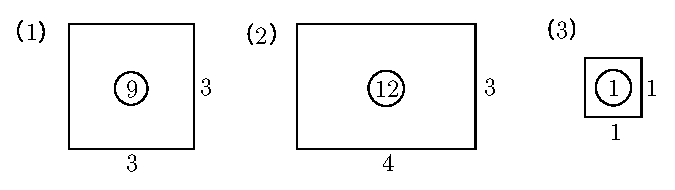
\includegraphics[scale=0.8]{src/figure/chap3/fig3-1.eps}\\
\textbf{\quad 9 ರ ಬಿಲ್ಲೆ  \hspace{1.5cm} \quad 12 ರ ಬಿಲ್ಲೆ \hspace{2cm} 1 ರ ಬಿಲ್ಲೆ }
\end{figure}



ಬಿಲ್ಲೆಗಳಲ್ಲಿ ಎರಡು ಪ್ರಕಾರಗಳು ಇವೆ. 
\begin{itemize}
\item[(1)] ಧನಾತ್ಮಕ ಬಿಲ್ಲೆಗಳು 
\item[(2)] ಋಣಾತ್ಮಕ ಬಿಲ್ಲೆಗಳು 
\end{itemize}
\begin{enumerate}
\item \textbf{ಧನಾತ್ಮಕ ಬಿಲ್ಲೆಗಳು : [Positive Tiles]:} ಬಿಲ್ಲೆಗಳ ವಿಸ್ತೀರ್ಣಗಳು ಧನ ಸಂಖ್ಯೆಯಾಗಿದ್ದರೆ ಅಂತಹ ಬಿಲ್ಲೆಗಳನ್ನು ಧನಾತ್ಮಕ ಬಿಲ್ಲೆಗಳು [Positive Tiles] ಎಂದು ಕರೆಯುತ್ತಾರೆ. ಇಂತಹ ಬಿಲ್ಲೆಗಳನ್ನು ಕಾಗದದ ಮೇಲೆ ತೋರಿಸಲು ವಿಸ್ತೀರ್ಣವನ್ನು ಖಾಲಿ ಜಾಗದಿಂದ ಗುರುತಿಸುತ್ತೆವೆ. 
 
%\eject

\noindent
{\textbf{\underline{ಉದಾಹರಣೆಗಳು: }}}
\begin{figure}[H]
\centering
\includegraphics[scale=0.8]{src/figure/chap3/fig3-2.eps}
\end{figure}

\item \textbf{ಋಣಾತ್ಮಕ ಬಿಲ್ಲೆಗಳು : [Negative Tiles]} ಬಿಲ್ಲೆಗಳ ವಿಸ್ತೀರ್ಣಗಳು ಋಣ ಬೆಲೆಯಾಗಿದ್ದರೆ. ಅಂತಹ ಬಿಲ್ಲೆಗಳನ್ನು ಋಣಾತ್ಮಕ ಬಿಲ್ಲೆಗಳೆಂದು ಕರೆಯುತ್ತಾರೆ. ಇಂತಹ ಬಿಲ್ಲೆಗಳನ್ನು ಕಾಗದದ ಮೇಲೆ ತೋರಿಸಲು ವಿಸ್ತೀರ್ಣವನ್ನು ಗೆರೆಹಾಕಿ ತೋರಿಸುತ್ತಾರೆ.

\noindent
{\textbf{\underline{ಉದಾಹರಣೆಗಳು: }}}
\begin{figure}[H]
\centering
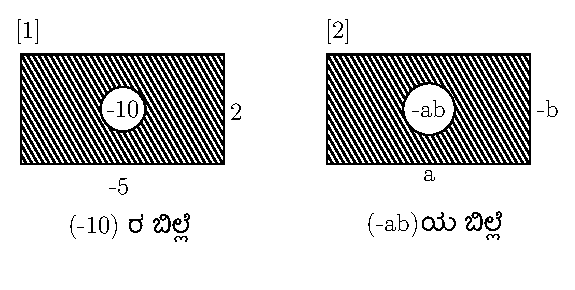
\includegraphics[scale=0.8]{src/figure/chap3/fig3-3.eps}
\end{figure}

ಕೆಲವು ಸಲ ಧನಾತ್ಮಕ ಬಿಲ್ಲೆಗಳನ್ನು ಹಾಗೂ ಋಣಾತ್ಮಕ ಬಿಲ್ಲೆಗಳನ್ನು ಎರಡು ಬೇರೆಬೇರೆ ಬಣ್ಣಗಳಿಂದ ಸೂಚಿಸುತ್ತಾರೆ. ಉದಾಹರಣೆಗಾಗಿ ಧನಾತ್ಮಕ ಬಿಲ್ಲೆಗಳನ್ನು ಕೆಂಪು (Red) ಬಣ್ಣದಿಂದ, ಋಣಾತ್ಮಕ ಬಿಲ್ಲೆಗಳನ್ನು ನೀಲಿ (Blue) ಬಣ್ಣದಿಂದ ಸೂಚಿಸುತ್ತಾರೆ.
%\begin{figure}[H]
%\centering
%\includegraphics[scale=0.8]{src/figure/chap3/fig3-4.eps}
%\end{figure}
\end{enumerate}

\noindent
{\textbf{ಮೂಲಬಿಲ್ಲೆಗಳು :}} ಗಣಿತಗಳಲ್ಲಿ ಬಿಲ್ಲೆಗಳನ್ನು ಉಪಯೋಗಿಸಬೇಕಾದರೆ, ಕೆಲವೊಂದು ಬಿಲ್ಲೆಗಳನ್ನು ನಾವು ಕಡ್ಡಾಯವಾಗಿ ಉಪಯೋಗಿಸಬೇಕಾಗುತ್ತದೆ. ಅವುಗಳಲ್ಲಿ  $+x^2$, $+x$, $+1$ ಹಾಗೂ $-x^{2}$, $-x$, $-1$  ಬಿಲ್ಲೆಗಳು ಮುಖ್ಯವಾಗಿರುತ್ತವೆ. 

%\eject

\begin{enumerate}
\item $[+x^2]$ ಬಿಲ್ಲೆ 
\begin{figure}[H]
\centering
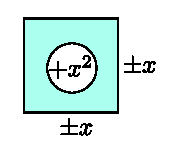
\includegraphics[scale=0.8]{src/figure/chap3/fig3-4a.eps}
\end{figure}

ಇದು ಚೌರಸ ಆಕಾರದ ಬಿಲ್ಲೆ. ಇದರ ಬಾಹುಗಳು ಯಾವುದೇ ಬೆಲೆಯನ್ನು ಹೊಂದಿರಬಹುದು. ಅದಕ್ಕೆ ಇದರ ಬಾಹುಗಳು $(\pm x)$ ಇರುತ್ತವೆ.

\item $(+x)$ ಬಿಲ್ಲೆ 
\begin{figure}[H]
\centering

\includegraphics[scale=0.8]{src/figure/chap3/fig3-4b.eps}
\end{figure}

ಇದು ಆಯತ ಆಕಾರದ ಬಿಲ್ಲೆ. ಇದರ ಬಾಹುಗಳು $(+x)$ ಮತ್ತು $(+1)$ ಅಥವಾ $(-x)$ ಮತ್ತು $(-1)$ ಇರುತ್ತವೆ.

\item $[+1]$ ಬಿಲ್ಲೆ 
\begin{figure}[H]
\centering

\includegraphics[scale=0.8]{src/figure/chap3/fig3-4c.eps}
\end{figure}

ಇದು ಚಿಕ್ಕದಾಗ ಚೌರಸ ಆಕಾರದ ಬಿಲ್ಲೆ. ಇದರ ಬಾಹುಗಳು $(+1)$ ಮತ್ತು $(+1)$ ಅಥವಾ $(-1)$ ಮತ್ತು $(-1)$ ಇರುತ್ತವೆ.

\item $[-x^2]$ ಬಿಲ್ಲೆ  
\begin{figure}[H]
\centering
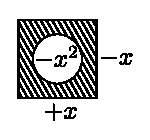
\includegraphics[scale=0.8]{src/figure/chap3/fig3-4d.eps}
\end{figure}

ಇದು ಚೌರಸ ಆಕಾರದ ಬಿಲ್ಲೆಯಾಗಿದೆ. ಇದರ ಬಾಹುಗಳು $(+x)$ ಮತ್ತು $(-x)$ ಅಥವಾ $(-x)$ ಮತ್ತು $(+x)$ ಇರುತ್ತವೆ.

\item $(-x)$ ಬಿಲ್ಲೆ 
\begin{figure}[H]
\centering

\includegraphics[scale=0.8]{src/figure/chap3/fig3-4e.eps}
\end{figure}

ಇದು ಆಯತ ಆಕಾರದ ಬಿಲ್ಲೆಯಾಗಿದೆ. ಇದರ ಉದ್ದ $(+x)$ ಇದ್ದರೆ ಅಗಲವು $(-1)$ ಅಥವಾ ಉದ್ದ $(-x)$ ಇದ್ದರೆ ಅಗಲವು $(+1)$ ಇರುತ್ತವೆ.

\item $(-1)$ ಬಿಲ್ಲೆ 
\begin{figure}[H]
\centering

\includegraphics[scale=0.8]{src/figure/chap3/fig3-4f.eps}
\end{figure}

ಇದೊಂದು ಚೌರಸ ಆಕಾರದ ಬಿಲ್ಲೆಯಾಗಿದೆ. ಇದರ ಬಾಹುಗಳು $(+1)$ ಮತ್ತು $(+1)$ ಅಥವಾ $(-1)$ ಮತ್ತು $(-1)$ ಇರುತ್ತವೆ. 
\end{enumerate}

ಈ ಬಿಲ್ಲೆಗಳನ್ನು ತಯಾರಿಸಬೇಕಾದರೆ, $x^2$ ಬಿಲ್ಲೆಯ ಬಾಹುವಿನಷ್ಟು. $(+x)$ ಬಿಲ್ಲೆಯ ಉದ್ದವಾಗಿರುತ್ತದೆ. ಮತ್ತು ಆಯತದ ಅಗಲವು $(+1)$ ಇದ್ದರೆ.  $(+1)$ ಬಿಲ್ಲೆಯ ಬಾಹುಗಳು $(+1)$ ಇರುತ್ತದೆ.

\noindent
\textbf{ಇತರೇ ಬಿಲ್ಲೆಗಳು :} ಮೂಲಬಿಲ್ಲೆಗಳಲ್ಲದೇ ಸಂದರ್ಭಕ್ಕೆ ತಕ್ಕಂತೆ ಕೆಲವೊಂದು ಬಿಲ್ಲೆಗಳನ್ನು ಉಪಯೋಗಿಸಬೇಕಾಗುತ್ತದೆ. ಅವುಗಳಿಗೆ ಇತರೇ ಬಿಲ್ಲೆಗಳೆಂದು ಕರೆಯುತ್ತಾರೆ.

\noindent
{\textbf{\underline{ಉದಾ :}}} 
\begin{tabular}{llllll}
(1) & $[+ a^2]$ ಬಿಲ್ಲೆ, & (2) & $(+ab)$ ಬಿಲ್ಲೆ & (3) & $(+b^2)$ ಬಿಲ್ಲೆ. 
\end{tabular}

\begin{enumerate}
\item 
~
\begin{figure}[H]
\centering
\includegraphics[scale=0.8]{src/figure/chap3/fig3-5a.eps}
\end{figure}
ಇದು ಚೌರಸ ಆಕಾರದಲ್ಲಿ ಇದ್ದು ಪ್ರತಿಯೊಂದು ಬಾಹು $(\pm a)$ ಅಥವಾ ($\mp$ a) ಇರುತ್ತವೆ. 

\item $[+ab]$ ಬಿಲ್ಲೆ
\begin{figure}[H]
\centering
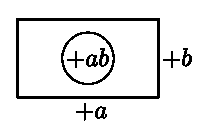
\includegraphics[scale=0.8]{src/figure/chap3/fig3-5b.eps}
\end{figure}
ಇದು ಆಯತ ಆಕಾರದಲ್ಲಿ ಇದ್ದು. ಉದ್ದ $(+a)$ ಮತ್ತು ಅಗಲ $(+b)$ ಅಥವಾ ಉದ್ದ $(-a)$ ಮತ್ತು ಅಗಲ $(-b)$.

\item $[+b^{2}]$	 ಬಿಲ್ಲೆ
\begin{figure}[H]
\centering
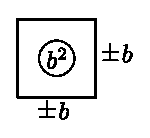
\includegraphics[scale=0.8]{src/figure/chap3/fig3-5c.eps}
\end{figure}
ಇದು ಚೌರಸ ಆಕಾರದಲ್ಲಿದ್ದು ಪ್ರತಿ ಬಾಹು $(+b)$ ಅಥವಾ $(-b)$ ಇರುತ್ತವೆ.

\eject

\item $(-mn)$ ಬಿಲ್ಲೆ 
\begin{figure}[H]
\centering
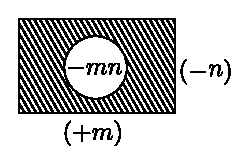
\includegraphics[scale=0.8]{src/figure/chap3/fig3-5d.eps}
\end{figure}
ಇದು ಆಯತ ಆಕಾರದ ಬಿಲ್ಲೆ. ಇದರ ಉದ್ದ $(+m)$ ಇದ್ದರೆ, ಅಗಲ $(-n)$ ಅಥವಾ ವಿರುದ್ಧ. 

\item $[-p^2]$ ಬಿಲ್ಲೆ 
\begin{figure}[H]
\centering

\includegraphics[scale=0.8]{src/figure/chap3/fig3-5e.eps}
\end{figure}
ಇದು ಚೌರಸ ಆಕಾರದ ಬಿಲ್ಲೆ ಇದರ ಒಂದು ಬಾಹು $(+p)$ ಅಥವಾ $(-p)$ ಇರುತ್ತವೆ. ಅಥವಾ ವಿರುದ್ಧ.

\item $[-pq]$ ಬಿಲ್ಲೆ. 
~
\vskip -0.3cm
\begin{figure}[H]
\centering

\includegraphics[scale=0.8]{src/figure/chap3/fig3-5f.eps}
\end{figure}
~
\vskip -0.3cm
ಇದು ಆಯತ ಆಕಾರದ ಬಿಲ್ಲೆ ಇದರ ಉದ್ದ $(+p)$ ಇದ್ದರೆ ಅಗಲ $(-q)$ ಅಥವಾ ವಿರುದ್ಧ. 
\end{enumerate}

\section*{ಗಣಿತ ಕಲಿಕೆ ಮತ್ತು ಬೋಧನೆಯಲ್ಲಿ ಬಿಲ್ಲೆಗಳ ಮಹತ್ವ}

ಬಿಲ್ಲೆಗಳು [Tiles] ಓರಿಗಾಮಿಯಲ್ಲಿ ಒಂದು ಮುಖ್ಯವಾದ ಭಾಗವಾಗಿದ್ದು ಇವುಗಳಿಂದ ಗಣಿತದ ಅನೇಕ ಮುಖ್ಯವಾದ ಪರಿಕಲ್ಪನೆಗಳನ್ನು ಸಾಧಿಸಿ ತೋರಿಸಬಹುದು. ಕಾರಣ ಗಣಿತ ಕಲಿಕೆ ಮತ್ತು ಬೋಧನೆಯಲ್ಲಿ ಬಿಲ್ಲೆಗಳು ಮಹತ್ವದ ಪಾತ್ರವನ್ನು ವಹಿಸುತ್ತವೆ. ಬಿಲ್ಲೆಗಳನ್ನು ಉಪಯೋಗಿಸಿಕೊಂಡು ಕೆಳಗಿನ ಗಣಿತ ಪರಿಕಲ್ಪನೆಗಳನ್ನು ಸಾಧಿಸಲು ಬರುತ್ತದೆ.
\begin{itemize}
\item ಬೀಜಪದಗಳ ಅಥವಾ ಬೀಜೋಕ್ತಿಗಳನ್ನು ಗುಣಾಕಾರ ಮಾಡುವುದು.
\item ಬೀಜೋಕ್ತಿಗಳ ಅಪವರ್ಥನಗಳನ್ನು ಕಂಡು ಹಿಡಿಯುವುದು. 
\item ನಿತ್ಯ ಸಮೀಕರಣಗಳನ್ನು ಪ್ರಾಯೋಗಿಕವಾಗಿ ಸಾಧಿಸುವುದು. 
\item ಮಿಶ್ರ ವರ್ಗ ಸಮೀಕರಣಗಳನ್ನು ಪ್ರಾಯೋಗಿಕವಾಗಿ ಎರಡು ವಿಧಾನಗಳಿಂದ\break ಸಾಧಿಸುವುದು. 
\item ಗಣಿತದ ಮೂಲಕ್ರಿಯೆಗಳಾದ ಸಂಕಲನ, ವ್ಯವಕಲನ, ಗುಣಾಕಾರ ಮತ್ತು ಭಾಗಾ\break ಕಾರಗಳನ್ನು ಪ್ರಾಯೋಗಿಕವಾಗಿ ತಿಳಿದುಕೊಳ್ಳುವುದು. 
\item ಸಮಾಂತರ ಶ್ರೇಣಿಯ ಎಲ್ಲ ಪದಗಳ ಮೊತ್ತ ಕಂಡುಕೊಳ್ಳುವ ಸೂತ್ರಗಳನ್ನು ಪ್ರಾಯೋಗಿಕವಾಗಿ ಸಾಧಿಸುವುದು.
\item ಪೈಥಾಗೋರಾಸದ ಪ್ರಮೇಯನ್ನು ಪ್ರಾಯೋಗಿಕವಾಗಿ ಸಾಧಿಸುವುದು.
\item ಇನ್ನೂ ಕೆಲವು ಗಣಿತ ಪರಿಕಲ್ಪನೆಗಳನ್ನು ಸಾಧಿಸಬಹುದು. 
\end{itemize}

\section{ಗಣಿತದ ಮೂಲ ಪ್ರಕ್ರಿಯೆಗಳನ್ನು ಬಿಲ್ಲೆಗಳ ಸಹಾಯದಿಂದ ತಿಳಿದು\break ಕೊಳ್ಳುವುದು}\label{sec3.2}%3.2

ಪ್ರಾಥಮಿಕ ಮತ್ತು ಪ್ರೌಢಶಾಲಾ ಹಂತದಲ್ಲಿ ಗಣಿತದ ಮುಖ್ಯ ಕಲ್ಪನೆಗಳಾದ ಮೂಲ ಪರಿ\-ಕ್ರಿಯೆ\-ಗಳ ಬೋಧನೆಯಲ್ಲಿ ಲೋಪವಿದೆ ಎಂದು "ವಿಶ್ವವಿದ್ಯಾಲಯ ಧನ ಸಹಾಯ ಆಯೋಗ" [UGC]ದಂತಹ ಸಂಸ್ಥೆಗಳು ತಮ್ಮ ಅಧ್ಯಯನದಲ್ಲಿ ಕಂಡುಕೊಂಡಿವೆ. ಈ ಕಾರಣದಿಂದಲೇ ಗಣಿತ ವಿಷಯವು ಮಕ್ಕಳಲ್ಲಿ ಪ್ರಾರಂಭಿಕ ಹಂತದಲ್ಲಿ "ಕಬ್ಬಿಣದ ಕಡಲೆ"ಯಾಗಿದೆ. ಚಟುವಟಿಕೆಗಳ ಮೂಲಕ ಬಿಲ್ಲೆಗಳ ಸಹಾಯದಿಂದ ಮೂಲ ಕ್ರಿಯೆಗಳನ್ನು ಸರಿಯಾಗಿ ತಿಳಿದುಕೊಂಡರೆ, "ಕಬ್ಬಿಣದ ಕಡಲೆ"ಯನ್ನು ಸಹ ಕರಗಿಸಿಕೊಳ್ಳುವ ಸಾಮರ್ಥ್ಯ ಮಕ್ಕಳಲ್ಲಿ ತಾನಾಗಿಯೇ ಬರುತ್ತದೆ ಎಂಬ ಸಂಗತಿ ಕಲಿಕೆ ಮತ್ತು ಬೋಧನೆಯಲ್ಲಿ "ಓರಿಗಾಮಿ" ಉಪಯೋಗಿಸುವುದರಿಂದ ತಿಳಿದು ಬಂದಿದೆ. ಬಿಲ್ಲೆಗಳ ಸಹಾಯದಿಂದ ಮೂಲಕ್ರಿಯೆಗಳನ್ನೂ ತಿಳಿದುಕೊಳ್ಳಬೇಕಾದರೆ, ಮೊದಲು "ತಟಸ್ಥೀಕರಣ ನಿಯಮ"ವನ್ನು ತಿಳಿದು ಕೊಳ್ಳಬೇಕು.

\medskip
\noindent
\textbf{\underline{ತಟಸ್ಥೀಕರಣ ನಿಯಮ :}} ಯಾವುದೇ ವ್ಯವಸ್ಥೆಗೆ [ಬೆಲೆಗೆ] ಧನ ಬೆಲೆಯಷ್ಟೇ ಋಣಬೆಲೆ\-ಯನ್ನು ಸೇರಿಸಿದರೆ ಅಥವಾ ಕಡಿಮೆ ಮಾಡಿದರೆ, ಆವ್ಯವಸ್ಥೆಯ ಬೆಲೆ ವ್ಯತ್ಯಾಸವಾಗುವುದಿಲ್ಲ. \hbox{ಅಂದರೆ}, ಒಂದು ಧನ ಬೆಲೆಗೆ ಅಷ್ಟೆ ಋಣ ಬೆಲೆಯನ್ನು ಸೇರಿಸುವುದರಿಂದ ಒಟ್ಟು ಬೆಲೆ ಸೊನ್ನೆ [0]ಯಾಗುತ್ತದೆ. ಕೆಳಗಿನ ಉದಾಹರಣೆಗಳಲ್ಲಿ ಬಿಲ್ಲೆಗಳ ಸಹಾಯದಿಂದ ಪರೀಕ್ಷಿಸೋಣ.

\noindent
\textbf{\underline{ಉದಾ :}}
\begin{itemize}
\item[(1)]
~
\begin{figure}[H]
\centering
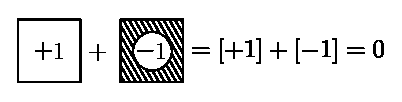
\includegraphics[scale=0.8]{src/figure/chap3/fig3-6a.eps}
\end{figure}
 
\item[(2)] 
~
\begin{figure}[H]
\centering
\includegraphics[scale=0.8]{src/figure/chap3/fig3-6b.eps}
\end{figure} 

\item[(3)] 
~
\begin{figure}[H]
\centering
\includegraphics[scale=0.8]{src/figure/chap3/fig3-6c.eps}
\end{figure}
 \end{itemize}

ಬಿಲ್ಲೆಗಳ ಸಹಾಯದಿಂದ "ತಟಸ್ಥೀಕರಣ ನಿಯಮ"ವನ್ನು ಸಾಧಿಸುವಾಗ ಕೆಳಗಿನ ಸಂಗತಿಗಳನ್ನು ತಿಳಿದುಕೊಂಡಿರಬೇಕು.
\begin{itemize}
\item ಹಾಕುವದು ಅಥವಾ ಸೇರಿಸುವದು ಎಂದರೆ, ಗಳಿಸುವಿಕೆ ಅಥವಾ ಲಾಭವಾಗುವಿಕೆ. ಇವುಗಳನ್ನು ಸಂಕಲನ $[+]$ ಎಂದು ತಿಳಿಯಬೇಕು. 

\item ತೆಗೆಯುವದು ಅಥವಾ ಕಡಿಮೆ ಮಾಡುವದು ಎಂದರೆ ಖರ್ಚು ಮಾಡುವದು ಅಥವಾ ಕೊಡುವದು ಇವುಗಳನ್ನು ವ್ಯವಕಲನ $[-]$ ಎಂದು ತಿಳಿಯಬೇಕು. ಕೆಳಗಿನ ಉದಾಹರಣೆಗಳಿಂದ ಇದನ್ನು ತಿಳಿದುಕೊಳ್ಳಬಹುದು.

\noindent
\textbf{\underline{ಉದಾ : [1]}} $[+3]$ಕ್ಕೆ $[+1]$ ಮತ್ತು $[-1]$ ಇವುಗಳ ಒಂದು ಜೊತೆ ಬಿಲ್ಲೆಗಳನ್ನು ಸೇರಿಸುವುದರಿಂದ ಮೊದಲಿನ ಬೆಲೆ ವ್ಯತ್ಯಸವಾಗುವುದಿಲ್ಲ. ಬಿಲ್ಲೆಗಳ ಸಹಾಯದಿಂದ ಸಾಧಿಸುವದು. 
%\begin{figure}[H]
%\centering
%\includegraphics[scale=0.8]{src/figure/chap3/fig3-7a.eps}
%\end{figure}
\begin{figure}[H]
\centering
\includegraphics[scale=0.8]{src/figure/chap3/fig3-7b.eps}
\end{figure}

\begin{itemize}
\item[*] ಚಿತ್ರದಲ್ಲಿ ತೋರಿಸಿದಂತೆ, $[+3]$ದ ಬಿಲ್ಲೆಗಳ ಜೊತೆಗೆ $[+]$ ಮತ್ತು $[-1]$ರ ಒಂದು ಜೊತೆ ಬಿಲ್ಲೆಗಳನ್ನು ಸೇರಿಸಿದಾಗ, ಒಟ್ಟು $[+4]$ ಬಿಲ್ಲಿಗಳು ಮತ್ತು $[-1]$ ಬಿಲ್ಲೆಯುಂಟಾಗುತ್ತವೆ. ಅವುಗಳಲ್ಲಿ $[+1]$ರ ಬಿಲ್ಲೆ ಮತ್ತು $[-1]$ರ ಬಿಲ್ಲೆಯ ಜೋಡಿಗಳನ್ನು ತೆಗೆದಾಗ ಕೇವಲ. $[+ 1]$ರ 3 ಬಿಲ್ಲೆಗಳು ಉಳಿಯುತ್ತವೆ.

\item[*] ಚಿತ್ರದಲ್ಲಿ ತೋರಿಸಿದಂತೆ ರೇಖಾ ಚಿತ್ರದಿಂದ ತೋರಿಸಬಹುದು.
\end{itemize}
\end{itemize}

\noindent
\medskip
\textbf{ಸಂಕಲನ :} $[+1]$ರ  ಬಿಲ್ಲೆ, ಮತ್ತು $[-1]$ರ  ಬಿಲ್ಲೆಗಳನ್ನು ಉಪಯೋಗಿಸಿ ಸಂಕಲನ ಕ್ರಿಯೆ\break ಯನ್ನು ತಿಳಿದುಕೊಳ್ಳುವುದು.

\noindent
{\textbf{\underline{ಉದಾ: 1 :}}} $[+2] + [+3] = ?$

\noindent
{\textbf{\underline{ಹಂತಗಳು:}}} (1) ಎರಡು $[+1]$ರ ಬಿಲ್ಲೆಗಳನ್ನು $[+1]$ರ 3 ಬಿಲ್ಲೆಗಳನ್ನು ರೇಖಾಚಿತ್ರದಲ್ಲಿ\break ತೋರಿಸಿದಂತೆ ಜೋಡಿಸಬೇಕು.
%\begin{figure}[H]
%\centering
%\includegraphics[scale=0.8]{src/figure/chap3/fig3-8a.eps}
%(ಚಿತ್ರ - 1)
%\end{figure}

%(2) ರೇಖಾಚಿತ್ರ ಉಪಯೋಗಿಸಿ ತೋರಿಸಲು ಬರುತ್ತದೆ. (ಚಿತ್ರ -2)
\begin{figure}[H]
\centering
\includegraphics[scale=0.8]{src/figure/chap3/fig3-8b.eps}
\end{figure}

%\eject

\noindent
{\textbf{\underline{ಉದಾ: 2:}}} $[+3] + [-2] = ?$

\noindent
{\textbf{\underline{ಹಂತಗಳು}}} 
\begin{itemize}
\item[(1)] ಚಿತ್ರ -1 ರಲ್ಲಿ ತೋರಿಸಿದಂತೆ $[+1]$ರ 3 ಬಿಲ್ಲೆಗಳಿಗೆ $[-1]$ರ ಎರಡು ಬಿಲ್ಲೆಗಳನ್ನು\break ಸೇರಿಸಿದಾಗ ಉಂಟಾಗುವ ಬಿಲ್ಲೆಗಳಲ್ಲಿ $(+2) + (-2) = 0$ ಬೆಲೆಯ ಬಿಲ್ಲೆಗಳನ್ನು ಹೊರ ತೆಗೆದಾಗ, ಕೇವಲ $[+1]$ರ ಒಂದು ಬಿಲ್ಲೆ ಉಳಿಯುತ್ತದೆ.
%\begin{figure}[H]
%\centering
%\includegraphics[scale=0.8]{src/figure/chap3/fig3-9a.eps}
%(ಚಿತ್ರ - 1)
%\end{figure}
%ಬಿಲ್ಲೆಗಳನ್ನು ಸೇರಿಸಿದಾಗ, 

$\therefore [+3] + [-2] = [+1]$ ರೇಖಾಚಿತ್ರದಲ್ಲಿ ತೋರಿಸಲು ಬರುತ್ತದೆ.
\begin{figure}[H]
\centering
\includegraphics[scale=0.8]{src/figure/chap3/fig3-9b.eps}
\end{figure}
%ಚಿತ್ರ -2ರಲ್ಲಿ ತೋರಿಸಿದಂತೆ ರೇಖಾಚಿತ್ರದಿಂದ ತೋರಿಸಲು ಬರುತ್ತದೆ. 

$\therefore [+3] + [-2] = [+1]$
\end{itemize}

\medskip
\noindent
{\textbf{\underline{ಉದಾ: 3 :}}} $[-3] + [+2] = ?$

\noindent
{\textbf{\underline{ಹಂತಗಳು : (1)}}}  $[-1]$ದ 3 ಬಿಲ್ಲೆಗಳನ್ನು ಮತ್ತು $[+1]$ರ 2 ಬಿಲ್ಲೆಗಳನ್ನು ಜೋಡಿಸಿದಾಗ ಚಿತ್ರ -1 ರಲ್ಲಿ ತೋರಿಸಿದಂತೆ ಬಿಲ್ಲೆಗಳು ಇರುತ್ತವೆ. ಈಗ $(+1)$ರ 2 ಬಿಲ್ಲೆಗಳನ್ನು ಮತ್ತು $[-1]$ರ 2 ಬಿಲ್ಲೆಗಳನ್ನು ಹೊರ ತೆಗೆದಾಗ $[+1]$ರ 1 ಬಿಲ್ಲೆ ಉಳಿಯುತ್ತದೆ.
%\begin{figure}[H]
%\centering
%\includegraphics[scale=0.8]{src/figure/chap3/fig3-10a.eps}
%(ಚಿತ್ರ - 1)
%\end{figure}

ಇದನ್ನು ರೇಖಾಚಿತ್ರದಿಂದ ತೋರಿಸಲು ಬರುತ್ತದೆ.
\begin{figure}[H]
\centering
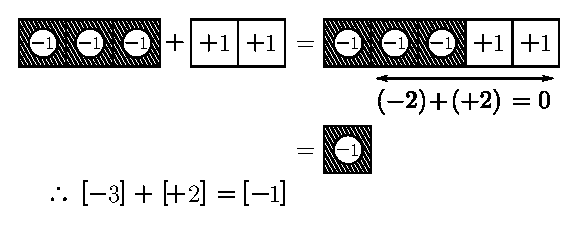
\includegraphics[scale=0.8]{src/figure/chap3/fig3-10b.eps}
\end{figure}
$\therefore \ [-3]+[+2]=[-1]$

\noindent
{\textbf{\underline{ಉದಾ: 4:}}} $[-3] + [-2] = ?$

\noindent
{\textbf{\underline{ಹಂತ : 1 :}}} $[-1]$ರ 3 ಬಿಲ್ಲೆಗಳನ್ನು ಮತ್ತು $[-1]$ರ 2 ಬಿಲ್ಲೆಗಳನ್ನು ಚಿತ್ರದಲ್ಲಿ ತೋರಿಸಿದಂತೆ ಜೋಡಿಸಬೇಕು. ಆಗ $[-1]$ರ 5 ಬಿಲ್ಲೆಗಳು ಆಗುತ್ತವೆ.
%\begin{figure}[H]
%\centering
%\includegraphics{src/figure/chap3/fig3-11a.eps}
%(ಚಿತ್ರ - 1)
%\end{figure}

%\eject

ಇದನ್ನು ರೇಖಾಚಿತ್ರದಲ್ಲಿ ತೋರಿಸಬಹುದು.
\begin{figure}[H]
\centering
\includegraphics{src/figure/chap3/fig3-11b.eps}
(ಚಿತ್ರ - 2)
\end{figure}

$\therefore [-3] + [-2] = [-5]$

%ಚಿತ್ರ -2 ರಲ್ಲಿ ತೋರಿಸಿದಂತೆ. ಇದನ್ನು ರೇಖಾಚಿತ್ರದಿಂದ ತೋರಿಸಲು ಬರುತ್ತದೆ. 

\noindent
\medskip
{\textbf{\underline{ವ್ಯವಕಲನ :}}} ಮೂಲಕ್ರಿಯೆಗಳಲ್ಲಿ ವ್ಯವಕಲನವೆಂದರೆ, ತೆಗೆಯುವದು ಅಥವಾ ಕಡಿಮೆ ಮಾಡು\-ವದು ಎಂದು ಅರ್ಥವಾಗುತ್ತದೆ. ಈ ಕ್ರಿಯೆಯನ್ನು ಬಿಲ್ಲೆಗಳ ಸಹಾಯದಿಂದ ಕಂಡುಕೊಳ್ಳ\break ಬಹುದು.

\noindent
{\textbf{\underline{ಉದಾ: 1 :}}} $[+4] - [+2] = ?$

ಚಿತ್ರದಲ್ಲಿ ತೋರಿಸಿದಂತೆ $[+1]$ರ 4 ಬಿಲ್ಲೆಗಳನ್ನು ತೆಗೆದುಕೊಂಡು ಅವುಗಳಲ್ಲಿ $[+1]$ರ 2 ಬಿಲ್ಲೆಗಳನ್ನು ತೆಗೆದಾಗ ಅಥವಾ ಕಡಿಮೆ ಮಾಡಿದಾಗ $[+1]$ರ 2 ಬಿಲ್ಲೆಗಳು ಉಳಿಯುತ್ತವೆ. ಇದನ್ನು  ರೇಖಾ ಚಿತ್ರದ ಮೂಲಕ ತೋರಿಸಬಹುದು.
%~ \begin{figure}[H]
%~ \centering
%~ \includegraphics{src/figure/chap3/fig3-12a.eps}
%~ (ಚಿತ್ರ - 1)
%~ \end{figure}
\begin{figure}[H]
\centering
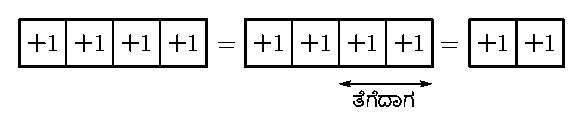
\includegraphics{src/figure/chap3/fig3-12b.eps}
%(ಚಿತ್ರ - 2)
\end{figure}

$\therefore [+4] - [+2] = [+2]$

\noindent
{\textbf{\underline{ಉದಾ: 2 :}}} $[+2] - [+4] = ?$

ಈ ಉದಾಹರಣೆಯಲ್ಲಿ $[+1]$ರ 2 ಬಿಲ್ಲೆಗಳಲ್ಲಿ $[+1]$ರ 4 ಬಿಲ್ಲೆಗಳನ್ನು ಕಡಿಮೆ ಮಾಡಲು ಬರುವದಿಲ್ಲ. ಕಾರಣ $[+1]$ರ ಎರಡು ಬಿಲ್ಲೆಗಳ ಜೊಡಿಸಿ $[+1]$ರ ಎರಡು ಬಿಲ್ಲೆಗಳನ್ನು ಮತ್ತು $[-1]$ರ ಎರಡು ಬಿಲ್ಲೆಗಳನ್ನು ಸೇರಿಸಬೇಕು. ಈಗ $[+1]$ರ 4 ಬಿಲ್ಲೆಗಳು ಮತ್ತು $[-1]$ರ ಎರಡು ಬಿಲ್ಲೆಗಳು ಉಂಟಾಗುತ್ತವೆ. ಈಗ ನಾವು ಈ ವ್ಯವಸ್ಥೆಯಲ್ಲಿ $[+1]$ರ 4 ಬಿಲ್ಲೆಗಳನ್ನು ಕಡಿಮೆ ಮಾಡಬಹುದು. ಬಿಲ್ಲೆಗಳನ್ನು ಚಿತ್ರದಲ್ಲಿ  ತೋರಿಸಿದಂತೆ ಜೋಡಿಸಬೇಕು. 
%~ \begin{figure}[H]
%~ \centering
%~ \includegraphics[scale=0.9]{src/figure/chap3/fig3-13a.eps}
%~ (ಚಿತ್ರ - 1)
%~ \end{figure}

ಈಗ ಉಂಟಾದ ವ್ಯವಸ್ಥೆಯಲ್ಲಿ $[+1]$ರ 4 ಬಿಲ್ಲೆಗಳನ್ನು ತೆಗೆದಾಗ ಕೇವಲ $[-1]$ರ ಎರಡು ಬಿಲ್ಲೆಗಳು ಉಳಿಯುತ್ತವೆ.

$\therefore [+2] - [+4] = [-2]$

%\eject

ಇದನ್ನು  ರೇಖಾಚಿತ್ರದಲ್ಲಿ ತೋರಿಸಲಾಗಿದೆ. 
\begin{figure}[H]
\centering
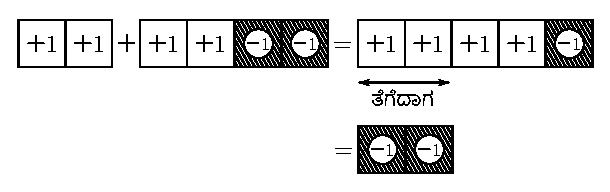
\includegraphics[scale=0.8]{src/figure/chap3/fig3-13b.eps}
\end{figure}

\noindent
{\textbf{\underline{ಉದಾ: 3 :}}} $[+4] - [-2] = ?$

ಈ ಉದಾಹರಣೆಯಲ್ಲಿ $[+1]$ರ 4 ಬಿಲ್ಲೆಗಳಲ್ಲಿ $[-1]$ರ ಎರಡು ಬಿಲ್ಲೆಗಳನ್ನು ಕಡೆಮೆ ಮಾಡಲು [ತೆಗೆಯಲು] ಸಾಧ್ಯವಿಲ್ಲ. ಕಾರಣ ತಟಸ್ಥೀಕರಣ ನಿಯಮದ ಪ್ರಕಾರ ಈ ವ್ಯವಸ್ಥೆಗೆ $[+1]$ರ 2 ಬಿಲ್ಲೆಗಳನ್ನು ಮತ್ತು $[-1]$ರ 2 ಬಿಲ್ಲೆಗಳನ್ನು ಸೇರಿಸಬೇಕು. ಈಗ ಚಿತ್ರದಲ್ಲಿ ತೋರಿಸಿದಂತೆ $[-1]$ರ 2 ಬಿಲ್ಲೆಗಳನ್ನು ಕಡಿಮೆ ಮಾಡಿದರೆ ಉಳಿದ ಬಿಲ್ಲೆಗಳು ಉದಾಹರಣೆಯ ಬೆಲೆಯಾಗುತ್ತದೆ. 
%~ \begin{figure}[H]
%~ \centering
%~ \includegraphics[scale=0.8]{src/figure/chap3/fig3-14a.eps}
%~ (ಚಿತ್ರ - 1)
%~ \end{figure}
%~ 
%~ ಚಿತ್ರದಲ್ಲಿ ತೋರಿಸಿದಂತೆ 
%~ \begin{align*}
%~ [+4] + [(+2) + (-2)] = [(+6) + (-2)] & = [+6]\\
%~ \therefore [+4] - [2] & = [+6]
%~ \end{align*}

ಇದನ್ನು ಚಿತ್ರದಲ್ಲಿ ತೋರಿಸಿದಂತೆ ಬಿಲ್ಲೆಗಳ ಸಹಾಯದಿಂದ ರೇಖಾಚಿತ್ರದಿಂದ ತೋರಿಸಬಹುದು. 
\begin{figure}[H]
\centering
\includegraphics[scale=0.8]{src/figure/chap3/fig3-14b.eps}
\end{figure}
\begin{align*}
[+4]+[(+2)+(-2)] &= [(+6)+(-2)]\quad \text{2 ಬಿಲ್ಲೆಗಳನ್ನು ತೆಗೆದಾಗ}\\
                 &= [+6]\\
                 \therefore ~~ [+4] - [-2] & = [+6]
\end{align*}
\noindent
{\textbf{\underline{ಉದಾ: 4 :}}} $[-4] - [+2] = ?$

ಈ ಉದಾಹರಣೆಯಲ್ಲಿ $[-1]$ರ 4 ಬಿಲ್ಲೆಗಳಲ್ಲಿ $[+1]$ರ 2 ಬಿಲ್ಲೆಗಳನ್ನು ಕಡಿಮೆ ಮಾಡಲು ಅಥವಾ ತೆಗೆದುಹಾಕಲು ಸಾಧ್ಯವಿಲ್ಲ. ಕಾರಣ ತಟಸ್ಥೀಕರಣ ನಿಯಮದ ಸಹಾಯದಿಂದ $[+1]$ರ 2 ಬಿಲ್ಲೆಗಳನ್ನು ಮತ್ತು $[-1]$ರ 2 ಬಿಲ್ಲೆಗಳನ್ನು ಸೇರಿಸಬೇಕು. ಆಗ $[+1]$ರ 2\break ಬಿಲ್ಲೆಗಳು ಮತ್ತು $[-1]$ರ 6 ಬಿಲ್ಲೆಗಳು ಆಗುತ್ತವೆ. ಈಗ $[+1]$ರ 2 ಬಿಲ್ಲೆಗಳನ್ನು ತೆಗೆದುಕೊಳ್ಳಲು ಬರುತ್ತದೆ. ಉಳಿಯುವ $[-1]$ರ 6 ಬಿಲ್ಲೆಗಳು ಈ ಉದಾಹರಣೆಯ ಉತ್ತರವಾಗಿರುತ್ತದೆ. ಚಿತ್ರದಲ್ಲಿ ತೋರಿಸಿದಂತೆ ರೇಖಾಚಿತ್ರದಿಂದ ತೋರಿಸಬಹುದು.
%~ \begin{figure}[H]
%~ \centering
%~ \includegraphics[scale=0.8]{src/figure/chap3/fig3-15a.eps}
%~ (ಚಿತ್ರ - 1)
%~ \end{figure}
%~ 
%~ ಚಿತ್ರ - 1 ರ ಸಹಾಯದಿಂದ 
%~ \begin{align*}
%~ [-4] + [(+2) + (-2)] & = [-6] + [+2] = [-6]\\
%~ \therefore [-4] - [+2] & = [-6]
%~ \end{align*}
%~ 
%~ ಇದನ್ನು ರೇಖಾ ಚಿತ್ರದಿಂದ ಚಿತ್ರ - 2 ರಲ್ಲಿ ತೋರಿಸಿದಂತೆ ತೋರಿಸಬಹುದು. 

ಇದನ್ನು ಚಿತ್ರದಲ್ಲಿ ತೋರಿಸಿದಂತೆ ಬಿಲ್ಲೆಗಳ ಸಹಾಯದಿಂದ ರೇಖಾಚಿತ್ರದಿಂದ ತೋರಿಸಬಹುದು.
\begin{figure}[H]
\centering
\includegraphics[scale=0.8]{src/figure/chap3/fig3-15b.eps}
%(ಚಿತ್ರ - 2)
\end{figure}
$\therefore \ [-4]+[(+2)+(-2)]=[-6]+[+2]=[-6]$\qquad $[+2]$ ತೆಗೆಯಲಾಗಿದೆ.


\noindent
{\textbf{\underline{ಉದಾ: 5 :}}} $[-4] - [-2] = ?$

ಈ ಉದಾಹರಣೆಯಲ್ಲಿ $[-1]$ರ 4 ಬಿಲ್ಲೆಗಳಲ್ಲಿ $[-1]$ರ 2 ಬಿಲ್ಲೆಗಳನ್ನು ಸುಲಭವಾಗಿ ತೆಗೆಯ\-ಬಹುದು. ಉಳಿದ $[-1]$ರ 2 ಬಿಲ್ಲೆಗಳು ಈ ಉದಾಹರಣೆಯ ಉತ್ತರವಾಗಿರುತ್ತದೆ. ಚಿತ್ರದಲ್ಲಿ ತೋರಿಸಿದಂತೆ ಬಿಲ್ಲೆಗಳನ್ನು ಜೋಡಿಸಬಹುದು ಹಾಗೂ ರೇಖಾಚಿತ್ರದಿಂದ ಸೂಚಿಸಬಹುದು. 
%~ \begin{figure}[H]
%~ \centering
%~ \includegraphics[scale=0.8]{src/figure/chap3/fig3-16a.eps}
%~ (ಚಿತ್ರ - 1)
%~ \end{figure}
\begin{figure}[H]
\centering
\includegraphics[scale=0.8]{src/figure/chap3/fig3-16b.eps}
%(ಚಿತ್ರ - 2)
\end{figure}

ಚಿತ್ರದ ಸಹಾಯದಿಂದ, 
~
\vskip -0.5cm
$$
[-4] - [-2] = [-2]
$$


\noindent
{\textbf{\underline{ಉದಾ: 6:}}} $[-2] - [-4] = ?$

ಈ ಉದಾಹರಣೆಯಲ್ಲಿ $[-1]$ರ 2 ಬಿಲ್ಲೆಗಳಲ್ಲಿ $[-1]$ರ 4 ಬಿಲ್ಲೆಗಳನ್ನು ಕಡಿಮೆ\break ಮಾಡಲು ಅಥವಾ ಹೊರ ತೆಗೆಯುವುದು ಸಾಧ್ಯವಿಲ್ಲ. ಕಾರಣ ತಟಸ್ಥೀಕರಣ ನಿಯಮದ\break  ಪ್ರಕಾರ $[-1]$ರ 2 ಬಿಲ್ಲೆಗಳಲ್ಲಿ $[+1]$ರ 2 ಬಿಲ್ಲೆಗಳನ್ನು ಮತ್ತು $[-1]$ರ 2 ಬಿಲ್ಲೆಗಳನ್ನು ಸೇರಿಸ\break ಬೇಕು. ಆಗ $[+1]$ರ 2 ಬಿಲ್ಲೆಗಳು ಮತ್ತು $[-1]$ರ 4 ಬಿಲ್ಲೆಗಳು ಉಂಟಾಗುತ್ತವೆ. ಈ $[-1]$ರ 4 ಬಿಲ್ಲೆಗಳನ್ನು ತೆಗೆದಾಗ ಉಳಿಯುವ $[+1]$ರ ಎರಡು ಬಿಲ್ಲೆಗಳು ಉತ್ತರವಾಗಿದೆ. ಬಿಲ್ಲೆಗಳನ್ನು ಚಿತ್ರದಲ್ಲಿ ತೋರಿಸಿದಂತೆ ಜೋಡಿಸಬೇಕು. ಹಾಗೆ ರೇಖಾಚಿತ್ರದಿಂದ ತೋರಿಸಬಹುದು. 
%~ \begin{figure}[H]
%~ \centering
%~ \includegraphics[scale=0.8]{src/figure/chap3/fig3-17a.eps}
%~ (ಚಿತ್ರ - 1)
%~ \end{figure}
\begin{figure}[H]
\centering
\includegraphics[scale=0.8]{src/figure/chap3/fig3-17b.eps}
%~ (ಚಿತ್ರ - 2)
\end{figure}

ಚಿತ್ರಗಳ ಸಹಾಯದಿಂದ $[-2] + [(+2) + (-2)] = [-4] + [+2] = [+2]$\quad $[-4]$ನ್ನು ತೆಗೆಯಲಾಗಿದೆ.

$\therefore [-2] - [-4] = [+2]$

\noindent
\medskip
{\textbf{\underline{ಗುಣಾಕಾರ :}}} ಗುಣಾಕಾರದ ಮತ್ತೊಂದು ರೂಪವೇ `ಸಂಕಲನ' ಬಿಲ್ಲೆಗಳ ಸಹಾಯದಿಂದ ಗುಣಾಕಾರ ಕ್ರಿಯೆಯನ್ನು ತಿಳಿದು ಕೊಳ್ಳಬೇಕಾದರೆ ಕೆಳಗಿನ ಸಂಗತಿಗಳು ತಿಳಿದಿರಬೇಕು. 

\noindent
{\textbf{\underline{ಸಂಗತಿಗಳು:}}}
\begin{itemize}
\item [(1)] ತಟಸ್ಥೀಕರಣ ನಿಯಮ. 
\item [(2)] $[+]$ ಸಂಕೇತವು ಸಂಕಲನ ಕ್ರಿಯೆಯನ್ನು ಅಂದರೆ, ಸೇರಿಸುವುದು ಎಂದು $[-]$\break ಸಂಕೇತವು ವ್ಯವಕಲನ ಕ್ರಿಯೆಯನ್ನು ಅಂದರೆ, ಕಡಿಮೆ ಮಾಡುವುದು ಅಥವಾ ತೆಗೆಯುವುದು ಎಂದು ತಿಳಿದು ಕೊಳ್ಳಬೇಕು. 
\item[(3)] $(a \times b)$ ಎಂದರೆ 'a' ಯನ್ನು 'b' ಸಲ ಜೋಡಿಸುವುದು ಎಂದು ತಿಳಿದುಕೊಳ್ಳಬೇಕು. ಅಂದರೆ $(3 \times 2)$ ಎಂದರೆ, 3ನ್ನು ಎರಡು ಸಲ ಕೂಡಿಸುವುದು ಮತ್ತು $[3 \times (-2)]$ ಎಂದರೆ 3ನ್ನು 2ಸಲ ತೆಗೆಯುವುದು ಅಥವಾ ಕಡಿಮೆ ಮಾಡುವುದು ಎಂದು ತಿಳಿದುಕೊಳ್ಳುವುದು.
\end{itemize}

\noindent
{\textbf{\underline{ಉದಾ: 1 :}}} $[+2] \times [+3] = ?$

ಈ ಉದಾಹರಣೆಯಲ್ಲಿ $[+2]$ನ್ನು 3 ಸಲ ಕೂಡಿಸಬೇಕು. ಅಂದರೆ, $[+1]$ರ 2 ಬಿಲ್ಲೆಗಳನ್ನು 3 ಸಲ ತೆಗೆದುಕೊಂಡಾಗ ಒಟ್ಟು ಬಿಲ್ಲೆಗಳು ಈ ಉದಾಹರಣೆಯ ಉತ್ತರವಾಗಿರುತ್ತದೆ. ಇದನ್ನು ಚಿತ್ರ -1ರಲ್ಲಿ ತೋರಿಸಿದಂತೆ ಜೋಡಿಸಬೇಕು. 
%~ \begin{figure}[H]
%~ \centering
%~ \includegraphics[scale=0.8]{src/figure/chap3/fig3-18a.eps}
%~ (ಚಿತ್ರ - 1)
%~ \end{figure}

$[+1]$ರ 2 ಬಿಲ್ಲೆಗಳನ್ನು 3 ಸಲ ಹಚ್ಚಿ ಕೂಡಿಸಬೇಕು.

ಈಗ $[+1]$ರ 6 ಬಿಲ್ಲೆಗಳಾಗುತ್ತವೆ.

$\therefore [+2] \times [+3] = [+6]$

ಈ ಉದಾಹರಣೆಯನ್ನು ರೇಖಾಚಿತ್ರ ಸಹಾಯದಿಂದ ತೋರಿಸಿದೆ. 
\begin{figure}[H]
\centering
\includegraphics[scale=0.8]{src/figure/chap3/fig3-18b.eps}
\end{figure} 

ಈ ಉದಾಹರಣೆಯಿಂದ $[+] \times [+] = [+]$ ಎಂದು ತಿಳಿದು ಬರುತ್ತದೆ.

\noindent
{\textbf{\underline{ಉದಾ: 2 :}}} $[-2] \times [+3] = ?$

ಈ ಉದಾಹರಣೆಯಲ್ಲಿ $[-2]$ನ್ನು 3 ಸಲ ಹಚ್ಚಿ ಸಂಕಲನ ಮಾಡಬೇಕಾಗುತ್ತದೆ. ಆದ್ದರಿಂದ $[-1]$ರ 6 ಬಿಲ್ಲೆಗಳನ್ನು ತೆಗೆದುಕೊಂಡು. ಅವುಗಳನ್ನು ಎರಡು ಬಿಲ್ಲೆಗಳ ಗುಂಪುಮಾಡಿ 3 ಸಲ ಹಚ್ಚಿದಾಗ ನಮಗೆ ಉದಾಹರಣೆಯ ಉತ್ತರ ಸಿಗುತ್ತದೆ. ಅದನ್ನು ಚಿತ್ರದಲ್ಲಿ ತೋರಿಸಿದಂತೆ  ರೇಖಾಚಿತ್ರದ ಸಹಾಯದಿಂದ ತೋರಿಸಬೇಕು.
\begin{figure}[H]
\centering
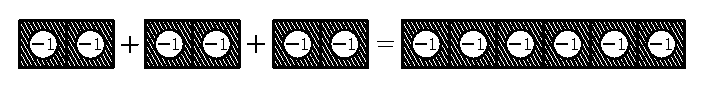
\includegraphics[scale=0.8]{src/figure/chap3/fig3-19.eps}\\
\end{figure}

ಚಿತ್ರದ ಸಹಾಯದಿಂದ, $[-2] + [-2] + [-2] = [-6]$

$\therefore [-2] \times [+3] = [-6]$

ಈಗ $[-] \times [+] = [-]$ ಆಗುತ್ತದೆ.

\noindent
{\textbf{\underline{ಉದಾ: 3 :}}} $[+2] \times [-3] = ?$

ಈ ಉದಾಹರಣೆಯಲ್ಲಿ ಎರಡನೇ ಸಂಖ್ಯೆ ಋಣ $[-]$ ಇರುವುದರಿಂದ ತೆಗೆಯುವುದು ಅಥವಾ ಕಡಿಮೆ ಮಾಡುವುದು. ಇಲ್ಲಿ ಬಿಲ್ಲೆಗಳು ಇಲ್ಲ. ಕಾರಣ ತಟಸ್ಥೀಕರಣ ನಿಯಮದಂತೆ, $[+1]$ರ 6 ಬಿಲ್ಲೆಗಳನ್ನು ಮತ್ತು $[-1]$ರ 6 ಬಿಲ್ಲೆಗಳನ್ನು ತೆಗೆದುಕೊಂಡು ಬಂದ ವ್ಯವಸ್ಥೆಯಲ್ಲಿ $[+1]$ರ ಎರಡು ಬಿಲ್ಲೆಗಳಂತೆ 3 ಸಲ ತೆಗೆಯಬೇಕು. ಆಗ ಉಳಿದ ಬೆಲೆಯು ಉದಾಹರಣೆಯ ಉತ್ತರವಾಗುತ್ತದೆ.
%~ \begin{figure}[H]
%~ \centering
%~ \includegraphics[scale=0.8]{src/figure/chap3/fig3-20a.eps}
%~ (ಚಿತ್ರ - 1)
%~ \end{figure}

ಚಿತ್ರದ ಸಹಾಯದಿಂದ $(+2) \times (-3) = [-6]$ ಇದನ್ನು ರೇಖಾಚಿತ್ರದ ಸಹಾಯದಿಂದ ತೋರಿಸಬಹುದು. 
\begin{figure}[H]
\centering
\includegraphics[scale=0.8]{src/figure/chap3/fig3-20b.eps}
\end{figure}

ಆಗ $[+2]\times [-3]=[-6]$ \ $\therefore$ \ $[+]\times [-]=[-]$ ಆಗುತ್ತದೆ.

\noindent
{\textbf{\underline{ಉದಾ: 4 :}}} $[-2] \times [-3] = ?$

ಈ ಉದಾಹರಣೆಯಲ್ಲಿ ಎರಡನೇ ಪದವು ಋಣ $(-)$ ಸಂಕೇತವನ್ನು ಹೊಂದಿದೆ.\break ಅಂದರೆ, $[-1]$ರ ಎರಡು ಬಿಲ್ಲೆಗಳಂತೆ 3ಸಲ ತೆಗೆಯಬೇಕು (ಕಡಿಮೆ ಮಾಡಬೇಕು) ಆದರೆ ಇಲ್ಲಿ ಬಿಲ್ಲೆಗಳು ಇರುವುದಿಲ್ಲ. ಕಾರಣ ತಟಸ್ಥೀಕರಣದ ನಿಯಮ ಪ್ರಕಾರ $[-1]$ರ 6 ಬಿಲ್ಲೆಗಳ ಜೊತೆಗೆ $[+1]$ರ 6 ಬಿಲ್ಲೆಗಳನ್ನು ತೆಗೆದುಕೊಂಡು. ಆಗ ಉಂಟಾಗುವ ವ್ಯವಸ್ಥೆಯಲ್ಲಿ $[-1]$ರ 2 ಬಿಲ್ಲೆಗಳಂತೆ 3 ಸಲ ತೆಗೆಯಬೇಕು. ಆಗ ಉಳಿಯುವ $[+1]$ರ 6 ಬಿಲ್ಲೆಗಳು ಈ ಉದಾ\break ಹರಣೆಯ ಉತ್ತರವಾಗಿರುತ್ತದೆ. ಇದನ್ನು ರೇಖಾಚಿತ್ರದಿಂದ ತೋರಿಸಿದೆ.
%~ \begin{figure}[H]
%~ \centering
%~ \includegraphics[scale=0.8]{src/figure/chap3/fig3-21a.eps}
%~ (ಚಿತ್ರ - 1)
%~ \end{figure}

%~ ಚಿತ್ರ -1ರ ಸಹಾಯದಿಂದ, $[-1]$ರ 2 ಬಿಲ್ಲೆಗಳನ್ನು 3 ಸಲ ತೆಗೆದಾಗ $[-6] + [+6] = [+6]$
%~ 
%~ $\therefore [-2] \times [-3] = [+6]$ ಅಂದರೆ, $(-) \times (-) = (+)$
%~ 
%~ ಇದನ್ನು ಚಿತ್ರ -2ರಲ್ಲಿ ರೇಖಾಚಿತ್ರದ ಸಹಾಯದಿಂದ ತೋರಿಸಬೇಕು. 
\begin{figure}[H]
\centering
\includegraphics[scale=0.8]{src/figure/chap3/fig3-21b.eps}
(ಚಿತ್ರ - 2)
\end{figure}

ಚಿತ್ರದ ಸಹಾಯದಿಂದ $[-2]\times [-3]=[+6]$ ಅಂದರೆ $[-]\times [-]=[+]$

\section{ಬಿಲ್ಲೆಗಳ ಸಹಾಯದಿಂದ ಅಪೂರ್ಣಂಕಗಳ ಗುಣಾಕಾರ :}\label{sec3.3}%% 3.3

ನಾವು ಪೂರ್ಣಂಕಗಳ ಗುಣಾಕಾರವನ್ನು ಬಿಲ್ಲೆಗಳ ಸಹಾಯದಿಂದ ತಿಳಿದುಕೊಂಡಿದ್ದೆವೆ. ಈಗ ಬಿಲ್ಲೆಗಳ ಸಹಾಯದಿಂದ ಅಪೂರ್ಣಂಕಗಳ ಗುಣಾಕಾರ ಕ್ರಿಯೆಯನ್ನು ತಿಳಿದುಕೊಳ್ಳುವುದು. ಇದಕ್ಕೆ ಕೆಳಗಿನ ಮಾಹಿತಿಗಳು ನಮಗೆ ತಿಳಿದಿರಬೇಕು.
\begin{figure}[H]
\centering
\includegraphics[scale=0.8]{src/figure/chap3/fig3-22.eps}
\end{figure}
ಒಂದು ಚೌರಸದ ಬೆಲೆ ಧನ ಬೆಲೆ $(+x^2)$ ಆಗಿದ್ದರೆ, ಅದರ ಬಾಹುಗಳು $(+x)$ ಅಥವಾ $(-x)$ ಇರಬಹುದು. ಆದರೆ ಚೌರಸದ ಬೆಲೆ. ಋಣಬೆಲೆ $(-x^2)$ ಆಗಿದ್ದರೆ, ಅದರ ಬಾಹುಗಳು ಒಂದು $(+x)$ ಇದ್ದರೆ, ಇನ್ನೊಂದು $(-x)$ ಅಥವಾ ಅದಕ್ಕೆ ವಿರೋಧವಾಗಿ ಇರುತ್ತವೆ.

\medskip
\noindent
{\textbf{\underline{ಅಪೂರ್ಣಂಕಗಳ ಗುಣಾಕಾರ :}}} 

\medskip
\noindent
{\textbf{\underline{ಉದಾ : }}} (1) $\frac{3}{5} \times \frac{3}{4} = ?$

\noindent
{\textbf{\underline{ವಿವರಣೆ :}}} ಈ ಉದಾಹರಣೆಯಲ್ಲಿ ಎರಡು ಅಪೂರ್ಣಂಕಗಳು ಧನ ಬೆಲೆ $(+)$ ಆಗಿದ್ದರಿಂದ $[+1]$ರ 20 ಬಿಲ್ಲೆಗಳನ್ನು ಉದ್ದ $+5$ ಮಾನಗಳು ಮತ್ತು ಅಗಲವು $+4$ ಮಾನಗಳು ಇರುವ ಆಯಾತ ಆಕಾರದಲ್ಲಿ ಜೋಡಿಸಬೇಕು. 
%~ \begin{figure}[H]
%~ \centering
%~ \includegraphics[scale=0.8]{src/figure/chap3/fig3-23a.eps}
%~ \end{figure}

ಈಗ ಆಯತದ ಉದ್ದ $(+5)$ ಮಾನವಾದರೆ ಅಗಲವು $(+4)$ ಮಾನಗಳಾಗುತ್ತವೆ.\break ಹಾಗೂ ಈ ಆಯತದ ವಿಸ್ತೀರ್ಣವು 1ಚ.ಮಾನ ಇರಲಿ, ಈ ಆಯತದ ಉದ್ದದಲ್ಲಿ $[+3]$ ಮಾನವನ್ನು ತೆಗೆದುಕೊಂಡರೆ, ಅದು $\left[+\frac{3}{5}\right]$ ಆಗುತ್ತದೆ. ಮತ್ತು ಅಗಲದಲ್ಲಿ $[+3]$ಮಾನವನ್ನು ತೆಗೆದುಕೊಂಡರೆ ಅದು $\left[+\frac{3}{4}\right]$ ಆಗುತ್ತದೆ. ಈಗ ಈ ತುಂಡಿನ ವಿಸ್ತೀರ್ಣವು $\left[\left(+ \frac{3}{5}\right) \times \left(+\frac{3}{4}\right)\right]$ ಆಗುವುದು. 

ಒಟ್ಟು ವಿಸ್ತೀರ್ಣವು $\left[+\frac{9}{20}\right]$ ಆಗುತ್ತದೆ.

$\therefore \left[\left(+\frac{3}{5}\right) \times \left(+\frac{3}{4}\right) \right] = \left[+\frac{9}{20} \right]$

ಜೋಡನೆಯನ್ನು ಕೆಳಗಿನ ಚಿತ್ರದಲ್ಲಿ ತೋರಿಸಂತೆ ತೋರಿಸಬಹುದು. 
\begin{figure}[H]
\centering
\includegraphics[scale=0.8]{src/figure/chap3/fig3-23b.eps}
\end{figure}
\begin{align*}
ABCD ~\text{ವಿಸ್ತೀರ್ಣ}  & = 20 ~\text{ಚ. ಮಾನಗಳು}\\
AEFG ~\text{ವಿಸ್ತೀರ್ಣ} & = 9 ~\text{ಚ. ಮಾನಗಳು}\\
\therefore ~\text{ತುಂಡಿನ ವಿಸ್ತೀರ್ಣ} & = \left[+\dfrac{9}{20}\right]\\
\therefore \ \left[+\frac{3}{5}\right]\times \left[+\frac{3}{4}\right] &=\left[\frac{9}{20}\right]
\end{align*}

\noindent
{\textbf{\underline{ಉದಾ: 2 :}}} $\left(+\frac{3}{4} \right) \times \left(+\frac{1}{2} \right) = ?$

\noindent
{\textbf{\underline{ವಿವರಣೆ :}}} ಈ ಉದಾಹರಣೆಯಲ್ಲಿ ಎರಡು ಬೆಲೆಗಳು ಧನ ಬೆಲೆ $(+)$ ಆಗಿದ್ದರಿಂದ $[+1]$ರ '8' ಬಿಲ್ಲೆಗಳನ್ನು ಉದ್ದ $(+4)$ ಮಾನಗಳು ಮತ್ತು ಅಗಲವು $(+2)$ ಮಾನಗಳು ಇರುವಂತೆ ಜೋಡಿಸಿದಾಗ ಆಯತದ ವಿಸ್ತೀರ್ಣವು $(+8)$ ಚ. ಮಾನಗಳಾಗುತ್ತದೆ. 
%~ \begin{figure}[H]
%~ \centering
%~ \includegraphics[scale=0.8]{src/figure/chap3/fig3-24a.eps}
%~ \end{figure}

ಈ ಬೆಲೆಯು 1ಚ. ಮಾನವಾಗಿರಲಿ, ಈ ಆಯತದ ಉದ್ದದಲ್ಲಿ $(+3)$ ಮಾನಗಳನ್ನು\break  ತೆಗೆದುಕೊಂಡರೆ ಅದು $\left(+\frac{3}{4} \right)$ ಮಾನಗಳು ಆಗುತ್ತದೆ. ಮತ್ತು ಅಗಲದಲ್ಲಿ $(+1)$ ಮಾನವನ್ನು ತೆಗೆದುಕೊಂಡರೆ ಅದು $\left(+\frac{1}{2}\right)$ ಮಾನ ಆಗುತ್ತದೆ. ಈಗ $\left(+\frac{3}{4} \right)$ ಮಾನಗಳು ಉದ್ದ ಮತ್ತು $\left(+\frac{1}{2} \right)$ ಮಾನಗಳು ಅಗಲ ಇರುವ ಒಂದು ತುಂಡು ಸಿಗುತ್ತದೆ. ಈ ತುಂಡಿನ ವಿಸ್ತೀರ್ಣವು $\left[\left(+\frac{3}{4}\right) \times \left(+\frac{1}{2}\right) \right]$ ಆಗುವುದು. 
  
ಈ ವಿಸ್ತೀರ್ಣವು ಒಟ್ಟು ವಿಸ್ತೀರ್ಣದ $(+8)$ಚ. ಮಾನಗಳು $\left[+\frac{3}{8}\right]$ ಚ. ಮಾನಗಳಾಗುತ್ತದೆ.
  
$\therefore \left[\left(+\frac{3}{4}\right) \times \left(+\frac{1}{2}\right) \right] = \left[+\frac{3}{8}\right]$ ಇದನ್ನು ರೇಖಾಚಿತ್ರದ ಸಹಾಯದಿಂದ ವಿವರಿಸ\-ಬಹುದು. 
\begin{figure}[H]
\centering
\includegraphics[scale=0.8]{src/figure/chap3/fig3-24b.eps}
\end{figure}
\vskip -1.2cm
\begin{align*}
\text{ಚಿತ್ರದಲ್ಲಿ}~ ABCD~ \text{ವಿಸ್ತೀರ್ಣ} & = (+8)~ \text{ಚ. ಮಾನಗಳು.}\\
\text{ಮತ್ತು}~ AEFG~ \text{ವಿಸ್ತೀರ್ಣ} & = (+3)~ \text{ಚ. ಮಾನಗಳು.}
\end{align*}

$\therefore AEFG$ ತುಂಡಿನ ವಿಸ್ತೀರ್ಣವು $\left[+\frac{3}{8}\right]$ ಚ. ಮಾನಗಳಾಗುತ್ತದೆ. 

$\therefore \left[\left(+\frac{3}{4}\right) \times \left(+\frac{1}{2}\right)\right] = \left[+\frac{3}{8}\right]$

%%\vfill%%%%\eject

\noindent
{\textbf{\underline{ಉದಾ : 3:}}} $\left(+\frac{3}{4} \right) \times \left(-\frac{2}{3} \right)$

\noindent
{\textbf{\underline{ವಿವರಣೆ :}}} ಈ ಉದಾಹರಣೆಯಲ್ಲಿ ಒಂದು ಋಣ ಬೆಲೆ $(-)$ ಮತ್ತು ಒಂದು ಧನ ಬೆಲೆ $(+)$ ಇರುವುದರಿಂದ $[-1]$ರ 12 ಬಿಲ್ಲೆಗಳನ್ನು ಉಪಯೋಗಿಸಿ $(+4)$ ಮಾನಗಳು ಉದ್ದ ಮತ್ತು $(+3)$ ಮಾನಗಳು ಅಗಲವಿರುವ ಒಂದು ಆಯತವನ್ನು ರಚಿಸಬೇಕು. ಈ ಆಯತದ \hbox{ವಿಸ್ತೀರ್ಣವು} $[+12]$ ಚ.ಮಾನಗಳಾಗುತ್ತವೆ.
%~ \begin{figure}[H]
%~ \centering
%~ \includegraphics[scale=0.8]{src/figure/chap3/fig3-25a.eps}
%~ \end{figure}

ಈ ವಿಸ್ತೀರ್ಣವು 1 ಚ. ಮಾನ ಎಂದು ತಿಳಿದು ಕೊಳ್ಳುವಾ. ಇಲ್ಲಿ ಉದ್ದವು ಧನ $(+)$ ಅಪೂರ್ಣಂಕ ಮತ್ತು ಅಗಲವು ಋಣ $(-)$ ಅಪೂರ್ಣಂಕವಾಗಿರುತ್ತದೆ.

ಈಗ ಉದ್ದದಲ್ಲಿ 3 ಮಾನಗಳನ್ನು ತೆಗೆದುಕೊಂಡಾಗ ಅದು $\left(+\frac{3}{4} \right)$ ಆಗುವುದು ಮತ್ತು ಅಗಲದಲ್ಲಿ 2 ಮಾನಗಳನ್ನು ತೆಗೆದುಕೊಂಡಾಗ ಅದು $\left(-\frac{2}{3} \right)$ ಆಗುವುದು. ಆದ್ದರಿಂದ ಉದ್ದ $\left(+\frac{3}{4} \right)$ ಮತ್ತು ಅಗಲವು $\left(-\frac{2}{3} \right)$ ಇರುವ ಆಯತಾಕಾರದ ತುಂಡಿನ ವಿಸ್ತೀರ್ಣವು $\left[\left(+\frac{3}{4} \right) \times \left(-\frac{2}{3} \right)\right]$ ಆಗುತ್ತದೆ. ಇದು $\left[-\frac{6}{12}\right]$ಗೆ ಸಮವಾಗುತ್ತದೆ.
$$
\therefore \left[\left(+\frac{3}{4}\right) \times \left(-\frac{2}{3}\right)\right] = \left[-\frac{6}{12}\right] = \left[\frac{1}{2} \right]
$$

ಇದನ್ನು ಕೆಳಗಿನಂತೆ ರೇಖಾಚಿತ್ರದಿಂದ ಸೂಚಿಸಬಹುದು. 
\begin{figure}[H]
\centering
\includegraphics[scale=0.8]{src/figure/chap3/fig3-25b.eps}
\end{figure}
\begin{align*}
\text{ಚಿತ್ರದಲ್ಲಿ}~ ABCD ~\text{ವಿಸ್ತೀರ್ಣ} & = 12~ \text{ಚ. ಮಾನಗಳು.}\\
AEFG~ \text{ವಿಸ್ತೀರ್ಣ} & = -6~ \text{ಚ. ಮಾನಗಳು.}\\
\therefore~ \text{ತುಂಡಿನ ವಿಸ್ತೀರ್ಣ} &  = \left[\frac{-6}{12}\right] = \left(-\frac{6}{12} \right)=\left[-\frac{1}{2}\right]\\
\therefore~ \left[+ \frac{3}{4}\right] \times \left[-\frac{2}{3}\right] & = \left[- \frac{1}{2}\right]
\end{align*}

\noindent
{\textbf{\underline{ಉದಾ : 4 :}}} $\left[\left(-\frac{5}{6}\right) \times \left(+\frac{2}{3}\right) \right] = ?$
%~ \begin{figure}[H]
%~ \centering
%~ \includegraphics[scale=0.8]{src/figure/chap3/fig3-26a.eps}
%~ \end{figure}

\noindent
{\textbf{\underline{ವಿವರಣೆ :}}} ಅಪೂರ್ಣಂಕಗಳಲ್ಲಿ ಒಂದು ಧನ $(+)$ ಸಂಖ್ಯೆಯಾಗಿದ್ದು ಇನ್ನೊಂದು ಋಣ $(-1)$ ಅಪೂರ್ಣಂಕವಾಗಿರುವುದರಿಂದ ಇಲ್ಲಿ $(-1)$ರ ಬಿಲ್ಲೆಗಳನ್ನು ಉಪಯೋಗಿಸಬೇಕು. ಅಪೂರ್ಣಂಕಗಳ ಛೇದಗಳು 6 ಮತ್ತು 3 ಇರುವುದರಿಂದ 18 ಸಂಖ್ಯೆಯಲ್ಲಿ $[-1]$ರ ಬಿಲ್ಲೆಗಳನ್ನು ಉದ್ದ 6 ಮಾನಗಳು ಮತ್ತು ಅಗಲವು 3 ಮಾನಗಳು ಇರುವಂತೆ ಆಯತ ಆಕಾರದಲ್ಲಿ ಜೋಡಿಸಬೇಕು. ಇದರ ವಿಸ್ತೀರ್ಣವು 1ಚ. ಮಾನಗಳು ಇರಲಿ, ಈಗ ಉದ್ದದಲ್ಲಿ 5 ಮಾನಗಳನ್ನು ತೆಗೆದುಕೊಂಡರೆ ಅದರ ಬೆಲೆ $\left(-\frac{5}{6} \right)$ ಆಗುವುದು. ಮತ್ತು ಅಗಲದಲ್ಲಿ 2 ಮಾನಗಳನ್ನು ತೆಗೆದುಕೊಂಡರೆ ಅದರ ಬೆಲೆ $\left(+\frac{2}{3}\right)$ ಆಗುವುದು. ಇಲ್ಲಿ ಉದ್ದ $\left(-\frac{5}{6}\right)$ ಮತ್ತು ಅಗಲ $\left(+\frac{2}{3} \right)$ ಇರುವ ಒಂದು ತುಂಡು ದೊರಕುತ್ತದೆ. ಅದರಲ್ಲಿ $(-1)$ರ 10 ಬಿಲ್ಲೆಗಳು ಇರುತ್ತವೆ. ಅಂದರೆ ಆ ತುಂಡಿನ ವಿಸ್ತೀರ್ಣವು $\left(\frac{-10}{18}\right)$ ಆಗುತ್ತದೆ.
$$
\therefore~ \left[\left(-\frac{5}{6}\right) \times \left(+ \frac{2}{3}\right) \right] = \left[-\frac{10}{18}\right]=\left[-\frac{5}{9}\right] \text{ ಆಗುವುದು.}
$$

%%%%\eject

ಇದನ್ನು ಕೆಳಗಿನಂತೆ ರೇಖಾ ಚಿತ್ರದಲ್ಲಿ ತೋರಿಸಬೇಕು.
\begin{figure}[H]
\centering
\includegraphics[scale=0.8]{src/figure/chap3/fig3-26b.eps}
\end{figure}
\begin{align*}
\text{ಚಿತ್ರದಲ್ಲಿ}~ ABCD~ \text{ವಿಸ್ತೀರ್ಣ} & = 18\\
\text{ಮತ್ತು}~ AEFG~ \text{ವಿಸ್ತೀರ್ಣ} & = -10\\
\therefore~ \text{ತುಂಡಿನ ವಿಸ್ತೀರ್ಣ} & = \left(\frac{10}{-18} \right) = \left(-\frac{10}{18} \right)=\left(-\frac{5}{9}\right)
\end{align*}


\noindent
{\textbf{\underline{ಉದಾ : 5 :}}} $\left[\left(-\frac{3}{4} \right) \times \left(-\frac{3}{5} \right) \right] = ?$
%~ \begin{figure}[H]
%~ \centering
%~ \includegraphics[scale=0.8]{src/figure/chap3/fig3-27a.eps}
%~ \end{figure}

\noindent
{\textbf{\underline{ವಿವರಣೆ :}}} ಎರಡು ಅಪೂರ್ಣಂಕಗಳು ಋಣ $(-)$ ಬೆಲೆಗಳನ್ನು ಹೊಂದಿವೆ. ಆದ್ದರಿಂದ ಉದ್ದ ಅಗಲಗಳು. ಋಣ ಬೆಲೆಯನ್ನು ಹೊಂದಿರುವುದರಿಂದ ಈ ಉದಾಹರಣೆಯಲ್ಲಿ ಧನ $(+)$ ಬಿಲ್ಲೆಗಳನ್ನು ಉಪಯೋಗಿಸಬೇಕು. ಎರಡು ಅಪೂರ್ಣಂಕಗಳ ಛೇದಗಳು 4 ಮತ್ತು 5 ಇರುವುದರಿಂದ $(+1)$ರ 20 ಬಿಲ್ಲೆಗಳನ್ನು ಚಿತ್ರದಲ್ಲಿ ತೋರಿಸಿದಂತೆ ಉದ್ದ 5 ಮಾನಗಳು ಮತ್ತು ಅಗಲವು 4 ಮಾನಗಳು ಇರುವ ಹಾಗೆ ಬಿಲ್ಲೆಗಳನ್ನು ಆಯಾತ ಆಕಾರದಲ್ಲಿ ಜೋಡಿಸಬೇಕು. ಇದರ ವಿಸ್ತೀರ್ಣವು 20 ಚ. ಮಾನಗಳಾಗುತ್ತದೆ. ಇದು 1 ಚ. ಮಾನವೆಂದು ತಿಳಿದುಕೊಳ್ಳ\break ಬೇಕು. 

ಈಗ ಉದ್ದದಲ್ಲಿ $(-3)$ ಮಾನಗಳನ್ನು ತೆಗೆದುಕೊಂಡರೆ, ಅದು $\left(-\frac{3}{5}\right)$ ಆಗುವುದು. ಅದರಂತೆ ಅಗಲದಲ್ಲಿ $(-3)$ ಮಾನಗಳನ್ನು ತೆಗೆದುಕೊಂಡರೆ ಅದು $\left(-\frac{3}{4} \right)$ ಆಗುವುದು. ಆದ್ದರಿಂದ ಇಲ್ಲಿ ಉಂಟಾಗುವ ಆಯತಾಕಾರದ ತುಂಡಿನ ಉದ್ದ $\left(-\frac{3}{5} \right)$ ಮತ್ತು ಅಗಲವು $\left(-\frac{3}{4}\right)$ ಆಗುವುದರಿಂದ ಇದರ ವಿಸ್ತೀರ್ಣವು $(+1)$ ಬಿಲ್ಲೆಗಳು '9' ಸೇರಿದ ಬೆಲೆಗೆ ಸಮ\-ವಿರುತ್ತದೆ.

ಅಂದರೆ ಇದು 20ರಲ್ಲಿ 9 ಬೆಲೆಗೆ ಸಮವಾಗಿದೆ. ಆಗ $\left(+\frac{9}{20} \right)$ ಆಗುತ್ತದೆ. 
$$
\therefore~ \left[\left(-\frac{3}{5}\right) \times \left(-\frac{3}{4}\right) \right] = \left[+\frac{9}{20} \right]
$$

ಇದನ್ನು ಕೆಳಗಿನಂತೆ ರೇಖಾಚಿತ್ರದ ಮೂಲಕ ತೋರಿಸಬಹುದು. 
\begin{figure}[H]
\centering
\includegraphics[scale=0.7]{src/figure/chap3/fig3-27b.eps}
\end{figure}
\vskip -1.2cm
\begin{align*}
\text{ಚಿತ್ರದಲ್ಲಿ}~ ABCD ~\text{ಯ ವಿಸ್ತೀರ್ಣ} & = 20~ \text{ಚ. ಮಾನಗಳು}\\
\text{ಮತ್ತು}~ AEFG ~\text{ಯ ವಿಸ್ತೀರ್ಣ} & = 9~ \text{ಚ. ಮಾನಗಳು}\\
\therefore~ \text{ತುಂಡಿನ ವಿಸ್ತೀರ್ಣ} & = \left(+\frac{9}{20} \right) ಚ. ಮಾನಗಳು\\
\therefore~ \left[\left(-\frac{3}{5}\right) \times \left(-\frac{3}{4}\right) \right] & = \left[+ \frac{9}{20} \right]
\end{align*}

\noindent
{\textbf{\underline{ಉದಾ : 6 :}}} $\left[\left(-\frac{3}{4}\right) \times \left(-\frac{1}{2}\right) \right] = ?$
%~ \begin{figure}[H]
%~ \centering
%~ \includegraphics[scale=0.8]{src/figure/chap3/fig3-28a.eps}
%~ \end{figure}

\noindent
{\textbf{\underline{ವಿವರಣೆ :}}} ಎರಡು ಅಪೂರ್ಣಂಕಗಳು ಋಣ $(-)$ ಚಿಹ್ನೆಯನ್ನು ಹೊಂದಿರುವುದರಿಂದ $(+1)$ರ ಧನ ಬಿಲ್ಲೆಗಳನ್ನು ತೆಗೆದುಕೊಳ್ಳಬೇಕು. ಈಗ $(+1)$ರ 8 ಬಿಲ್ಲೆಗಳನ್ನು ತೆಗೆದು\-ಕೊಂಡು ಉದ್ದ 4 ಮಾನಗಳಲ್ಲಿ ಮತ್ತು ಅಗಲವು 2 ಮಾನಗಳಲ್ಲಿ ಇರುವಂತೆ ಆಯತ ಆಕಾರದಲ್ಲಿ\break  ಜೋಡಿಸಬೇಕು. ಇದರ ವಿಸ್ತೀರ್ಣವು 8 ಚ. ಮಾನಗಳಾಗುತ್ತದೆ. 

ಈಗ ಉದ್ದದಲ್ಲಿ 3 ಮಾನಗಳನ್ನು ತೆಗೆದುಕೊಂಡರೆ ಅದು $\left(-\frac{3}{4}\right)$ ಆದರೆ, ಅಗಲದಲ್ಲಿ 1 ಮಾನವನ್ನು ತೆಗೆದುಕೊಂಡರೆ $\left(-\frac{1}{2} \right)$ ಆಗುತ್ತದೆ. ಆದ್ದರಿಂದ ಈ ತುಂಡಿನ ವಿಸ್ತೀರ್ಣವು $\left[\left(-\frac{3}{4}\right) \times \left(-\frac{1}{2}\right) \right]$ಕ್ಕೆ ಸಮವಾಗುತ್ತದೆ. ಇದು $\left(+\frac{3}{8}\right)$ಕ್ಕೆ ಸರಿ ಹೊಂದುತ್ತದೆ. 
$$
\therefore~ \left[\left(-\frac{3}{4}\right) \times \left(-\frac{1}{2}\right) \right] = \left[+ \frac{3}{8} \right]
$$

ಇದನ್ನು ರೇಖಾಚಿತ್ರದ ಮೂಲತ ಕೆಳಗಿನಂತೆ ತೋರಿಸಬೇಕು. 
\begin{figure}[H]
\centering
\includegraphics[scale=0.8]{src/figure/chap3/fig3-28b.eps}
\end{figure}
\begin{align*}
\text{ಚಿತ್ರದಲ್ಲಿ}~ ABCD ~\text{ವಿಸ್ತೀರ್ಣ} & = +8~ \text{ಚ. ಮಾನಗಳು.}\\
\text{ಮತ್ತು}~ AEFG ~\text{ವಿಸ್ತೀರ್ಣ} & = +3~ \text{ಚ. ಮಾನಗಳು.}\\
\therefore~ \text{ತುಂಡಿನ ವಿಸ್ತೀರ್ಣವು} & = \left(+\frac{3}{8} \right) \text{ಚ. ಮಾನಗಳು.}\\
\therefore~ \left[\left(-\frac{3}{4}\right) \times \left(-\frac{1}{2}\right) \right] & = \left[+\frac{3}{8}\right]
\end{align*}

\section{"ಬಿಲ್ಲೆಗಳ ಅನ್ವಯಗಳು"}\label{sec3.4}%% 3.4

\section*{ಬೀಜ ಪದಗಳ ಗುಣಾಕಾರ ಅಥವಾ ಗುಣಲಬ್ಧ ಕಂಡು ಹಿಡಿಯುವುದು.}

ಎರಡು ಬೀಜ ಪದಗಳ ಗುಣಲಬ್ಧ ಕಂಡು ಹಿಡಿಯಬೇಕಾದರೆ,
\smallskip
\smallskip
\begin{itemize}
\item [(a)] ಬೀಜ ಪದಗಳಲ್ಲಿರುವ ಬೀಜಾಕ್ಷರ ತಕ್ಕಂತೆ ಬಿಲ್ಲೆಗಳನ್ನು ಆಯ್ಕೆ ಮಾಡಿಕೊಳ್ಳಬೇಕು.

\smallskip

\begin{tabular}{lll}
ಉದಾಹರಣೆಗಾಗಿ, & 'x' ಬೀಜಾಕ್ಷರ ಇದ್ದರೆ, & $\pm x^2$ ಮತ್ತು $\pm x$ ಬಿಲ್ಲೆಗಳು.\\[0.1cm]
& 'y' ಬೀಜಾಕ್ಷರ ಇದ್ದರೆ, & $\pm y^2$ ಮತ್ತು $\pm y$ ಬಿಲ್ಲೆಗಳು.\\[0.1cm]
& 'a' ಬೀಜಾಕ್ಷರ ಇದ್ದರೆ, & $\pm a^2$ ಮತ್ತು $\pm a$ ಬಿಲ್ಲೆಗಳು.\\[0.1cm]
& ಸಂಖ್ಯೆಗಳು ಇದ್ದರೆ, & $\pm 1$ ಬಿಲ್ಲೆಗಳು.  
\end{tabular}

\medskip

\item [(b)] ಎರಡು ಬೀಜ ಪದಗಳಲ್ಲಿ ಒಂದನ್ನು ಆಯತ/ಚೌರಸದ ಉದ್ದವೆಂದು, ಇನ್ನೊಂದನ್ನು ಅಗಲವೆಂದು ತಿಳಿದುಕೊಳ್ಳಬೇಕು. 

\medskip

\item [(c)] ಉದ್ದ - ಅಗಲಗಳ ಬೀಜ ಪದಗಳು ಬರುವಂತೆ, ಬಿಲ್ಲೆಗಳನ್ನು ಪರಸ್ಪರ ಲಂಬವಿರುವ ox ಮತ್ತು oy ಅಕ್ಷಗಳಗುಂಟ ಜೋಡಿಸಬೇಕು. 

\medskip

\item [(d)] ಉದ್ದ - ಅಗಲಗಳ ಸರಿ ಆದ ನಂತರ ಆಯತ/ಚೌರಸನ್ನು ಪೂರ್ಣಗೊಳಿಸಬೇಕು. 

\medskip

\item [(e)] ಆಗ ಉಂಟಾಗುವ ಎಲ್ಲ ಬಿಲ್ಲೆಗಳ ಮೊತ್ತವೇ ಆ ಎರಡು ಬೀಜ ಪದಗಳ ಗುಣಲಬ್ಧ\break ವಾಗಿರುತ್ತದೆ.
\end{itemize}

\medskip
\noindent
{\textbf{\underline{ಸೂಚನೆ :}}} ಮೇಲಿನಂತೆ ಪ್ರಯೋಗ ಮಾಡಬೇಕಾದರೆ, ಫೇನಲ್ ಕ್ಲಾತ್ ಅಂಟಿಸಿದ ಬೋರ್ಡ್ ಮತ್ತು ಉಸಿಕಿನ ಹಾಳೆ ಅಂಟಿಸಿದ ಕಾರ್ಡ್ ಶೀಟ್ ಕಾಗದದ ಬಿಲ್ಲೆಗಳನ್ನು ಉಪಯೋಗಿಸ\-ಬೇಕು. 

\smallskip

ಇದು ಮಕ್ಕಳಿಗೆ ಒಂದು ಚಟುವಟಿಕೆಯಾಗುವುದರಿಂದ ಆಸಕ್ತಿಯಿಂದ ಭಾಗವಹಿಸಿ ಗಣಿತದ ಬಗ್ಗೆ ಸರಿಯಾಗಿ ತಿಳಿದುಕೊಳ್ಳುತ್ತಾರೆ. ಅಲ್ಲದೇ ಜೋಡಿಸಿದ ಬಿಲ್ಲೆಗಳ ರೇಖಾಚಿತ್ರವನ್ನು ನಾವು ಕಾಗದದಲ್ಲಿ ಎಳೆಯಬೇಕು. ಧನಾತ್ಮಕ ಬಿಲ್ಲೆಗಳನ್ನು ಖಾಲಿ ಸ್ಥಳದಿಂದ, ಋಣಾತ್ಮಕ ಬಿಲ್ಲೆಗಳನ್ನು ಗೆರೆ ತುಂಬಿದ ಸ್ಥಳದಿಂದ ಗುರುತಿಸಬೇಕು.

\section*{ಎರಡು ಏಕ ಪದಗಳ ಗುಣಲಬ್ಧ ಕಂಡು-ಕೊಳ್ಳುವುದು.}

\noindent
{\textbf{\underline{ಉದಾ: (1)}}} $a \times 3a = ?$

ಉದಾಹರಣೆಗೆ ತಕ್ಕಂತೆ ರೇಖಾಚಿತ್ರ ತೆಗೆಯಬೇಕು.
\begin{figure}[H]
\centering
\includegraphics[scale=0.9]{src/figure/chap3/fig3-29a.eps}
\end{figure}

\noindent
{\textbf{\underline{ಹಂತಗಳು :}}}

\begin{itemize}
\item [(1)] ಚಿತ್ರದಲ್ಲಿ ತೋರಿಸಿದಂತೆ ಉದ್ದ = a, ಅಗಲ = 3a ಆಗುವಂತೆ ox ಮತ್ತು oy ಅಕ್ಷಗಳಗುಂಟ ಬಿಲ್ಲೆಗಳನ್ನು ಜೋಡಿಸಬೇಕು. 
\item [(2)] ಇದು ಒಂದು ಪೂರ್ಣ ಆಯತವಾಗಿದ್ದರಿಂದ ಎಲ ಬಿಲ್ಲೆಗಳ ಒಟ್ಟು ಮೊತ್ತವೇ\break ಆಯತದ ವಿಸ್ತೀರ್ಣವಾಗಿರುತ್ತದೆ. ವಿಸ್ತೀರ್ಣ = $3a^2$
\item [(3)] ಆಯತದ ವಿಸ್ತೀರ್ಣವು ಅದರ ಉದ್ದ ಅಗಲಗಳ ಗುಣಲಬ್ಧಕ್ಕೆ ಸಮವಾಗಿದೆ. 
\begin{gather*}
\therefore~ A = lb \\
\therefore~ 3a^2 = 3a \times a\\
\therefore~ 3a \times a = 3a^2
\end{gather*}

%\item [(4)] ಚಿತ್ರ -2ರಲ್ಲಿ ತೋರಿಸಿದಂತೆ ರೇಖಾಚಿತ್ರದಿಂದ ತೋರಿಸಬೇಕು. 
\end{itemize}

\medskip
\noindent
{\textbf{\underline{ಉದಾ : (2) :}}} $2x \times 3x = ?$

ಬಿಲ್ಲೆಗಳನ್ನು ಉಪಯೋಗಿಸಿ ಕೆಳಗಿನಂತೆ ರೇಖಾಚಿತ್ರವನ್ನು ರಚಿಸಬೇಕು.
\begin{figure}[H]
\centering
\includegraphics[scale=0.9]{src/figure/chap3/fig3-29b.eps}
\end{figure}

\noindent
{\textbf{\underline{ಹಂತಗಳು : }}} ರೇಖಾಚಿತ್ರದ ಸಹಾಯದಿಂದ
\begin{itemize}
\item [(1)] ಚಿತ್ರ -1ರಲ್ಲಿ ತೋರಿಸಿದಂತೆ ಉದ್ದ = 2x, ಅಗಲ = 3x ಆಗುವಂತೆ ox ಮತ್ತು oy ಅಕ್ಷಗಳಗುಂಟ ಬಿಲ್ಲೆಗಳನ್ನು ಜೋಡಿಸಬೇಕು. 

\item [(2)] ಇದು ಒಂದು ಪೂರ್ಣ ಆಯತವಾಗಿದ್ದರಿಂದ ಎಲ್ಲ ಬಿಲ್ಲೆಗಳ ಒಟ್ಟು ಮೊತ್ತವೇ\break ಆಯತದ ವಿಸ್ತೀರ್ಣವಾಗಿದೆ. ವಿಸ್ತೀರ್ಣ $= A = 6x^2$

\item [(3)] ಆಯತದ ವಿಸ್ತೀರ್ಣವು ಅದರ ಉದ್ದ $-$ ಅಗಲಗಳ ಗುಣಲಬ್ಧಕ್ಕೆ ಸಮವಾಗಿದೆ.
\begin{align*}
\therefore~ A & = lb\\
6x^2 & = 2x \times 3x\\
\therefore~ 2x \times 3x & = 6x^2
\end{align*}

%\item [(4)] ಚಿತ್ರೆ -2ರಲ್ಲಿ ತೋರಿಸಿದಂತೆ ರೇಖಾಚಿತ್ರದಿಂದ ತೋರಿಸಬೇಕು.
\end{itemize}

\section{ಒಂದು ಏಕ ಪದದಿಂದ ಒಂದು ಬೀಜೋಕ್ತಿಯನ್ನು ಗುಣಿಸುವುದು.}\label{sec3.5}%% 3.5

\noindent
{\textbf{\underline{ಉದಾ : (1)}}} $2x (x-3) = ?$

ಬಿಲ್ಲೆಗಳ ಸಹಾಯದಿಂದ ರೇಖಾಚಿತ್ರವನ್ನು ರಚಿಸಬೇಕು.
\begin{figure}[H]
\centering
\includegraphics[scale=0.8]{src/figure/chap3/fig3-30a.eps}
\end{figure}
ಚಿತ್ರದ ವಿವರಣೆ.

\noindent
{\textbf{\underline{ಹಂತಗಳು :}}} 
\begin{itemize}
\item [(1)] $l = 2x$, $b = (x-3)$ ಆಗುವಂತೆ ಚಿತ್ರದಲ್ಲಿ ತೋರಿಸಿದಂತೆ ಬಿಲ್ಲೆಗಳನ್ನು ಜೋಡಿಸಬೇಕು. 
\item [(2)] ಜೋಡಣೆ ಆಯತ ಆಕಾರವನ್ನು ಹೊಂದಿದಾಗ, ಎಲ್ಲ ಬಿಲ್ಲೆಗಳ ವಿಸ್ತೀರ್ಣವು ಒಟ್ಟು ಆಯತದ ವಿಸ್ತೀರ್ಣವಾಗುತ್ತದೆ. ವಿಸ್ತೀರ್ಣ = $2x^2 - 6x$
\item [(3)] ಆಯತದ ವಿಸ್ತೀರ್ಣವು ಅದರ ಉದ್ದ - ಅಗಲಗಳ ಗುಣಲಬ್ಧವಾಗಿರುತ್ತದೆ. 

\begin{tabular}{ll}
$\therefore$ & $lb = A$\\
$\therefore$ & $2x \times (x - 3) = (2x^2 - 6x)$
\end{tabular}

%\item [(4)] ಚಿತ್ರ -2ರಲ್ಲಿ ತೋರಿಸಿದಂತೆ ರೇಖಾಚಿತ್ರದಿಂದ ಗುರುತಿಸಬೇಕು. 
\end{itemize}

\eject

\noindent
{\textbf{\underline{ಉದಾ : 2 :}}} $m \times (m - 2) = ?$

ಬಿಲ್ಲೆಗಳ ಸಹಾಯದಿಂದ ರೇಖಾಚಿತ್ರವನ್ನು ರಚಿಸಬೇಕು.
\begin{figure}[H]
\centering
\includegraphics[scale=0.8]{src/figure/chap3/fig3-30b.eps}
\end{figure}
~
\vskip -0.5cm
ಚಿತ್ರದ ಸಹಾಯದಿಂದ

\noindent
{\textbf{\underline{ಹಂತಗಳು :}}} 
\begin{itemize}
\item [(1)] ಚಿತ್ರದಲ್ಲಿ ತೋರಿಸಿದಂತೆ ಉದ್ದ = $m$, ಅಗಲ = $(m - 2)$ ಆಗುವಂತೆ ox ಮತ್ತು oy ಗಳಗುಂಟ ಬಿಲ್ಲೆಗಳನ್ನು ಜೋಡಿಸಿ, ಆಯತವನ್ನು ಪೂರ್ಣಗೊಳಿಸಬೇಕು.
\item [(2)] ಆಯತದ ಎಲ್ಲ ಬಿಲ್ಲೆಗಳ ಒಟ್ಟು ಮೊತ್ತವೆ ಆಯತದ ವಿಸ್ತೀರ್ಣವಾಗಿದೆ. ಆಯತದ ವಿಸ್ತೀರ್ಣ $= (m^2 - 2m)$
\item [(3)] ಆಯತದ ವಿಸ್ತೀರ್ಣವು ಆಯತದ ಉದ್ದ ಅಗಲಗಳ ಗುಣಲಬ್ಧಕ್ಕೆ ಸಮವಿರುತ್ತದೆ.
\begin{gather*}
lb = A\\
\therefore~ m \times (m - 2) = (m^2 - 2m)
\end{gather*}

%\item [(4)] ಚಿತ್ರ -2ರಲ್ಲಿ ತೋರಿಸಿದಂತೆ ಇದನ್ನು ರೇಖಾ ಚಿತ್ರದ ಮೂಲಕ ತೋರಿಸಬೇಕು.
\end{itemize}

\section{ಬಿಲ್ಲೆಗಳ ಸಹಾಯದಿಂದ ಎರಡು ದ್ವಿಪದಗಳ ಗುಣಲಬ್ಧ ಕಂಡು ಹಿಡಿಯು\break ವುದು.}\label{sec3.6}%%3.6

\noindent
{\textbf{\underline{ಉದಾ : 1 :}}} $(x + 2)(x - 1) = ?$

ಬಿಲ್ಲೆಗಳ ಸಹಾಯದಿಂದ ರೇಖಾಚಿತ್ರವನ್ನು ರಚಿಸಬೇಕು.
\begin{figure}[H]
\centering
\includegraphics[scale=0.8]{src/figure/chap3/fig3-31a.eps}
\end{figure}
~
\vskip -0.5cm
ಚಿತ್ರದ ಸಹಾಯದಿಂದ

\vfill\eject

\noindent
{\textbf{\underline{ಹಂತಗಳು :}}}
\begin{itemize}
\item [(1)] ಉದ್ದ $= (x+2)$, ಅಗಲ $= (x - 1)$ ಆಗುವಂತೆ ಬಿಲ್ಲೆಗಳನ್ನು ಆಯ್ಕೆಮಾಡಿ ಅವುಗಳನ್ನು ಆಯತ ಆಕಾರದಲ್ಲಿರುವಂತೆ ಜೋಡಿಸಬೇಕು.
\item [(2)] ಆಯತದ ವಿಸ್ತೀರ್ಣವನ್ನು ಬಿಲ್ಲೆಗಳ ಸಹಾಯದಿಂದ ಕಂಡುಕೊಳ್ಳಬೇಕು.
\begin{align*}
\text{ವಿಸ್ತೀರ್ಣ} = A & = x^2 + x - 1 - 1\\
& = x^2 + x - 2
\end{align*}

\item [(3)] ಆಯತದ ವಿಸ್ತೀರ್ಣವು ಅದರ ಉದ್ದ ಅಗಲಗಳ ಗುಣಲಬ್ಧಕ್ಕೆ ಸಮವಿರುತ್ತದೆ. 
\begin{tabular}{ll}
$\therefore$ & $lb = A$\\
$\therefore$ & $(x+2)(x-1) = (x^2 + x - 2)$
\end{tabular}

%\item [(4)] ಚಿತ್ರ -2ರಲ್ಲಿ ತೋರಿಸಿದಂತೆ ಇದನ್ನು ರೇಖಾ ಚಿತ್ರದಿಂದ ಸೂಚಿಸಬೇಕು. 
\end{itemize}

\medskip
\noindent
{\textbf{\underline{ಉದಾ : 2 :}}} $(2x + 3) (x - 1) = ?$

ಬಿಲ್ಲೆಗಳ ಸಹಾಯದಿಂದ ರೇಖಾಚಿತ್ರವನ್ನು ರಚಿಸಬೇಕು.
\begin{figure}[H]
\centering
\includegraphics[scale=0.9]{src/figure/chap3/fig3-31b.eps}
\end{figure}
ಚಿತ್ರದ ಸಹಾಯದಿಂದ 

\noindent
{\textbf{\underline{ಹಂತಗಳು :}}}

\begin{itemize}
\item [(1)] ಉದ್ದ $= l = (2x + 3)$, ಅಗಲ $= b = (x - 1)$ ಬರುವಂತೆ ಬಿಲ್ಲೆಗಳನ್ನು ಆಯ್ಕೆ ಮಾಡಿಕೊಂಡು ಚಿತ್ರದಲ್ಲಿ ತೋರಿಸಿದಂತೆ ಆಯತ ಬರುವಂತೆ ಜೋಡಿಸಬೇಕು. 
\item [(2)] ಬಿಲ್ಲೆಗಳ ಸಹಾಯದಿಂದ ಆಯತದ ವಿಸ್ತೀರ್ಣ ಕಂಡುಕೊಳ್ಳಬೇಕು.
\begin{align*}
\text{ವಿಸ್ತೀರ್ಣ} & = x^2 + x^2 + 3x - 2x - 3\\
& = 2x^2 + x - 3
\end{align*}
\item [(3)] ಆಯತದ ವಿಸ್ತೀರ್ಣವು ಅದರ ಉದ್ದ ಅಗಲಗಳ ಗುಣಲಬ್ಧಕ್ಕೆ ಸಮವಿರುತ್ತದೆ.
\begin{gather*}
lb = A\\
\therefore~ (2x + 3)(x - 1) = 2x^2 + x - 3
\end{gather*}
%\item [(4)] ಚಿತ್ರ -2ರಲ್ಲಿ ತೋರಿಸಿದಂತೆ ಇದನ್ನು ರೇಖಾ ಚಿತ್ರದ ಮೂಲಕ ತೋರಿಸಬೇಕು. 
\end{itemize}

\noindent
{\textbf{\underline{ಉದಾ : 3 :}}} $(x - 2)(x + 1) = ?$

ಬಿಲ್ಲೆಗಳ ಸಹಾಯದಿಂದ ರೇಖಾಚಿತ್ರವನ್ನು ರಚಿಸಬೇಕು.
\begin{figure}[H]
\centering
\includegraphics[scale=0.8]{src/figure/chap3/fig3-31c.eps}
\end{figure}
ಚಿತ್ರದ ಸಹಾಯದಿಂದ 

\noindent
{\textbf{\underline{ಹಂತಗಳು :}}}
\begin{itemize}
\item [(1)] ಉದ್ದ $= l = (x - 2)$ ಮತ್ತು ಅಗಲ $= b = (x + 1)$ ಆಗುವಂತೆ ಬಿಲ್ಲೆಗಳನ್ನು ಆಯ್ಕೆ ಮಾಡಿಕೊಂಡು ಚಿತ್ರದಲ್ಲಿ ತೋರಿಸಿದಂತೆ ಆಯತ ಆಕಾರದಲ್ಲಿ ಜೋಡಿಸಬೇಕು. 
\item [(2)] ಆಯತದ ವಿಸ್ತೀರ್ಣವನ್ನು ಬಿಲ್ಲೆಗಳ ಸಹಾಯದಿಂದ ಕಂಡುಕೊಳ್ಳಬೇಕು. 
\begin{align*}
\text{ಆಯತದ ವಿಸ್ತೀರ್ಣ}= A & = x^2 + x - x - x - 1 - 1\\
& = (x^2 - x - 2)
\end{align*}
\item [(3)] ಆಯತದ ವಿಸ್ತೀರ್ಣವು ಅದರ ಉದ್ದ ಅಗಲಗಳ ಗುಣಲಬ್ಧಕ್ಕೆ ಸಮವಿರುತ್ತದೆ.
\begin{tabular}{ll}
$\therefore~$ & $lb = A$\\
$\therefore~$ & $(x-2)(x+1) = (x^2-x-2)$
\end{tabular}

%\item [(4)] ಚಿತ್ರ -2ರಲ್ಲಿ ತೋರಿಸಿದಂತೆ ಇದನ್ನು ರೇಖಾಚಿತ್ರದಿಂದ ಸೂಚಿಸುತ್ತಾರೆ.
\end{itemize}

\medskip
\noindent
{\textbf{\underline{ಉದಾ : 4 :}}} $(x-4)(x-2) = ?$

ಬಿಲ್ಲೆಗಳ ಸಹಾಯದಿಂದ ರೇಖಾಚಿತ್ರವನ್ನು ರಚಿಸಬೇಕು.
\begin{figure}[H]
\centering
\includegraphics[scale=0.8]{src/figure/chap3/fig3-31d.eps}
\end{figure}
ಚಿತ್ರದ ಸಹಾಯದಿಂದ

\noindent
{\textbf{\underline{ಹಂತಗಳು :}}}
\begin{itemize}
\item [(1)] ಚಿತ್ರ -1ರಲ್ಲಿ ತೋರಿಸಿದಂತೆ ಉದ್ದ $= (x-4)$, ಅಗಲ $= (x-2)$ ಆಗುವಂತೆ ಬಿಲ್ಲೆಗಳನ್ನು  ಆಯ್ಕೆ ಮಾಡಿ ಒಂದು ಆಯತವನ್ನು ರಚಿಸಬೇಕು. 
\item [(2)] ಬಿಲ್ಲೆಗಳ ಸಹಾಯದಿಂದ ಆಯತದ ವಿಸ್ತೀರ್ಣವನ್ನು ಕಂಡು ಹಿಡಿಯಬೇಕು. 

ಆಯತದ ವಿಸ್ತೀರ್ಣ = $A = x^2 - 6x + 8$
\item [(3)] ಆಯತದ ವಿಸ್ತೀರ್ಣವು ಅದರ ಉದ್ದ - ಅಗಲಗಳ ಗುಣಲಬ್ಧಕ್ಕೆ ಸಮವಿರುತ್ತದೆ. 
\begin{gather*}
\therefore~ lb = A\\
\therefore~ (x-4)(x-2) = x^2 - 6x + 8
\end{gather*}
%\item [(4)] ಚಿತ್ರ -2ರಲ್ಲಿ ತೋರಿಸಿದಂತೆ ರೇಖಾಚಿತ್ರದಿಂದ ಸೂಚಿಸಬೇಕು. 
\end{itemize}

\section{ಬಿಲ್ಲೆಗಳ ಸಹಾಯದಿಂದ ನಿತ್ಯ ಸಮೀಕರಣಗಳನ್ನು ಸಾಧಿಸುವುದು.}\label{sec3.7}%% 3.7

ಎರಡು ದ್ವಿಪದಗಳ ಗುಣಲಬ್ಧ ಕಂಡು ಹಿಡಿಯುವಂತೆ ನಿತ್ಯ ಸಮೀಕರಣಗಳನ್ನು ಬಿಲ್ಲೆಗಳ\break ಸಹಾಯದಿಂದ ಸಾಧಿಸಲು ಬರುತ್ತದೆ.

ಪ್ರಾಯೋಗಿಕವಾಗಿ ಬಿಲ್ಲೆಗಳನ್ನು ಉಪಯೋಗಿಸಿ ಕೆಳಗಿನ ನಿತ್ಯ ಸಮೀಕರಣಗಳನ್ನು ಸಾಧಿಸಬಹುದು. 
\begin{itemize}
\item [(a)] $(x+a)(x+b) = x^2 + x(a+b) + ab$
\item [(b)] $(a+b)^2 = a^2 + 2ab + b^2$
\item [(c)] $(a - b)^2 = a^2 - 2ab + b^2$
\item [(d)] $(a^2 - b^2) = (a+b)(a-b)$
\item [(e)] $(a+b)(a-b) = a^2 - b^2$
\item [(f)] $(a + b + c)^2 = a^2 + b^2 + c^2 + 2ab + 2bc + 2ca$
\item [(g)] $(a + b)^2 - (a - b)^2 = 4ab$
\end{itemize}
~
\begin{enumerate}
\item [(a)] $(x+a)(x+b) = x^2 + x(a+b) + ab$ ಬಿಲ್ಲೆಗಳ ಸಹಾಯದಿಂದ ಸಾಧಿಸುವುದು. 

ಬಿಲ್ಲೆಗಳ ಸಹಾಯದಿಂದ ರೇಖಾಚಿತ್ರವನ್ನು ರಚಿಸಬೇಕು.
\begin{figure}[H]
\centering
\includegraphics[scale=0.9]{src/figure/chap3/fig3-32a.eps}
\end{figure}
ಚಿತ್ರದ ಸಹಾಯದಿಂದ,

\noindent
{\textbf{\underline{ಹಂತಗಳು :}}}
\begin{itemize}
\item[(1)] ಸಮೀಕರಣದ ಎಡಭಾಗವನ್ನು ಗಮನಿಸಿ, $l = (x+a)$ ಮತ್ತು $b = (x+b)$ ಆಗುವಂತೆ ಬಿಲ್ಲೆಗಳನ್ನು ಆಯ್ಕೆ ಮಾಡಿಕೊಂಡು ಅವುಗಳನ್ನು ಆಯತ ಆಕಾರದಲ್ಲಿ ಬರುವಂತೆ ಇತರ ಬಿಲ್ಲೆಗಳನ್ನು ಸೇರಿಸಿ ಜೋಡಿಸುವುದು. 
\item[(2)] ಆಯತದ ಎಲ್ಲ ಬಿಲ್ಲೆಗಳ ಒಟ್ಟು ಮೊತ್ತವೇ ಅದರ ವಿಸ್ತೀರ್ಣವಾಗಿರುತ್ತದೆ.

$\therefore~$ ಆಯತದ ವಿಸ್ತೀರ್ಣ $= A = x^2 + xa + xb + ab$
\item[(3)] ಈ ವಿಸ್ತೀರ್ಣವು ಆಯತದ ಉದ್ದ - ಅಗಲಗಳ ಗುಣಲಬ್ಧಕ್ಕೆ ಸಮವಿರುತ್ತದೆ. 
\begin{tabular}{ll}
$\therefore$ & $lb = A$ \\
$\therefore$ & $(x+a)(x+b) = x^2 + xa + xb + ab$\\
$\therefore$ & $(x+a)(x+b) = x^2 + x(a+b) + ab$
\end{tabular}

%\item[(4)] ಚಿತ್ರ -2ರಲ್ಲಿ ತೋರಿಸಿದಂತೆ ಇದನ್ನು ರೇಖಾ - ಚಿತ್ರದಿಂದ ತೋರಿಸಲು ಬರುತ್ತದೆ.
\end{itemize}

\item[(b)] $(a+b)^2 = a^2 + 2ab + b^2$ ಈ ಸಮೀಕರಣವನ್ನು ಬಿಲ್ಲೆಗಳ ಸಹಾಯದಿಂದ ಸಾಧಿಸುವುದು.

ಬಿಲ್ಲೆಗಳ ಸಹಾಯದಿಂದ ರೇಖಾಚಿತ್ರವನ್ನು ರಚಿಸುವುದು.
\begin{figure}[H]
\centering
\includegraphics[scale=0.8]{src/figure/chap3/fig3-32b.eps}
\end{figure}
ರೇಖಾಚಿತ್ರದ ಸಹಾಯದಿಂದ,

\noindent
{\textbf{\underline{ಹಂತಗಳು :}}}
\begin{itemize}
\item[(1)] ಸಮೀಕರಣದ ಎಡಭಾಗ $= (a + b)^2 = (a+b)(a+b)$ ಆಗುವುದು. ಆದ್ದರಿಂದ ಉದ್ದ $= l = (a+b)$ ಮತ್ತು ಅಗಲ $= b = (a+b)$ ಆಗುವಂತೆ ಬಿಲ್ಲೆಗಳನ್ನು ಆಯ್ಕೆಮಾಡಿ. ox ಮತ್ತು oy ಅಕ್ಷಗಳ ಗುಂಟ ಆಯತ ಆಕಾರದಲ್ಲಿ ಚಿತ್ರದಲ್ಲಿ ತೋರಿಸಿದಂತೆ ಜೋಡಿಸಬೇಕು.

\item[(2)] ಜೋಡಿಸಿದ ಆಯತದ ಎಲ್ಲ ಬಿಲ್ಲೆಗಳ ಒಟ್ಟು ಮೊತ್ತವೇ ಆಯತದ ವಿಸ್ತೀರ್ಣವಾಗಿರುತ್ತದೆ.

$\therefore~$ ಆಯತದ ವಿಸ್ತೀರ್ಣ $= A = a^2 + ab + ab + b^2$

\item[(3)] ಆಯತದ ವಿಸ್ತೀರ್ಣವು ಅದರ ಉದ್ದ (l) ಮತ್ತು ಅಗಲ (b)ಗಳ ಗುಣಲಬ್ಧಕ್ಕೆ ಸಮವಿರುತ್ತದೆ. 

\begin{tabular}{ll}
$\therefore~$ & $lb = A$\\
$\therefore~$ & $(a+b)(a+b) = a^2 + ab + ab + b^2$\\
$\therefore~$ & $(a+b)^2 = a^2 + 2ab + b^2$
\end{tabular}

%\item[(4)] ಚಿತ್ರ -2ರಲ್ಲಿ ತೋರಿಸಿದಂತೆ ಇದನ್ನು ರೇಖಾಚಿತ್ರದಿಂದ ಸೂಚಿಸಬಹುದು.
\end{itemize}

\item[(c)] $(a-b)^2 = a^2 - 2ab + b^2$ ಇದನ್ನು ಬಿಲ್ಲೆಗಳ ಸಹಾಯದಿಂದ ಸಾಧಿಸುವುದು :

ಬಿಲ್ಲೆಗಳ ಸಹಾಯದಿಂದ ರೇಖಾಚಿತ್ರವನ್ನು ರಚಿಸಬೇಕು.
\begin{figure}[H]
\centering
\includegraphics[scale=0.8]{src/figure/chap3/fig3-32c.eps}
\end{figure}
ಚಿತ್ರದ ಸಹಾಯದಿಂದ,


\noindent
{\textbf{\underline{ಹಂತಗಳು :}}}
\begin{itemize}
\item[(1)] ಸಮೀಕರಣದ ಎಡಭಾಗವನ್ನು ವಿಸ್ತರಿಸಿದಾಗ, $(a-b)^2 = (a-b)\break (a-b)$ ಆಗುವುದು. ಕಾರಣ ಚಿತ್ರದಲ್ಲಿ ತೋರಿಸಿದಂತೆ ಉದ್ದ $= l = (a-b)$ ಮತ್ತು ಅಗಲ $= b = (a-b)$ ಆಗುವಂತೆ ಒಂದು ಆಯತವನ್ನು ಬಿಲ್ಲೆಗಳ ಸಹಾಯದಿಂದ ರಚಿಸಬೇಕು.
\item[(2)] ಆಯತದಲ್ಲಿರುವ ಒಟ್ಟು ಬಿಲ್ಲೆಗಳ ಮೊತ್ತವೇ ಅದರ ವಿಸ್ತೀರ್ಣವಾಗಿರುತ್ತದೆ.

ಆಯತದ ವಿಸ್ತೀರ್ಣ $= A = a^2 - ab - ab + b^2$ 
\item[(3)] ಆಯತದ ವಿಸ್ತೀರ್ಣವು ಅದರ ಉದ್ದ - ಅಗಲಗಳ ಗುಣಲಬ್ಧಕ್ಕೆ ಸಮವಿರುತ್ತದೆ.
\begin{tabular}{ll}
$\therefore~$ & $lb = A$\\
$\therefore~$ & $(a-b)(a-b) = a^2 - ab - ab + b^2$\\
$\therefore~$ & $(a-b)^2 = a^2 - 2ab + b^2$
\end{tabular}

%\item[(4)] ಚಿತ್ರ -2ರಲ್ಲಿ ತೋರಿಸಿದಂತೆ ಇದನ್ನು ರೇಖಾಚಿತ್ರದಿಂದ ಸೂಚಿಸಲು ಬರುತ್ತದೆ. 
\end{itemize}

\item[(d)] $(a+b)(a-b) = a^2 - b^2$ ಎಂದು ಬಿಲ್ಲೆಗಳ ಸಹಾಯದಿಂದ ಸಾಧಿಸುವುದು:

ಬಿಲ್ಲೆಗಳ ಸಹಾಯದಿಂದ ರೇಖಾಚಿತ್ರವನ್ನು ರಚಿಸಬೇಕು.
\begin{figure}[H]
\centering
\includegraphics[scale=0.8]{src/figure/chap3/fig3-32d.eps}
\end{figure}
ಚಿತ್ರದ ಸಹಾಯದಿಂದ,

\noindent
{\textbf{\underline{ಹಂತಗಳು :}}}
\begin{itemize}
\item[(1)] ಸಮೀಕರಣ ಎಡಭಾಗದಲ್ಲಿಯ ಎರಡು ಬೆಲೆಗಳನ್ನು ಉದ್ದ - ಅಗಲಗಳೆಂದು ತಿಳಿದುಕೊಳ್ಳಬೇಕು. ಉದ್ದ $= l = (a+b)$, ಅಗಲ $= b = (a-b)$ ಈಗ ಉದ್ದ-ಅಗಲಗಳನ್ನು ಉಪಯೋಗಿಸಿ ಬಿಲ್ಲೆಗಳನ್ನು ಆಯ್ಕೆ ಮಾಡಿಕೊಂಡು ಒಂದು ಆಯತವನ್ನು ಚಿತ್ರದಲ್ಲಿ ತೋರಿಸಿದಂತೆ ರಚಿಸಬೇಕು. 
\item[(2)] ರಚನೆಯಾದ ಆಯತದಲ್ಲಿರುವ ಎಲ್ಲ ಬಿಲ್ಲೆಗಳ ಒಟ್ಟು ಮೊತ್ತವು ಆಯತದ ವಿಸ್ತೀರ್ಣ\-ವಾಗುತ್ತದೆ. ಅಂದರೆ ಆಯತದ ವಿಸ್ತೀರ್ಣ 

$A = a^2 + ab - ab - b^2$
\item[(3)] ಆಯತದ ವಿಸ್ತೀರ್ಣವು ಅದರ ಉದ್ದ - ಅಗಲಗಳ ಗುಣಲಬ್ಧಕ್ಕೆ ಸಮವಿರುತ್ತದೆ. 

ಅಂದರೆ $lb = A$
\begin{gather*}
\therefore~ (a+b)(a-b) = a^2 + \cancel{ab} - \cancel{ab} - b^2\\
\therefore~ (a+b)(a-b) = a^2 - b^2
\end{gather*}

%\item[(4)] ಚಿತ್ರ -2ರಲ್ಲಿ ತೋರಿಸಿದಂತೆ ಇದನ್ನು ರೇಖಾಚಿತ್ರದ ಮೂಲಕ ತೋರಿಸಲು ಬರುತ್ತದೆ. 
\end{itemize}

\item[(e)] $a^2 - b^2 = (a+b)(a-b)$ ಇದನ್ನು ಬಿಲ್ಲೆಗಳ ಸಹಾಯದಿಂದ ಸಾಧಿಸಿರಿ. [ತಟಸ್ಥೀಕರಣ ನಿಯಮದಿಂದ].

ಬಿಲ್ಲೆಗಳ ಸಹಾಯದಿಂದ ರೇಖಾಚಿತ್ರವನ್ನು ರಚಿಸಬೇಕು.
\begin{figure}[H]
\centering
\includegraphics[scale=0.8]{src/figure/chap3/fig3-32e.eps}
\end{figure}
~
\vskip -0.5cm
ಚಿತ್ರದ ಸಹಾಯದಿಂದ,

\noindent
{\textbf{\underline{ಹಂತಗಳು :}}}
\begin{itemize}
\item[(1)] ಸಮೀಕರಣದ ಎಡಭಾಗದಲ್ಲಿರುವ $+a^2$ ಮತ್ತು $-b^2$ ಬಿಲ್ಲೆಗಳನ್ನು ತೆಗೆದುಕೊಂಡು ಒಂದು ಆಯತ ಅಥವಾ ಚೌರಸವನ್ನು ರಚಿಸಲು ಪ್ರಯತ್ನಿಸಬೇಕು. ನಮಗೆ ಸಾಧ್ಯವಾಗುವುದಿಲ್ಲ. ಆದ್ದರಿಂದ ಈ ಬಿಲ್ಲೆಗಳ ಜೋಡಿಸಿ ತಟಸ್ಥೀಕರಣ ನಿಯಮದ ಸಹಾಯದಿಂದ ಒಂದು $(+ab)$ ಬಿಲ್ಲೆ ಹಾಗೂ ಒಂದು $(-ab)$ ಬಿಲ್ಲೆಗಳನ್ನು ಸೇರಿಸಿ, ಚಿತ್ರದಲ್ಲಿ ತೋರಿಸಿದಂತೆ ಒಂದು ಆಯತವನ್ನು ರಚಿಸಬೇಕು. 
\item[(2)] ರಚನೆಯಾದ ಚೌರಸ/ಆಯತದಲ್ಲಿರುವ ಬಿಲ್ಲೆಗಳ ಸಹಾಯದಿಂದ ಅದರ ಉದ್ದ-ಅಗಲ ಮತ್ತು ವಿಸ್ತೀರ್ಣಗಳನ್ನು ಕಂಡುಕೊಳ್ಳಬೇಕು.
\begin{align*}
\text{ಆಯತದ ಉದ್ದ}& = l = (a+b)\\
\text{ಅಗಲ} & = b = (a-b)\\
\text{ವಿಸ್ತೀರ್ಣ} & = A = a^2 + ab - ab - b^2
\end{align*}

\item[(3)] ಈಗ ಆಯತದ ವಿಸ್ತೀರ್ಣವು ಅದರ ಉದ್ದ-ಅಗಲಗಳ ಗುಣಲಬ್ಧಕ್ಕೆ ಸಮವಿರುತ್ತದೆ.

ಅಂದರೆ, $lb = A$
\begin{gather*}
\therefore~ (a+b)(a-b) = a^2 + \cancel{ab} - \cancel{ab} + b^2\\
\therefore~ (a+b)(a-b) = a^2 - b^2\\
\therefore~ a^2 - b^2 = (a+b)(a-b)
\end{gather*}
%\item[(4)] ಚಿತ್ರ -2ರಲ್ಲಿ ತೋರಿಸಿದಂತೆ ಇದನ್ನು ರೇಖಾ ಚಿತ್ರದ ಮೂಲಕ ತೋರಿಸಲು ಬರುತ್ತದೆ. 
\end{itemize}


\item[(f)] $(a+b+c)^2 = a^2 + b^2 + c^2 + 2ab + 2bc + 2ca.$ ಈ ನಿತ್ಯ ಸಮೀಕರಣವನ್ನು ಬಿಲ್ಲೆಗಳ ಸಹಾಯದಿಂದ ಸಾಧಿಸಿವುದು :

ಬಿಲ್ಲೆಗಳ ಸಹಾಯದಿಂದ ರೇಖಾಚಿತ್ರವನ್ನು ರಚಿಸಬೇಕು.
\begin{figure}[H]
\centering
\includegraphics[scale=0.8]{src/figure/chap3/fig3-32f.eps}
\end{figure}
~
\vskip -0.5cm
ಚಿತ್ರದ ಸಹಾಯದಿಂದ,


\noindent
{\textbf{\underline{ಹಂತಗಳು :}}}
\begin{itemize}
\item[(1)] ಸಮೀಕರಣದ ಎಡ ಭಾಗವನ್ನು ವಿಸ್ತರಿಸಲಾಗಿ $(a+b+c)^2 = (a+b+c)(a+b+c)$ ಆಗುವುದು. ಈಗ ಉದ್ದ $= l = (a+b+c)$ ಮತ್ತು ಅಗಲ $= b = (a+b+c)$ ಆಗುವಂತೆ ಬಿಲ್ಲೆಗಳನ್ನು ಆಯ್ಕೆ ಮಾಡಿ ಅವುಗಳಿಂದ ಒಂದು ಆಯತವನ್ನು ಚಿತ್ರದಲ್ಲಿ ತೋರಿಸಿದಂತೆ ಜೋಡಿಸಬೇಕು
\item[(2)] ಆಯತದ ಉದ್ದ $= l = (a+b+c)$ ಮತ್ತು ಅಗಲ $= b = (a+b+c)$ ಆಗುತ್ತದೆ. ಅಲ್ಲದೇ ಎಲ್ಲ ಬಿಲ್ಲೆಗಳ ವಿಸ್ತೀರ್ಣಗಳ ಒಟ್ಟು ಮೊತ್ತವು ಅದರ ವಿಸ್ತೀರ್ಣವಾಗುವುದು. 

ಅಂದರೆ, ಆಯತದ ವಿಸ್ತೀರ್ಣ =
\begin{align*}
A & = a^2 + b^2 + c^2 + ab + bc + ca + ab + bc + ca\\
& = a^2 + b^2 + c^2 + 2ab + 2bc + 2ca
\end{align*}

\item[(3)] ಆಯತದ ವಿಸ್ತೀರ್ಣವು ಅದರ ಉದ್ದ-ಅಗಲಗಳ ಗುಣಲಬ್ಧಕ್ಕೆ ಸಮವಿರುತ್ತದೆ. 
ಅಂದರೆ, $lb = A$
\begin{align*}
& \therefore (a+b+c)(a+b+c) = a^2 + b^2 + c^2 +\\
& \hspace{5.7cm} 2ab + 2bc + 2ca\\
& \therefore (a + b + c)^2 = a^2 + b^2 + c^2 + 2ab + 2bc + 2ca
\end{align*}

%\item[(4)] ಚಿತ್ರ -2ರಲ್ಲಿ ತೋರಿಸಿದಂತೆ ಇದನ್ನು ರೇಖಾ ಚಿತ್ರದ ಮೂಲಕ ತೋರಿಸಲು ಬರುತ್ತದೆ. 
\end{itemize}

\item[(g)] ಬಿಲ್ಲೆಗಳ ಸಹಾಯದಿಂದ $(a+b)^2 - (a-b)^2 = 4ab$ ಎಂದು ಸಾಧಿಸುವುದು. 

%\eject

\noindent
{\textbf{\underline{ಬೇಕಾಗುವ ಬಿಲ್ಲೆಗಳು :}}} $[+ab]$ ಬಿಲ್ಲೆಗಳು = 4. 

$(+ab)$ ಬಿಲ್ಲೆಯ ಉದ್ದ 'a' ಮತ್ತು ಅಗಲ 'b' ಆಗಿರುತ್ತವೆ.
\begin{figure}[H]
\centering
\includegraphics[scale=0.8]{src/figure/chap3/fig3-33.eps}
\end{figure}

\noindent
{\textbf{\underline{ಕಂಡು ಹಿಡಿಯುವ ಹಂತಗಳು :}}}
\begin{itemize}
\item[(1)] ಚಿತ್ರದಲ್ಲಿ ತೋರಿಸಿದಂತೆ $(+ab)$ಯ 4 ಬಿಲ್ಲೆಗಳನ್ನು ಜೋಡಿಸಬೇಕು. ಆಗ ಎರಡು ಚೌರಸಗಳು ದೊರಕುತ್ತವೆ. 
\item[(2)] ಎರಡು ಚೌರಸಗಳ ಬಾಹುಗಳನ್ನು ಕಂಡುಕೊಳ್ಳಬೇಕು.
\begin{align*}
\text{ಹೊರಗಿನ ಚೌಕದ ಬಾಹು} & = (a+b) \text{ಮಾನಗಳು.}\\
\text{ಒಳಗಿನ ಚೌಕದ ಬಾಹು} & = (a-b) \text{ಮಾನಗಳು.}
\end{align*}

\item[(3)] ಎರಡು ಚೌಕಗಳ ವಿಸ್ತೀರ್ಣಗಳನ್ನು ಕಂಡುಕೊಳ್ಳಬೇಕು. 
\begin{align*}
\text{ಹೊರ ಚೌಕದ ವಿಸ್ತೀರ್ಣ} & = PQRS\text{ದ}\\
 \text{ವಿಸ್ತೀರ್ಣ} & = (a+b)^2 \text{ಚ. ಮಾನಗಳು}\\
\text{ಮತ್ತು ಒಳ ಚೌಕದ ವಿಸ್ತೀರ್ಣ} & = WXYZ\text{ದ}\\
\text{ವಿಸ್ತೀರ್ಣ} & = (a-b)^2 \text{ಚ. ಮಾನಗಳು}
\end{align*}

\item[(4)] ಹೊರ ಚೌಕದ ವಿಸ್ತೀರ್ಣದಲ್ಲಿ ಒಳ ಚೌಕದ ವಿಸ್ತೀರ್ಣವನ್ನು ಕಳೆದಾಗ ಉಳಿಯುವ ಭಾಗವು $(+ab)$ಯ 4 ಬಿಲ್ಲೆಗಳು.
\begin{gather*}
\therefore~ PQRS \text{ ಚೌಕದ ವಿಸ್ತೀರ್ಣ} - WXYZ\\
 \text{ಚೌಕದ ವಿಸ್ತೀರ್ಣ}  = \text{ಉಳಿದ ಭಾಗದ ವಿಸ್ತೀರ್ಣ.}\\
\therefore~ (a+b)^2 - (a-b)^2 = 4ab
\end{gather*} 
\end{itemize}
\end{enumerate}

\section{ಬಿಲ್ಲೆಗಳ ಸಹಾಯದಿಂದ ಬೀಜೋಕ್ತಿಗಳ ಅಪವರ್ತನಗಳನ್ನು ಕಂಡು ಹಿಡಿಯುವುದು.}\label{sec3.8}%%% 3.8
~
\vspace{-0.1cm}
ಬಿಲ್ಲೆಗಳ ಸಹಾಯದಿಂದ ಬೀಜೋಕ್ತಿಗಳ ಅಪವರ್ತನಗಳನ್ನು ಕಂಡು ಹಿಡಿಯಬೇಕಾದರೆ, ಕೆಳಗಿನ ಹಂತಗಳನ್ನು ಅನುಸರಿಸಬೇಕು. 
\begin{enumerate}
\item ಬೀಜೋಕ್ತಿಗಳ ಅಪವರ್ತನಗಳನ್ನು ಕಂಡುಕೊಳ್ಳುವುದು ಬೀಜೋಕ್ತಿಗಳ ಗುಣಲಬ್ಧದ ವಿರುದ್ಧ ಕ್ರಿಯೆ ಆಗಿದೆ. ಕಾರಣ ಬೀಜೋಕ್ತಿಯಲ್ಲಿ ಎಷ್ಟು ಪದಗಳು ಇರುತ್ತವೆ. ಅವುಗಳ ತಕ್ಕಂತೆ ಬಿಲ್ಲೆಗಳನ್ನು ಆಯ್ಕೆ ಮಾಡಿಕೊಳ್ಳಬೇಕು. ಆ ಬಿಲ್ಲೆಗಳಿಂದ ಒಂದು ಚೌರಸ ಅಥವಾ ಆಯತ ರಚಿಸಲು ಸಾಧ್ಯವಾಗದೇ ಇದ್ದರೆ, ತಟಸ್ಥೀಕರಣ ನಿಯಮದಂತೆ ಬಿಲ್ಲೆಗಳನ್ನು ಸೇರಿಸಿ ಸರಿಯಾದ ಚೌರಸ ಅಥವಾ ಆಯತವನ್ನು ರಚಿಸಬೇಕು. 
\item ಆಯತದಲ್ಲಿರುವ ಬಿಲ್ಲೆಗಳ ಸಹಾಯದಿಂದ ಅದರ ಉದ್ದ-ಅಗಲಗಳನ್ನು ಕಂಡುಕೊಳ್ಳಬೇಕು. 

\item ಆ ಉದ್ದ-ಅಗಲಗಳು ಕೊಟ್ಟ ಬೀಜೋಕ್ತಿಯ ಎರಡು ಅಪವರ್ತನಗಳಾಗಿರುತ್ತವೆ ಎಂದು ತಿಳಿದು ಬೀಜೋಕ್ತಿಯ ಅಪವರ್ತನಗಳನ್ನು ಹಚ್ಚಬೇಕು.


\item ಬಿಲ್ಲೆಗಳ ಜೋಡಣೆಯ ಸಹಾಯದಿಂದ ಒಂದು ರೇಖಾ ಚಿತ್ರವನ್ನು ರಚಿಸಬೇಕು.  ಧನ ಬಿಲ್ಲೆಗಳನ್ನು ಖಾಲಿ ಜಾಗದಿಂದ, ಋಣ ಬಿಲ್ಲೆಗಳನ್ನು ಗೆರೆಗಳನ್ನು ಎಳೆದು\break ರೇಖಾಚಿತ್ರವನ್ನು ಎಳೆಯಬೇಕು.
\end{enumerate}

\noindent
{\textbf{\underline{ತಟಸ್ಥೀಕರಣ ನಿಯಮ :}}} ಒಂದು ವ್ಯವಸ್ಥೆಗೆ (ಬೆಲೆಗೆ) ಸಮ ಅಳತೆಯ ಧನ ಹಾಗೂ ಋಣ ಬಿಲ್ಲೆಗಳನ್ನು ಸೇರಿಸುವುದರಿಂದ ವ್ಯವಸ್ಥೆಯು (ಬೆಲೆಯು) ವ್ಯತ್ಯಾಸವಾಗುವುದಿಲ್ಲ. ಯಾಕಂದರೆ, $(+m) + (-m) = 0$

\noindent
{\textbf{\underline{ಉದಾ :}}}
\begin{itemize}
\item [(1)] $(+2) + (-2) = 0$
\item [(2)] $(+5) + (-5) = 0$
\item [(3)] $(+7) + (-7) = 0$
\end{itemize}

\vfill\eject

\section*{ದ್ವಿಪದೋಕ್ತಿಗಳ ಅಪವರ್ತನಗಳನ್ನು ಬಿಲ್ಲೆಗಳ ಸಹಾಯದಿಂದ ಕಂಡುಕೊಳ್ಳುವುದು.}

\noindent
{\textbf{\underline{ಉದಾ : 1 :}}} $(2x^2 - 4xy)$ ಅಪವರ್ತಿಸುವುದು.
%~ \begin{figure}[H]
%~ \centering
%~ \includegraphics[scale=0.8]{src/figure/chap3/fig3-34a.eps}
%~ \end{figure}

ಬಿಲ್ಲೆಗಳ ಸಹಾಯದಿಂದ ರೇಖಾಚಿತ್ರವನ್ನು ರಚಿಸಬೇಕು. 

\noindent
{\textbf{\underline{ಹಂತಗಳು :}}}
\begin{itemize}
\item [(1)] ಬೇಕಾಗುವ ಬಿಲ್ಲೆಗಳನ್ನು ಆಯ್ಕೆ ಮಾಡಿಕೊಳ್ಳಬೇಕು. $x^2 \rightarrow 2$, $-xy \rightarrow 4$ ಈ 6 ಬಿಲ್ಲೆಗಳನ್ನು ಸೇರಿಸಿ ಬದಿಯ ಚಿತ್ರದಲ್ಲಿ ತೋರಿಸಿದಂತೆ ಆಯತ ರಚಿಸಬೇಕು. 
\item [(2)] ರಚನೆಯಾದ ಆಯತದ ಉದ್ದ ಅಗಲಗಳನ್ನು ಬಿಲ್ಲೆಗಳ ಸಹಾಯದಿಂದ ಕಂಡುಕೊಳ್ಳಬೇಕು. ಆಗ ಉದ್ದ $= 2x$ ಮತ್ತು ಅಗಲ $= (x-2y)$ ಬರುತ್ತವೆ. 
\item [(3)] ಈ ಆಯತದ ಉದ್ದ $-$ ಅಗಲಗಳೇ ಬೀಜೋಕ್ತಿಯ ಅಪವರ್ತನಗಳಾಗುತ್ತವೆ.\break ಯಾಕಂದರೆ ಎಲ್ಲ ಬಿಲ್ಲೆಗಳ ಮೊತ್ತವು ಬೀಜೋಕ್ತಿಗೆ ಸಮವಿರುತ್ತದೆ. ಅಂದರೆ $(2x^2 - 4xy) = (2x)(x-2y)$
%\item [(4)] ಈ ಜೋಡಣೆಯನ್ನು ಕೆಳಗಿನಂತೆ ರೇಖಾ ಚಿತ್ರದಿಂದ ಏಳೆಯಬೇಕು. 
\end{itemize}
\begin{figure}[H]
\centering
\includegraphics[scale=0.9]{src/figure/chap3/fig3-34b.eps}
\end{figure}

ಚಿತ್ರದ ಸಹಾಯದಿಂದ, $(2x^2 - 4xy) = (2x)(x-2y).$

\noindent
{\textbf{\underline{ಉದಾ : 2 :}}} $a^2 - ab$ಯನ್ನು ಅಪವರ್ತಿಸುವುದು. 
%~ \begin{figure}[H]
%~ \centering
%~ \includegraphics[scale=0.9]{src/figure/chap3/fig3-35a.eps}
%~ \end{figure}

ಬಿಲ್ಲೆಗಳ ಸಹಾಯದಿಂದ ರೇಖಾಚಿತ್ರವನ್ನು ರಚಿಸಬೇಕು.

\noindent
{\textbf{\underline{ಹಂತಗಳು :}}}
\begin{itemize}
\item [(1)] ಬೇಕಾಗುವ ಬಿಲ್ಲೆಗಳನ್ನು ಆಯ್ಕೆ ಮಾಡಿಕೊಳ್ಳಬೇಕು. $a^2 \rightarrow 1$ ಮತ್ತು $-ab \rightarrow 1$ ಒಟ್ಟು 2 ಬಿಲ್ಲೆಗಳನ್ನು ಸೇರಿಸಿ ರೇಖಾಚಿತ್ರದಂತೆ ಬಿಲ್ಲೆಗಳನ್ನು ಜೋಡಿಸಿ ಆಯತ ರಚಿಸಬೇಕು. 
\item [(2)] ರಚನೆಯಾದ ಆಯತದ ಉದ್ದ$-$ಅಗಲಗಳನ್ನು ಬಿಲ್ಲೆಗಳ ಸಹಾಯದಿಂದ ಕಂಡುಕೊಳ್ಳಬೇಕು. ಆಗ ಉದ್ದ $= (a-b)$ ಮತ್ತು ಅಗಲ $= a$ ಆಗುವುದು. 
\item [(3)] ಆಯತದ ಉದ್ದ$-$ಅಗಲಗಳೇ ಬೀಜೋಕ್ತಿಯ ಅಪವರ್ತನಗಳಾಗಿರುತ್ತವೆ. ಅಂದರೆ, $(a-b)$ ಮತ್ತು $a$ ಇವು ಬೀಜೋಕ್ತಿಯ ಅಪವರ್ತನಗಳು .

$\therefore~ (a^2 - ab) = a(a-b)$.

%~ %%%\eject
%~ 
%~ \item [(4)] ರೇಖಾ ಚಿತ್ರದಿಂದ ಬದಿಯ ಚಿತ್ರದಂತೆ ಎಳೆಯಬೇಕು.

$\therefore \ (a^2 - ab) = a(a - b)$
\begin{figure}[H]
\centering
\includegraphics[scale=0.8]{src/figure/chap3/fig3-35b.eps}
\end{figure}

\noindent
{\textbf{\underline{ಉದಾ : 3 :}}} $(a^2 - a)$ ಅಪವರ್ತಿಸಿ. 
%~ \begin{figure}[H]
%~ \centering
%~ \includegraphics[scale=0.8]{src/figure/chap3/fig3-36a.eps}
%~ \end{figure}

ಬಿಲ್ಲೆಗಳ ಸಹಾಯದಿಂದ ರೇಖಾಚಿತ್ರವನ್ನು ರಚಿಸಬೇಕು.
\end{itemize}

\noindent
{\textbf{\underline{ಹಂತಗಳು :}}}
\begin{itemize}
\item [(1)] ಬೇಕಾಗುವ ಬಿಲ್ಲೆಗಳನ್ನು ಆಯ್ಕೆ ಮಾಡಿಕೊಳ್ಳಬೇಕು. $a^2 \rightarrow 1$ ಮತ್ತು $-a \rightarrow 1$. ಈ ಎರಡು ಬಿಲ್ಲೆಗಳನ್ನು ಉಪಯೋಗಿಸಿ, ಒಂದು ಆಯುತವನ್ನು ರಚಿಸಬೇಕು. 
\item [(2)] ಬಿಲ್ಲೆಗಳ ಸಹಾಯದಿಂದ ಆಯತದ ಉದ್ದ ಅಗಲಗಳನ್ನು ಕಂಡುಕೊಳ್ಳಬೇಕು. ಉದ್ದ $= (a-1)$ ಮತ್ತು ಅಗಲ $= a$ ಆಗುತ್ತದೆ. 
\item [(3)] ಆಯತದ ಉದ್ದ$-$ಅಗಲಗಳೆ ಆ ಬೀಜೋಕ್ತಿಯ ಅಪವರ್ತನಗಳಾಗಿವೆ. ಅಂದರೆ\break $(a^2 - a) = a(a-1)$
%\item [(4)] ಈ ಬಿಲ್ಲೆಗಳ ಜೋಡಣೆಯನ್ನು ರೇಖಾ ಚಿತ್ರ ಉಪಯೋಗಿಸಿ ರಚಿಸಬೇಕು. 

$\therefore~ a^2 - a = a(a-1)$
\begin{figure}[H]
\centering
\includegraphics[scale=0.8]{src/figure/chap3/fig3-36b.eps}
\end{figure}
\end{itemize}

\noindent
{\textbf{\underline{ಉದಾ : 4 :}}} $(a^2 - 4)$ ಅಪವರ್ತಿಸಿರಿ. 
%~ \begin{figure}[H]
%~ \centering
%~ \includegraphics{src/figure/chap3/fig3-37a.eps}
%~ \end{figure}

ಬಿಲ್ಲೆಗಳ ಸಹಾಯದಿಂದ ರೇಖಾಚಿತ್ರವನ್ನು ರಚಿಸಬೇಕು.

\eject

\noindent
{\textbf{\underline{ಹಂತಗಳು :}}}
\begin{itemize}
\item [(1)] ಬೇಕಾಗುವ ಬಿಲ್ಲೆಗಳನ್ನು ಆಯ್ಕೆ ಮಾಡಿಕೊಳ್ಳಬೇಕು. $a^2 \rightarrow 1$, $-1 \rightarrow 4$. ಈ 5 ಬಿಲ್ಲೆಗಳಿಂದ ಆಯತ ರಚಿಸಲು ಆಗುವುದಿಲ್ಲ. ಕಾರಣ ತಟಸ್ಥೀಕರಣ ನಿಯಮದ ಪ್ರಕಾರ $(+a)$ದ ಎರಡು ಬಿಲ್ಲೆಗಳನ್ನು ಮತ್ತು $(-a)$ದ ಎರಡು ಬಿಲ್ಲೆಗಳನ್ನು ಸೇರಿಸಿದಾಗ ಒಟ್ಟು 9 ಬಿಲ್ಲೆಗಳನ್ನು ಕೆಳಗಿನ ಚಿತ್ರದಲ್ಲಿ ತೋರಿಸಿದಂತೆ ಒಂದು ಆಯತವನ್ನು ರಚಿಸಬಹುದು. 
\item [(2)] ರಚನೆಯಾದ ಚೌರಸ/ಆಯತದ ಉದ್ದ-ಅಗಲಗಳನ್ನು ಬಿಲ್ಲೆಗಳ ಸಹಾಯದಿಂದ\break ಕಂಡುಕೊಳ್ಳಬೇಕು. ಉದ್ದ $= (a+2)$ ಮತ್ತು ಅಗಲ $= (a-2)$ ಆಗುತ್ತದೆ.
\item [(3)] ಚೌರಸದ/ಆಯತದ ಉದ್ದ-ಅಗಲಗಳೇ ಬೀಜೋಕ್ತಿಯ ಅಪವರ್ತನಗಳಾಗಿರುತ್ತವೆ. ಅಂದರೆ $(a^2 - 4) = (a+2)(a-2)$
%\item [(4)] ಬದಿಯ ಚಿತ್ರದಲ್ಲಿ ತೋರಿಸಿದಂತೆ ರೇಖಾಚಿತ್ರದ ಮೂಲಕ ತೋರಿಸಬಹುದು. 

$\therefore \ (a^{2}-4)=(a+2)(a-2)$
\end{itemize}
\begin{figure}[H]
\centering
\includegraphics[scale=0.9]{src/figure/chap3/fig3-37b.eps}
\end{figure}

\noindent
{\textbf{\underline{ಉದಾ : 5 :}}} $(2m^2 - 8)$ ಅಪವರ್ತಿಸಿರಿ. 
%~ \begin{figure}[H]
%~ \centering
%~ \includegraphics[scale=0.8]{src/figure/chap3/fig3-38a.eps}
%~ \end{figure}

ಬಿಲ್ಲೆಗಳ ಸಹಾಯದಿಂದ ರೇಖಾಚಿತ್ರವನ್ನು ರಚಿಸಬೇಕು.
\begin{figure}[H]
\centering
\includegraphics[scale=0.8]{src/figure/chap3/fig3-38b.eps}
\end{figure}

\eject

\noindent
{\textbf{\underline{ಹಂತಗಳು :}}}
\begin{itemize}
\item [(1)] ಬೇಕಾಗುವ ಬಿಲ್ಲೆಗಳನ್ನು ಆಯ್ಕೆ ಮಾಡಿಕೊಳ್ಳಬೇಕು. $m^2 \rightarrow 2$, $-1 \rightarrow 8$  ಈ 10 ಬಿಲ್ಲೆಗಳಿಂದ ಆಯತ ರಚನೆಯಾಗುವುದಿಲ್ಲ. ಅವುಗಳಿಗೆ $+m$ದ 4 ಬಿಲ್ಲೆಗಳನ್ನು ಮತ್ತು $-m$ದ 4 ಬಿಲ್ಲೆಗಳನ್ನು ಸೇರಿಸಿ ಒಟ್ಟು 18 ಬಿಲ್ಲೆಗಳಿಂದ ಆಯತ ರಚಿಸಬೇಕು. 
\item [(2)] ಬಿಲ್ಲೆಗಳ ಸಹಾಯದಿಂದ ಆಯತದ ಉದ್ದ $-$ ಅಗಲಗಳನ್ನು ಕಂಡುಕೊಳ್ಳಬೇಕು.
\begin{gather*}
\text{ಉದ್ದ} = (2m+4)\\
\text{ಅಗಲ} = (m-1)
\end{gather*}

\item [(3)] ಈ ಉದ್ದ $-$ ಅಗಲಗಳು ತ್ರಿಪದಿಯ $(2m^{2}-8)$ ಅಪವರ್ತನಗಳಾಗಿರುತ್ತವೆ. 

$\therefore~ (2m^2 - 8) = (2m + 4)(m-2)$
%\item [(4)] ಮೇಲಿನ ಚಿತ್ರದಲ್ಲಿ ತೋರಿಸಿದಂತೆ. ರೇಖಾ ಚಿತ್ರದ ಮೂಲಕ ತೋರಿಸಬೇಕು.
\end{itemize}

\section{ಬಿಲ್ಲೆಗಳ ಸಹಾಯದಿಂದ ತ್ರಿಪದಿಗಳನ್ನು ಅಪವರ್ತಿಸುವುದು.}\label{sec3.9}%%3.9

ಬಿಲ್ಲೆಗಳ ಸಹಾಯದಿಂದ ಬೀಜೋಕ್ತಿಗಳನ್ನು ಅಪವರ್ತಿಸುವ ಹಾಗೆ ತ್ರಿಪದಿಗಳನ್ನು ಅಪವರ್ತಿಸಬೇಕು. 

\noindent
{\textbf{\underline{ಉದಾ : 1 :}}} $x^2 + 5x + 6				$ ಅಪವರ್ತಿಸಿರಿ. 
%~ \begin{figure}[H]
%~ \centering
%~ \includegraphics[scale=0.8]{src/figure/chap3/fig3-39a.eps}
%~ \end{figure}

ಬಿಲ್ಲೆಗಳ ಸಹಾಯದಿಂದ ರೇಖಾಚಿತ್ರವನ್ನು ರಚಿಸಬೇಕು.
\begin{figure}[H]
\centering
\includegraphics[scale=0.8]{src/figure/chap3/fig3-39b.eps}
\end{figure}

\noindent
{\textbf{\underline{ಹಂತಗಳು :}}}
\begin{itemize}
\item [(1)] ಬೇಕಾಗುವ ಬಿಲ್ಲೆಗಳನ್ನು ಆಯ್ಕೆ ಮಾಡಿಕೊಳ್ಳಬೇಕು. $x^2 \rightarrow 1$, $x \rightarrow 5$, $+1 \rightarrow 6$ ಒಟ್ಟು 12 ಬಿಲ್ಲೆಗಳನ್ನು ಮೇಲಿನ ಚಿತ್ರದಲ್ಲಿ ತೋರಿಸಿದಂತೆ ಒಂದು ಆಯತ\-ವನ್ನು ರಚಿಸಬೇಕು. 
\item [(2)] ಆಯತದ ಉದ್ದ-ಅಗಲಗಳನ್ನು ಬಿಲ್ಲೆಗಳ ಸಹಾಯದಿಂದ ಕಂಡುಕೊಳ್ಳಬೇಕು. 

ಉದ್ದ $= (x+3)$, ಅಗಲ $= (x+2)$ ಆಗುವವು.

\item [(3)] ಆಯತದ ಉದ್ದ$-$ಅಗಲಗಳೇ ಆ ತ್ರಿಪದಿಯ ಅಪವರ್ತನಗಳಾಗಿರುತ್ತವೆ. 

$\therefore~ x^2 + 5x + 6 = (x+3)(x+2)$
%\item [(4)] ಬದಿಯ ಚಿತ್ರದಂತೆ ರೇಖಾ ಚಿತ್ರವನ್ನು ರಚಿಸಬೇಕು. 
\end{itemize}

%\eject

\noindent
{\textbf{\underline{ಉದಾ : 2 :}}} $x^2 + 4x + 4$ ಅಪವರ್ತಿಸಿರಿ 

ಬಿಲ್ಲೆಗಳ ಸಹಾಯದಿಂದ ರೇಖಾಚಿತ್ರವನ್ನು ರಚಿಸಬೇಕು.
\begin{figure}[H]
\centering
\includegraphics[scale=0.8]{src/figure/chap3/fig3-40.eps}
\end{figure}
ಚಿತ್ರದ ಸಹಾಯದಿಂದ,

\noindent
{\textbf{\underline{ಹಂತಗಳು :}}}
\begin{itemize}
\item [(1)] ಬೇಕಾಗುವ ಬಿಲ್ಲೆಗಳನ್ನು ಆಯ್ಕೆ ಮಾಡಬೇಕು $x^2 \rightarrow 1$, $x \rightarrow 4$, $+1 \rightarrow 4$. ಈ 9 ಬಿಲ್ಲೆಗಳನ್ನು ಉಪಯೋಗಿಸಿ ಒಂದು ಚೌರಸನ್ನು ರಚಿಸಬೇಕು. 
\item [(2)] ಚೌರಸದ ಬಾಹುಗಳನ್ನು ಬಿಲ್ಲೆಗಳ ಸಹಾಯದಿಂದ ಕಂಡು ಹಿಡಿಯಬೇಕು. 

ಉದ್ದ $= (x+2)$, ಅಗಲ $= (x+2)$
\item [(3)] ಚೌರಸದ ಉದ್ದ ಅಗಲಗಳೇ ತ್ರಿಪದಿಯ ಅಪವರ್ತನಗಳಾಗುತ್ತವೆ. 

$\therefore~ x^2 + 4x + 4 = (x+2)(x+2)$
%\item [(4)] ಬದಿಯ ಚಿತ್ರದಲ್ಲಿ ತೋರಿಸಿದಂತೆ ರೇಖಾ ಚಿತ್ರದ ಸಹಾಯದಿಂದ ತೋರಿಸಬೇಕು. 
\end{itemize}

\noindent
{\textbf{\underline{ಉದಾ : 3 :}}} $x^2 + x - 2$ ಅಪವರ್ತಿಸಿರಿ. 

ಬಿಲ್ಲೆಗಳ ಸಹಾಯದಿಂದ ರೇಖಾಚಿತ್ರವನ್ನು ರಚಿಸಬೇಕು.
\begin{figure}[H]
\centering
\includegraphics[scale=0.8]{src/figure/chap3/fig3-41.eps}
\end{figure}

\eject

\noindent
{\textbf{\underline{ಹಂತಗಳು :}}}
\begin{itemize}
\item [(1)] ಬೇಕಾಗುವ ಬಿಲ್ಲೆಗಳನ್ನು ಆಯ್ಕೆ ಮಾಡಬೇಕು, $x^2 \rightarrow 1$, $+x \rightarrow 1$ ಮತ್ತು $(-1) \rightarrow 2$ ಈ ನಾಲ್ಕು ಬಿಲ್ಲೆಗಳಿಂದ ಒಂದು ಆಯತ/ಚೌರಸ ರಚಿಸಲು ಸಾಧ್ಯವಾಗುವುದಿಲ್ಲ. ಕಾರಣ ತಟಸ್ಥೀಕರಣ ನಿಯಮ ಪ್ರಕಾರ $(+x)$ ಮತ್ತು $(-x)$ ಈ ಜೋಡಿ ಬಿಲ್ಲೆಗಳನ್ನು ಸೇರಿದೆ. ಒಟ್ಟು 6 ಬಿಲ್ಲೆಗಳಿಂದ ಒಂದು ಆಯತವನ್ನು ಮೇಲಿನ ಚಿತ್ರದಲ್ಲಿ ತೋರಿಸಿದಂತೆ ಜೋಡಿಸಬೇಕು. 

\item [(2)] ಆಯತದ ಉದ್ದ-ಅಗಲಗಳನ್ನು ಬಿಲ್ಲೆಗಳ ಸಹಾಯದಿಂದ ಕಂಡುಕೊಳ್ಳಬೇಕು. 

ಉದ್ದ $= (x+2)$ ಮತ್ತು ಅಗಲ $= (x-1)$ ಆಗುವುದು. 

\item [(3)] ಆಯತದ ಉದ್ದ ಅಗಲಗಳೇ ತ್ರಿಪದಿಯ ಅಪವರ್ತನಗಳಾಗಿವೆ.

$\therefore~ x^2 + x - 2 = (x+2)(x-1)$
%\item [(4)] ಬದಿಯ ಚಿತ್ರದಲ್ಲಿ ತೋರಿಸಿದಂತೆ ರೇಖಾ ಚಿತ್ರವನ್ನು ರಚಿಸಬೇಕು. 
\end{itemize}

\medskip

\noindent
{\textbf{\underline{ಉದಾ : 4 :}}} $x^2 + x - 12$ ಅಪವರ್ತಿಸಿರಿ. 

ಬಿಲ್ಲೆಗಳ ಸಹಾಯದಿಂದ ರೇಖಾಚಿತ್ರವನ್ನು ರಚಿಸಬೇಕು.
\begin{figure}[H]
\centering
\includegraphics[scale=0.9]{src/figure/chap3/fig3-42.eps}
\end{figure}

ಚಿತ್ರದ ಸಹಾಯದಿಂದ.

\noindent
{\textbf{\underline{ಹಂತಗಳು :}}}
\begin{itemize}
\item [(1)] ಬೇಕಾಗುವ ಬಿಲ್ಲೆಗಳನ್ನು ಆಯ್ಕೆ ಮಾಡಿಕೊಳ್ಳಬೇಕು. $x^2 \rightarrow 1$, $+x \rightarrow 1$, $-1 \rightarrow 12$ ಈ 14 ಬಿಲ್ಲೆಗಳಿಂದ ಆಯತ ಉಂಟಾಗುವುದಿಲ್ಲ. ಕಾರಣ ಅವುಗಳಿಗೆ $(+x)$ದ 3 ಬಿಲ್ಲೆಗಳನ್ನು ಮತ್ತು $(-x)$ದ 3 ಬಿಲ್ಲೆಗಳನ್ನು ಸೇರಿಸಿ ಒಟ್ಟು 20 ಬಿಲ್ಲೆಗಳನ್ನು ಮೇಲಿನ ಚಿತ್ರದಂತೆ ಜೋಡಿಸಿ ಆಯತ ರಚಿಸಬೇಕು. 
\item [(2)] ಆಯತದ ಉದ್ದ-ಅಗಲಗಳನ್ನು ಕಂಡು ಹಿಡಿಯಬೇಕು. ಉದ್ದ $= (x+4)$ ಮತ್ತು ಅಗಲ $= (x-3)$ ಆಗುವುದು 
\item [(3)] ಆಯತದ ಉದ್ದ-ಅಗಲಗಳು ತ್ರಿಪದಿಗಳ ಅಪವರ್ತನಗಳಾಗುತ್ತವೆ. 

$\therefore x^2 + x - 12 = (x+4)(x-3)$
%\item [(4)] ಬದಿಯ ಚಿತ್ರದಂತೆ ಒಂದು ರೇಖಾ ಚಿತ್ರದ ಮೂಲಕ ಗುರುತಿಸಬೇಕು. 
\end{itemize}

\noindent
{\textbf{\underline{ಉದಾ : 5 :}}} $x^2 - 2x + 1$ ಅಪವರ್ತಿಸಿರಿ. 

ಬಿಲ್ಲೆಗಳ ಸಹಾಯದಿಂದ ರೇಖಾಚಿತ್ರವನ್ನು ರಚಿಸಬೇಕು.
\begin{figure}[H]
\centering
\includegraphics[scale=0.8]{src/figure/chap3/fig3-43.eps}
\end{figure}
ಚಿತ್ರದ ಸಹಾಯದಿಂದ,

\noindent
{\textbf{\underline{ಹಂತಗಳು :}}}
\begin{itemize}
\item [(1)] ಬೇಕಾಗುವ ಬಿಲ್ಲೆಗಳನ್ನು ಆಯ್ಕೆ ಮಾಡಿಕೊಳ್ಳಬೇಕು. $x^2 \rightarrow 1$, $-x \rightarrow 2$, $+1 \rightarrow 1$. ಈ ನಾಲ್ಕು ಬಿಲ್ಲೆಗಳನ್ನು ಉಪಯೋಗಿಸಿ ಒಂದು ಆಯತವನ್ನು ರಚಿಸಬೇಕು. 
\item [(2)] ಆಯತದ ಉದ್ದ-ಅಗಲಗಳನ್ನು ಬಿಲ್ಲೆಗಳ ಸಹಾಯದಿಂದ ಕಂಡು ಹಿಡಿಯಬೇಕು. 

ಉದ್ದ $= (x-1)$, ಅಗಲ $= (x-1)$

\item [(3)] ಆಯತದ ಉದ್ದ-ಅಗಲಗಳೇ ತ್ರಿಪದಿಯ ಅಪವರ್ತನಗಳಾಗುತ್ತವೆ. 

$\therefore~ x^2 - 2x + 1 = (x-1)(x-1)$
%\item [(4)] ಬದಿಯ ಚಿತ್ರದಲ್ಲಿ ತೋರಿಸಿದಂತೆ ರೇಖಾಚಿತ್ರದ ಮೂಲಕ ತೋರಿಸಬೇಕು. 
\end{itemize}

\noindent
{\textbf{\underline{ಉದಾ : 6 :}}} $x^2 - 5x + 6$ ಅಪವರ್ತಿಸಿರಿ. 

ಬಿಲ್ಲೆಗಳ ಸಹಾಯದಿಂದ ರೇಖಾಚಿತ್ರವನ್ನು ರಚಿಸಬೇಕು.
\begin{figure}[H]
\centering
\includegraphics[scale=0.8]{src/figure/chap3/fig3-44.eps}
\end{figure}
ಚಿತ್ರದ ಸಹಾಯದಿಂದ,

%\eject

\noindent
{\textbf{\underline{ಹಂತಗಳು :}}}
\begin{itemize}
\item [(1)] ಬೇಕಾಗುವ ಬಿಲ್ಲೆಗಳನ್ನು ಆಯ್ಕೆ ಮಾಡಿ ಒಂದು ಆಯತವನ್ನು ರಚಿಸಬೇಕು. 

$x^2 \rightarrow 1$, $-x \rightarrow 5$, $+1 \rightarrow 6$
\item [(2)] ಆಯತದ ಬಿಲ್ಲೆಗಳ ಸಹಾಯದಿಂದ ಅದರ ಉದ್ದ-ಅಗಲಗಳನ್ನು ಕಂಡುಕೊಳ್ಳಬೇಕು. 

ಉದ್ದ $= (x-3)$, ಅಗಲ $= (x-2)$

\item [(3)] ಆಯತದ ಉದ್ದ-ಅಗಲಗಳು ತ್ರಿಪದಿಗಳ ಅಪವರ್ತನಗಳಾಗಿರುತ್ತವೆ. 

ಅಂದರೆ $x^2 - 5x + 6 = (x - 3)(x - 2)$
%\item [(4)] ಬದಿಯ ಚಿತ್ರದಲ್ಲಿ ತೋರಿಸಿದಂತೆ, ರೇಖಾ-ಚಿತ್ರದ ಸಹಾಯದಿಂದ ತೋರಿಸಬೇಕು. 
\end{itemize}

\noindent
{\textbf{\underline{ಉದಾ : 7 :}}} $x^2 - x - 6$ ಅಪವರ್ತಿಸಿರಿ. 

ಬಿಲ್ಲೆಗಳ ಸಹಾಯದಿಂದ ರೇಖಾಚಿತ್ರವನ್ನು ರಚಿಸಬೇಕು.
\begin{figure}[H]
\centering
\includegraphics[scale=0.8]{src/figure/chap3/fig3-45.eps}
\end{figure}
ಚಿತ್ರದ ಸಹಾಯದಿಂದ,

\noindent
{\textbf{\underline{ಹಂತಗಳು :}}}
\begin{itemize}
\item [(1)] ಬೇಕಾಗುವ ಬಿಲ್ಲೆಗಳನ್ನು ಆಯ್ಕೆ ಮಾಡಿಕೊಳ್ಳಬೇಕು. $x^2 \rightarrow 1$, $-x \rightarrow 1$, $-1 \rightarrow 6$ ಈ 8 ಬಿಲ್ಲೆಗಳಿಂದ ಆಯತ ರಚನೆಯಾಗುವುದಿಲ್ಲ. ಆದ್ದರಿಂದ ಅವುಗಳಿಗೆ ಮತ್ತೆ $(+x)$ದ 2 ಬಿಲ್ಲೆಗಳನ್ನು ಮತ್ತು $(-x)$ದ ಎರಡು ಬಿಲ್ಲೆಗಳನ್ನು ಸೇರಿಸಿ ಒಟ್ಟು 12 ಬಿಲ್ಲೆಗಳಿಂದ ಮೇಲಿನ ಚಿತ್ರದಲ್ಲಿರುವಂತೆ ಒಂದು ಆಯತ ರಚಿಸಬೇಕು. 
\item [(2)] ಆಯತದ ಉದ್ದ ಅಗಲಗಳನ್ನು ಕಂಡುಕೊಳ್ಳಬೇಕು. ಉದ್ದ $= (x-3)$ ಮತ್ತು ಅಗಲ $= (x + 2)$ ಆಗುವುದು. 
\item [(3)] ಈ ಉದ್ದ-ಅಗಲಗಳು ತ್ರಿಪದಿಯ ಅಪವರ್ತನಗಳು ಆಗುತ್ತವೆ.

$\therefore x^2 - x - 6 = (x - 3)(x+2)$
%\item [(4)] ಬದಿಯ ಚಿತ್ರದಲ್ಲಿರುವಂತೆ ರೇಖಾಚಿತ್ರದಿಂದ ತೋರಿಸಬೇಕು. 
\end{itemize}

%\eject

\noindent
{\textbf{\underline{ಉದಾ : 8 :}}} $2x^2 - x - 1$ ಅಪವರ್ತಿಸಿರಿ. 

ಬಿಲ್ಲೆಗಳ ಸಹಾಯದಿಂದ ರೇಖಾಚಿತ್ರವನ್ನು ರಚಿಸಬೇಕು.
\begin{figure}[H]
\centering
\includegraphics[scale=0.8]{src/figure/chap3/fig3-46.eps}
\end{figure}
~
\vskip -0.5cm
ಚಿತ್ರದ ಸಹಾಯದಿಂದ,

\noindent
{\textbf{\underline{ಹಂತಗಳು :}}}
\begin{itemize}
\item [(1)] ಬೇಕಾಗುವ ಬಿಲ್ಲೆಗಳನ್ನು ಕಂಡುಕೊಳ್ಳಬೇಕು. $x^2 \rightarrow 2$, $-x \rightarrow 1$ ಮತ್ತು $-1 \rightarrow 1$ ಈ 4 ಬಿಲ್ಲೆಗಳಿಂದ ಆಯತ ರಚನೆಯಾಗುವುದಿಲ್ಲ. ಅವುಗಳಿಗೆ $(+x)$ದ 1 ಬಿಲ್ಲೆ ಹಾಗೂ $(-x)$ದ 1 ಬಿಲ್ಲೆಯನ್ನು ಸೇರಿಸಿ. ಒಟ್ಟು 6 ಬಿಲ್ಲೆಗಳಿಂದ ಆಯತ ರಚಿಸಬೇಕು. 
\item [(2)] ಆಯತದ ಉದ್ದ ಅಗಲಗಳನ್ನು ಕಂಡು ಹಿಡಿಯಬೇಕು. ಉದ್ದ $= (2x + 1)$, 

ಅಗಲ $= (x - 1)$ ಆಗುವುದು. 

\item [(3)] ಈ ಉದ್ದ ಅಗಲಗಳೇ ತ್ರಿಪದಿಯ ಅಪವರ್ತನಗಳಾಗಿರುತ್ತವೆ. 

$\therefore~ 2x^2 - x - 1 = (2x + 1)(x - 1)$
%\item [(4)] ಬದಿಯ ಚಿತ್ರದಲ್ಲಿ ತೋರಿಸಿದಂತೆ ರೇಖಾ ಚಿತ್ರದಿಂದ ತೋರಿಸಬೇಕು. 
\end{itemize}


\section{ಬಿಲ್ಲೆಗಳ ಸಹಾಯದಿಂದ "ಪೂರ್ಣವರ್ಗ ಮಾಡಿ" ಮಿಶ್ರ ವರ್ಗ ಸಮೀಕರಣಗಳ ಮೂಲಗಳನ್ನು ಕಂಡು ಹಿಡಿಯುವುದು.}\label{sec3.10}%%%3.10

$ax^2 + bx + c = 0$ ಈ ರೂಪದ ಸಮೀಕರಣದ ಎಡಭಾಗವನ್ನು ಅಪವರ್ತಿಸಲು ಸಾಧ್ಯ\break ವಿದ್ದರೆ ಮಾತ್ರ ಅಪವರ್ತದ ಪದ್ಧತಿಯಿಂದ ಸಮೀಕರಣ ಮೂಲಗಳನ್ನು ಕಂಡುಕೊಳ್ಳಲು\break ಸಾಧ್ಯವೆಂದು ನಮಗೆ ತಿಳಿದಿದೆ. ಆದರೆ, ಆದರ್ಶ ರೂಪದ ಎಡಭಾಗವನ್ನು ಅಪವರ್ತಿಸಲು\break ಸಾಧ್ಯವಿಲ್ಲದೇ ಇದ್ದಾಗ ನಾವು ಆ ಸಮೀಕರಣದ ಎಡಭಾಗವನ್ನು ಪೂರ್ಣವರ್ಗವನ್ನಾಗಿ ಮಾಡಿ ಅಪವರ್ತಿಸಿ ಸಮೀಕರಣದ ಮೂಲಗಳನ್ನು ಕಂಡುಕೊಳ್ಳಲು ಬರುತ್ತದೆ. $ax^2 + bx + c = 0$ ಈ ರೂಪದ ಸಮೀಕರಣವನ್ನು ಅಪವರ್ತಿಸಲು ಬರುವುದೋ ಅಥವಾ ಇಲ್ಲವೊ ಎಂಬುದನ್ನು ಬಿಲ್ಲೆಗಳ ಸಹಾಯದಿಂದ ಕಂಡುಕೊಳ್ಳಬಹುದು. 

\noindent
{\textbf{\underline{ಉದಾ : 1 :}}} $x^2 - 3x + 1 = 0$ ಈ ಸಮೀಕರಣವನ್ನು ಬಿಡಿಸಲು ಎಡಭಾಗವನ್ನು ಬಿಲ್ಲೆಗಳ ಸಹಾಯದಿಂದ ಪರೀಕ್ಷೆ ಮಾಡಲು ಬೇಕಾಗುವ ಬಿಲ್ಲೆಗಳನ್ನು ಕಂಡು ಹಿಡಿಯಬೇಕು ಹಾಗೂ ಜೋಡಿಸಬೇಕು. 

\vfill\eject
$$
\text{ಬೇಕಾಗುವ ಬಿಲ್ಲೆಗಳು: } x^2 \rightarrow 1, -x \rightarrow 3, +1 \rightarrow 1
$$
ಬಿಲ್ಲೆಗಳ ಸಹಾಯದಿಂದ ರೇಖಾಚಿತ್ರವನ್ನು ರಚಿಸಬೇಕು.
\begin{figure}[H]
\centering
\includegraphics[scale=0.8]{src/figure/chap3/fig3-47.eps}
\end{figure}

ಈ ಜೋಡಣೆಯಿಂದ ನಮಗೆ ಕಂಡು ಬಂದ ಸಂಗತಿ ಏನೆಂದರೆ, $(x^2 - 3x + 1)$ನ್ನು ಪೂರ್ಣವರ್ಗ ಮಾಡಲು ಬರುವುದಿಲ್ಲ. ಇದನ್ನು ಪೂರ್ಣವರ್ಗ ಮಾಡಲು $(+1)$ರ ಬಿಲ್ಲೆಯನ್ನು ಸೇರಿಸಬೇಕು. ಅಂದರೆ $(x^2 - 3x + 1)$ ಇದಕ್ಕೆ $(+1)$ನ್ನು ಸೇರಿಸಬೇಕು. ಸಮೀಕರಣ ಸರಿ ಇರಬೇಕಾದರೆ $(+1)$ನ್ನು ಎರಡು ಬದಿಗಳಿಗೆ ಸೇರಿಸಬೇಕು. 
\begin{align*}
& \therefore x^2 - 3x + 1 = 0\\
& \Rightarrow x^2 - 3x + 1 + 1 = 0 + 1\\
& \Rightarrow x^2 - 3x + 2 = 1\\
& \Rightarrow x^2 - 3x = 1 - 2\\
& \Rightarrow x^2 - 3x = -1 \quad [\text{ಇದು}~ x^2 + bx = -c ~\text{ರೂಪ}]
\end{align*}

ಈ ಎಡಭಾಗವು ಪೂರ್ಣವರ್ಗವಾಗಲು 3ನೇ ಪದವನ್ನು ಕಂಡು ಹಿಡಿಯಬೇಕು. 
$$
3\text{ನೇ ಪದ} = \left[\dfrac{x \text{ದ ಸಹ ಗುಣಕ}}{2} \right]^2 = \left[\dfrac{-3}{2}\right]^2 = \dfrac{9}{4}
$$

3ನೇ ಪದವನ್ನು ಸಮೀಕರಣದ ಎರಡು ಬದಿಗಳಿಗೆ ಸೇರಿಸಬೇಕು. 
\begin{align*}
& \text{ಅಂದರೆ}, x^2 - 3x = -1\\
& \Rightarrow x^2 - 3x + \frac{9}{4} = -1 + \frac{9}{4}\\
& \Rightarrow \left(x - \frac{3}{2} \right)^2 = \frac{-4 + 9}{4}\\
& \Rightarrow \left(x - \frac{3}{2} \right)^2 = \frac{5}{4}\\
& \Rightarrow \left(x - \frac{3}{2} \right)^2 = \left(\frac{\surd 5}{2}\right)^2\\
& \Rightarrow x - \frac{3}{2} = \frac{\surd 5}{2} \qquad [\text{ವರ್ಗಮೂಲ ಮಾಡಿದಾಗ}]\\
& \therefore x = \frac{\pm \surd 5}{2} + \frac{3}{2}\\
& \therefore x = \frac{\pm \surd 5 + 3}{2}\\
& \therefore x = \left(\frac{3 + \surd5}{2}\right) \quad\text{ಅಥವಾ}\quad x = \left(\frac{3 - \surd 5}{2}\right)
\end{align*}

\noindent
{\textbf{\underline{ಉದಾ : 2 :}}} ಬಿಲ್ಲೆಗಳ ಸಹಾಯದಿಂದ $2x^2 + 5x - 3 = 0$ ಈ ಸಮೀಕರಣದ ಮೂಲಗಳನ್ನು ಪೂರ್ಣ ವರ್ಗಮಾಡಿ ಕಂಡು ಹಿಡಿಯಿರಿ. 

ಬಿಲ್ಲೆಗಳ ಸಹಾಯದಿಂದ ರೇಖಾಚಿತ್ರವನ್ನು ರಚಿಸಬೇಕು.
\begin{figure}[H]
\centering
\includegraphics[scale=0.8]{src/figure/chap3/fig3-48.eps}
\end{figure}


\noindent
{\textbf{\underline{ಹಂತಗಳು :}}}
\begin{itemize}
\item [(1)] ಬೇಕಾಗುವ ಬಿಲ್ಲೆಗಳು. $x^2 \rightarrow 2$, $x \rightarrow 5$, $-1 \rightarrow 3$ ಇವುಗಳನ್ನು ಕೆಳಗಿನಂತೆ ಜೊಡಿಸಬೇಕು. ಆದರೆ ಈ ಬಿಲ್ಲೆಗಳಿಂದ ಒಂದು ಆಯತ ರಚನೆಯಾಗುವುದಿಲ್ಲ ಕಾರಣ ಈ ಬಿಲ್ಲೆಗಳಿಗೆ 4 ಜೋಡಿ $(+x)$ ಹಾಗೂ $(-x)$ ಬಿಲ್ಲೆಗಳನ್ನು ಸೇರಿಸಿದಾಗ ಮೇಲಿನ ಚಿತ್ರದಲ್ಲಿ ತೋರಿಸಿದಂತೆ ಬಿಲ್ಲೆಗಳನ್ನು ಜೊಡಿಸಬಹುದು.
\item [(2)] ಈ ಜೋಡಣೆ ಪೂರ್ಣವಾಗಲು ಇನ್ನು $(-1)$ರ 4 ಬಿಲ್ಲೆಗಳು ಬೇಕಾಗುತ್ತವೆ. 

$\therefore~ 2x^2 + 5x - 3 = 0$ ಈ ಸಮೀಕರಣವನ್ನು ಪೂರ್ಣವರ್ಗ ಮಾಡಬೇಕಾದರೆ ಎರಡು ಬದಿಗಳಿಗೆ $(-4)$ನ್ನು ಸೇರಿಸಬೇಕು.
\begin{align*}
\text{ಅಂದರೆ},\quad & 2x^2 + 5x - 3 = 0\\
& \Rightarrow 2x^2 + 5x - 3 + (-4) = 0 + (-4)\\
& \Rightarrow 2x^2 + 5x - 7 = -4\\
& \Rightarrow 2x^2 + 5x = -4 + 7\\
& \Rightarrow 2x^2 + 5x = +3
\end{align*}

ಎಡಭಾಗದ 3ನೇ ಪದ ಕಂಡುಕೊಳ್ಳಲು $x^2$ ಪದದ ಸಂಖ್ಯಾ ಸಹ ಗುಣಕವು 1 ಇರಬೇಕು. ಆದ್ದರಿಂದ ಸಮೀಕರಣವನ್ನು 2 ರಿಂದ ಭಾಗಿಸಬೇಕು.
\begin{align*}
\frac{2x^2}{2} + \frac{5x}{2} & = \frac{+3}{2}\\
\therefore~ x^2 + \frac{5}{2}x & = \frac{3}{2} \hdots (x^2 + bx = -c ~\text{ರೂಪ}) \tag{1}\\
\therefore~ 3\text{ನೇ ಪದ} & = \left[\frac{x \text{ಪದದ ಸಂಖ್ಯಾ ಸಹ ಗುಣಕ}}{2} \right]^2  = \left[\frac{5}{2}/2 \right]^2 \\
& = \left[\frac{5}{4}\right]^2 = \left[\frac{25}{16} \right]
\end{align*} 
1ನೇ ಸಮೀಕರಣದ ಎರಡು ಬದಿಗಳಿಗೆ $\dfrac{25}{16}$ ನ್ನೂ ಸೇರಿಸಬೇಕು.
\begin{align*}
\therefore & \quad  x^2 + \frac{5}{2}x = \frac{3}{2}\\
 \Rightarrow & \quad  x^2 + \frac{5}{2}x + \frac{25}{16} = \frac{3^8}{2} + \frac{25}{16}\\
 \Rightarrow &\quad  \left(x + \frac{5}{4} \right)^2 = \frac{49}{16}\\
 \Rightarrow & \quad \left(x + \frac{5}{4} \right)^2 = \left(\frac{7}{4} \right)^2 \quad \text{ ವರ್ಗಮೂಲ ಮಾಡಿದಾಗ }\\
& \quad x + \frac{5}{4} = \pm \frac{7}{4}\\
\therefore & \quad   x = \pm \frac{7}{4} - \frac{5}{4}\\
\therefore  & \quad x = +\frac{7^1}{4} - \frac{5^1}{4} = \frac{2}{4} = \frac{1}{2}\\
 \text{ಮತ್ತು} & \quad  x = -\frac{7^1}{4} - \frac{5^1}{4} = \frac{-12}{4} = -3 
\end{align*}

$\therefore~ 2x^2 + 5x - 3 = 0$ ಈ ಸಮೀಕರಣದ ಮೂಲಗಳು. $\left(+\frac{1}{2} \right)$ ಅಥವಾ $(-3)$ ಆಗಿರುತ್ತವೆ.
\end{itemize}

\medskip

\noindent
{\textbf{\underline{ಉದಾ : 3 :}}} ಬಿಲ್ಲೆಗಳ ಸಹಾಯದಿಂದ $x^2 + 3x = 7$ ಸಮೀಕರಣದ ಮೂಲಗಳನ್ನು\break ಪೂರ್ಣವರ್ಗಮಾಡಿ ಕಂಡು ಹಿಡಿಯಿರಿ. 
\begin{align*}
x^2 + 3x &= 7\\
\therefore~ x^2 + 3x - 7 & = 0 \quad (x^2 + bx + c = 0~\text{ರೂಪ})
\end{align*}

ಈಗ ಎಡಭಾಗವನ್ನು ಒಂದು ಆಯತವನ್ನಾಗಿ ಮಾಡಲು ಪ್ರಯತ್ನಿಸಬೇಕು.

\medskip

\noindent
{\textbf{\underline{ಬೇಕಾಗುವ ಬಿಲ್ಲೆಗಳು :}}} $x^2 \rightarrow 1$, $+x \rightarrow -3$, $-1 \rightarrow 7$. ಈ ಬಿಲ್ಲೆಗಳಿಂದ ಆಯತ ರಚಿಸಲು ಇನ್ನೂ ಎರಡು ಜೋಡಿ ($+x$ ಹಾಗೂ $-x$) ಬಿಲ್ಲೆಗಳನ್ನೂ ಸೇರಿಸಬೇಕು. ನಂತರ\break ಆಯತ ರಚಿಸಲು ಪ್ರಯತ್ನಿಸಬೇಕು. ಈ ಪ್ರಯತ್ನದಲ್ಲಿ ಪೂರ್ಣ ಆಯತವಾಗಲು ಇನ್ನು $(-1)$ರ 3 ಬಿಲ್ಲೆಗಳು ಬೇಕಾಗುತ್ತವೆ. ಆದ್ದರಿಂದ $(-3)$ಯನ್ನು ಸಮೀಕರಣದ ಎರಡು ಬದಿಗಳಿಗೆ ಸೇರಿಸಬೇಕು.


ಬಿಲ್ಲೆಗಳ ಸಹಾಯದಿಂದ ರೇಖಾಚಿತ್ರವನ್ನು ರಚಿಸಬೇಕು.
\begin{figure}[H]
\centering
\includegraphics[scale=0.8]{src/figure/chap3/fig3-49.eps}
\end{figure} 

\begin{tabular}{ll}
& $x^2 + 3x - 7 = 0$\\
$\Rightarrow$ & $x^2 + 3x - 7 - 3 = 0 - 3$\\
$\Rightarrow$ & $x^2 + 3x - 10 = -3$\\
$\Rightarrow$ & $x^2 + 3x = -3 + 10$\\
$\Rightarrow$ & $x^2 + 3x = +7 \hdots\quad (\text{ಇದು}~ x^2 + bx = c ~\text{ರೂಪ})$
\end{tabular}

ಈಗ ಸಮೀಕರಣದ ಎಡಭಾಗದ 3ನೇ ಪದ ಕಂಡುಕೊಂಡು ಅದನ್ನು ಎರಡು ಬದಿಗಳಲ್ಲಿ ಸೇರಿಸಬೇಕು. 
\begin{align*}
3\text{ನೇ ಪದ} = \left[\frac{x\text{ಪದದ ಸಹಗುಣಕ}}{2} \right]^2 & = \left[\frac{3}{2} \right]^2 = \frac{9}{4}\\
\therefore~ x^2 + 3x + \frac{9}{4} & = \frac{7^4}{1} + \frac{9^1}{4}\\
\therefore~ \left(x + \frac{3}{2} \right)^2 & = \frac{37}{4} = \left(\frac{\pm \surd37}{2} \right)^2\\
\therefore~ x + \frac{3}{2} & = \frac{\pm \surd37}{2}\\
\therefore~ x = \frac{+ \surd 37}{2} - \frac{3}{2} & = \frac{-3 + \surd37}{2}\\
\text{ಅಥವಾ}\quad x = \frac{\surd37}{2} - \frac{3}{2} & = \frac{-3 -\surd37}{2} \quad\text{ಇವು ಮೂಲಗಳು}
\end{align*}

\noindent
{\textbf{\underline{ಉದಾ: 4 :}}} ಬಿಲ್ಲೆಗಳ ಸಹಾಯದಿಂದ $x^2 + 5x + 5 = 0$ ಈ ಸಮೀಕರಣದ ಮೂಲಗಳನ್ನು ಪೂರ್ಣವರ್ಗಮಾಡಿ ಕಂಡು ಹಿಡಿಯಿರಿ. 

ಬಿಲ್ಲೆಗಳ ಸಹಾಯದಿಂದ ರೇಖಾಚಿತ್ರವನ್ನು ರಚಿಸಬೇಕು.
\begin{figure}[H]
\centering
\includegraphics[scale=0.8]{src/figure/chap3/fig3-50.eps}
\end{figure}

%\eject

\noindent
{\textbf{\underline{ಪರಿಹಾರ :}}}
\begin{itemize}
\item [(1)] ಬೇಕಾಗುವ ಬಿಲ್ಲೆಗಳು- $x^2 \rightarrow 1$, $+x \rightarrow 5$, $+1 \rightarrow 5$ ಈ 11 ಬಿಲ್ಲೆಗಳನ್ನು ಚಿತ್ರದಲ್ಲಿ ತೋರಿಸಿದಂತೆ ಜೋಡಿಸಬೇಕು. ನಮಗೆ ಕಂಡು ಬಂದ ಸಂಗತಿ ಏನೆಂದರೆ ಆಯತವು ಪೂರ್ಣಗೊಳ್ಳಲು $(+1)$ರ ಒಂದು ಬಿಲ್ಲೆ ಕಡಿಮೆಯಾಗುತ್ತದೆ. 

$\therefore$~ ಸಮೀಕರಣದ ಎರಡು ಬದಿಗಳಲ್ಲಿ $(+1)$ನ್ನು ಸೇರಿಸಬೇಕು.

\begin{tabular}{ll}
& $x^2 + 5x + 5 = 0$\\
$\Rightarrow$ & $x^2 + 5x + 5 + 1 = 0 + 1$\\
$\Rightarrow$ & $x^2 + 5x + 6 - 1$\\
$\Rightarrow$ & $x^2 + 5x = 1 - 6$\\
$\Rightarrow$ & $x^2 + 5x = -5 \quad\hdots\quad (x^2 + bx = -c ~\text{ರೂಪ})$\\
\end{tabular}

\item [(2)] ಈಗ 3ನೇ ಪದವನ್ನು ಕಂಡುಕೊಳ್ಳಬೇಕು.
$$
3\text{ನೇ ಪದ} = \left[\frac{x \text{ದ ಸಹ ಗುಣಕ}}{2} \right]^2 = \left[\frac{5}{2} \right]^2 = \frac{25}{4}
$$
\item [(3)] 3ನೇ ಪದವನ್ನು ಸಮೀಕರಣದ ಎರಡು ಬದಿಗಳಲ್ಲಿ ಸೇರಿಸಿ ಸಮೀಕರಣವನ್ನು ಬಿಡಿಸಬೇಕು. 

\begin{tabular}{ll}
& $x^2 + 5x = -5$\\
& $\Rightarrow x^2 + 5x + \frac{25}{4} = \frac{-5^4}{1} + \frac{25}{4}$\\
& $\Rightarrow \left(x + \frac{5}{2} \right)^2 = \frac{5}{4}$\\
& $\Rightarrow \left(x + \frac{5}{2}\right)^2 = \left(\frac{\pm \surd5}{2} \right)^2$\\
& \qquad \qquad  (ಎರಡು ಬದಿಗಳಲ್ಲಿ ವರ್ಗ ಮೂಲ ಮಾಡಿದಾಗ)\\
& ~~~~ $\left(x + \frac{5}{2} \right) = \frac{\pm \surd 5}{2}$\\
\end{tabular}

\smallskip 
$\therefore~ (1)~ x = \frac{+ \surd 5^1}{2} - \frac{5^1}{2} = \frac{-5 + \surd 5}{2} \quad (2)~ x = \frac{- \surd 5^1}{2} - \frac{5^1}{2}$

$\therefore~ x^2 + 5x + 5 = 0$ ಈ ಸಮೀಕರಣದ ಮೂಲಗಳು $(1)~ \left(\frac{-5 + \surd 5}{2} \right)$ ಅಥವಾ $(\frac{-5 - \surd 5}{2})$ ಆಗಿರುತ್ತವೆ.
\end{itemize}

\section*{ಬಿಲ್ಲೆಗಳ ಸಹಾಯದಿಂದ "ಮಿಶ್ರ ವರ್ಗ ಸಮೀಕರಣ"ದ ಪರಿಹಾರವನ್ನು ಕಂಡು\break ಕೊಳ್ಳುವುದು.}

\noindent
\begin{tabular}{@{}ll}
(a)~  ಅಪವರ್ತನ ವಿಧಾನ & (b)~ ಪೂರ್ಣವರ್ಗ ಮಾಡುವ ವಿಧಾನ
\end{tabular}

\smallskip
\noindent
{\textbf(a) {\underline{ಅಪವರ್ತನ ವಿಧಾನ :}}}~ $ax^2 + bx + c = 0$ ಇದು ಮಿಶ್ರವರ್ಗ ಸಮೀಕರಣದ ಆದರ್ಶ ರೂಪವಾಗಿದೆ. ಇದರ ಪರಿಹಾರ ಕಂಡುಕೊಳ್ಳಲು ಸಮೀಕರಣದ ಎಡಭಾಗವನ್ನು ಅಪವರ್ತಿಸಬೇಕು ಬಂದ ಎರಡು ಅಪವರ್ತನಗಳನ್ನು "ಶೂನ್ಯ ಗುಣಲಬ್ಧ" ನಿಯಮವನ್ನು ಉಪಯೋಗಿಸಿ ಪ್ರತಿಯೊಂದು ಅಪವರ್ತನವು ಸೊನ್ನೆಗೆ ಸಮವೆಂದು ತಿಳಿದು ಎರಡು ಸರಳ ಸಮೀಕರಣಗಳನ್ನು ಹಚ್ಚಿಕೊಂಡು ಅವುಗಳನ್ನು ಬಿಡಿಸಿ ಮಿಶ್ರವರ್ಗ ಸಮೀಕರಣದ ಪರಿಹಾರವನ್ನು ಕಂಡುಕೊಳ್ಳಲು ಬರುತ್ತದೆ. 

ಉದಾಹರಣೆಗಾಗಿ, 
\begin{gather*}
x^2 + 5x + 6 = 0\\
\Rightarrow~ (x+3)(x+2) = 0
\end{gather*}

"ಶೂನ್ಯ ಗುಣಲಬ್ಧ ನಿಯಮ"ದ ಸಹಾಯದಿಂದ ಕೆಳಗಿನ ಎರಡು ಸರಳ ಸಮೀಕರಣಗಳನ್ನು ಹಚ್ಚಿಕೊಳ್ಳಬೇಕು.
\begin{gather*}
\text{ಅಂದರೆ},~ (x+3) = 0 -(1) \\
\text{ಅಥವಾ}~ (x+2) = 0 -(2) 
\end{gather*}

\begin{tabular}{llll}
$\therefore$~ (1) & $x + 3 = 0$ & (2) & $x+2 = 0$\\
& $\therefore$~ $x = -3$ & &$\therefore~ x = -2$
\end{tabular}

$\therefore~ x^2 + 5x + 6 = 0$ ಈ ಸಮೀಕರಣದ ಪರಿಹಾರಗಳು $(-3)$ ಅಥವಾ $(-2)$ ಆಗುತ್ತವೆ.

\eject

\noindent 
\textbf{(b) ಪೂರ್ಣವರ್ಗ ಮಾಡುವ ವಿಧಾನ:}

ಸಮೀಕರಣದ ಎಡಭಾಗವು ತ್ರಿಪದಿಯಾಗಿದ್ದು ಅದನ್ನು ಬಿಲ್ಲೆಗಳ ಸಹಾಯದಿಂದ ಅಪ\-ವರ್ತಿಸಿ ಅದರ ಪರಿಹಾರಗಳನ್ನು ಕಂಡುಕೊಳ್ಳಲು ಬರುತ್ತದೆ. 

ಬಿಲ್ಲೆಗಳ ಸಹಾಯದಿಂದ ರೇಖಾಚಿತ್ರವನ್ನು ರಚಿಸಬೇಕು.
\begin{figure}[H]
\centering
\includegraphics[scale=0.8]{src/figure/chap3/fig3-51.eps}
\end{figure}
\begin{itemize}
\item [(1)]{\textbf{\underline{ಬೇಕಾಗುವ ಬಿಲ್ಲೆಗಳು :}}} $x^2 \rightarrow 1$, $+x \rightarrow 5$ ಮತ್ತು $+1 \rightarrow 6$ ಈ ಒಟ್ಟು 12 ಬಿಲ್ಲೆಗಳನ್ನು ಮೇಲಿನಂತೆ ಚೌಕಾಕಾರದಲ್ಲಿ ಜೋಡಿಸಬೇಕು. 
\item [(2)] ಉಂಟಾದ ಆಯುತದ ಉದ್ದ -ಅಗಲಗಳನ್ನು ಬಿಲ್ಲೆಗಳ ಸಹಾಯದಿಂದ ಕಂಡುಕೊಳ್ಳ\break ಬೇಕು ಉದ್ದ = $(x + 3)$, ಅಗಲ = $(x+2)$
\item [(3)] ತ್ರಿಪದಿಯ ಅಪವರ್ತನಗಳು ಆಯತದ ಉದ್ದ-ಅಗಲಗಳಾಗಿರುತ್ತವೆ. 

$\therefore~ x^2 + 5x + 6 = (x+3)(x+2)$
%\item [(4)] ಇದನ್ನು ಕೆಳಗಿನಂತೆ ರೇಖಾಚಿತ್ರದಿಂದ ತೋರಿಸಬಹುದು. 

ಈಗ ಮಿಶ್ರವರ್ಗ ಸಮೀಕರಣವನ್ನು ಕೆಳಗಿನಂತೆ ಬಿಡಿಸಬೇಕು.
\begin{align*}
x^2 + 5x + 6 & = 0\\
\therefore~ (x+3)(x+2) & = 0
\end{align*}

ಶೂನ್ಯ ಗುಣಲಬ್ಧದ ನಿಯಮದ ಪ್ರಕಾರ
\begin{align*}
(x + 3) & = 0\tag{1}\\
\text{ಅಥವಾ}~ (x + 2) & = 0\tag{2}
\end{align*}

ಮೇಲಿನ ಎರಡು ಸರಳ ಸಮೀಕರಣಗಳನ್ನು ಬಿಡಿಸಬೇಕು.

\begin{tabular}{llll}
$\therefore$~ (1) & $x + 3 = 0$ & (2) & $x+2 = 0$\\
& $\therefore$~ $x = -3$ & &$\therefore~ x = -2$
\end{tabular}

$\therefore~ x^2 + 5x + 6 = 0$ ಈ ಸಮೀಕರಣದ ಮೂಲಗಳು $(-3)$ ಅಥವಾ $(-2)$ ಆಗುತ್ತವೆ. 
\end{itemize}

\noindent
{\textbf{\underline{ಉದಾ : 2 :}}} ಬಿಲ್ಲೆಗಳ ಸಹಾಯದಿಂದ $x^2 - 3x + 2 = 0$ ಈ ಸಮೀಕರಣದ ಮೂಲ\-ಗಳನ್ನು ಅಪವರ್ತನ ಕ್ರಮದಿಂದ ಕಂಡು ಹಿಡಿಯಿರಿ. 

\smallskip

ಬಿಲ್ಲೆಗಳ ಸಹಾಯದಿಂದ ರೇಖಾಚಿತ್ರವನ್ನು ರಚಿಸಬೇಕು.
\begin{figure}[H]
\centering
\includegraphics{src/figure/chap3/fig3-52.eps}
\end{figure}

\noindent
{\textbf{\underline{ಹಂತಗಳು :}}}
\begin{itemize}
\item [(1)] ಬೇಕಾಗುವ ಬಿಲ್ಲೆಗಳನ್ನು ಆಯ್ಕೆ ಮಾಡಬೇಕು. $x^2 \rightarrow 1$, $-x \rightarrow 3$, $+1 \rightarrow 2$.

ಈ ಆರು ಬಿಲ್ಲೆಗಳನ್ನು ಉಪಯೋಗಿಸಿ ಒಂದು ಆಯತವನ್ನು ರಚಿಸಬೇಕು. 
\smallskip
\item [(2)] ಆಯತದ ಉದ್ದ-ಅಗಲಗಳನ್ನು ಬಿಲ್ಲೆಗಳ ಸಹಾಯದಿಂದ ಕಂಡುಕೊಳ್ಳಬೇಕು, 

ಉದ್ದ $= (x-2)$, ಅಗಲ $= (x-1)$ ಆಗುವುದು. 

\smallskip
\item [(3)] ಆಯತದ ಉದ್ದ-ಅಗಲಗಳು ತ್ರಿಪದಿಯ ಅಪವರ್ತನಗಳಾಗಿರುತ್ತವೆ. 

ಅಂದರೆ, $x^2-3x+2 = (x-2)(x-1)$
%\item [(4)] ಚಿತ್ರದಲ್ಲಿ ತೋರಿಸಿದಂತೆ ರೇಖಾಚಿತ್ರದ ಮೂಲಕ ತೋರಿಸಬೇಕು. 
\smallskip
\item [(4)] ಮಿಶ್ರವರ್ಗ ಸಮೀಕರಣವನ್ನು ಬಿಡಿಸಬೇಕು. 
\begin{align*}
\text{ಅಂದರೆ}~ x^2 - 3x + 2 & = 0\\
\Rightarrow\quad (x-2)(x-1) & = 0\\
\therefore~ (x-2) & = 0\tag{1} [\text{ಶೂನ್ಯ ಗುಣಲಬ್ಧ ನಿಯಮದಿಂದ}]\\
\text{ಅಥವಾ}~ (x - 1) & = 0\tag{2}
\end{align*}

\begin{tabular}{llll}
$\therefore$~ (1) & $x - 2 = 0$ & (2) & $x-1 = 0$\\
& $\therefore$~ $x = +2$ & &$\therefore~ x = +1$
\end{tabular}

\smallskip

$\therefore~ x^2-3x+2 = 0$ ಈ ಸಮೀಕರಣದ ಮೂಲಗಳು $(+2)$ ಅಥವಾ $(+1)$ ಆಗಿರುತ್ತವೆ.
\end{itemize}

\smallskip
\noindent
{\textbf{\underline{ಉದಾ : 3 :}}} $x^2 + x - 6 = 0$ ಈ ಸಮೀಕರಣದ ಮೂಲಗಳನ್ನು ಬಿಲ್ಲೆಗಳ ಸಹಾಯದಿಂದ ಅಪವರ್ತನ ವಿಧಾನದಿಂದ ಕಂಡುಹಿಡಿಯಿರಿ. 

ಬಿಲ್ಲೆಗಳ ಸಹಾಯದಿಂದ ರೇಖಾಚಿತ್ರವನ್ನು ರಚಿಸಬೇಕು.
\begin{figure}[H]
\centering
\includegraphics{src/figure/chap3/fig3-53.eps}
\end{figure}

\noindent
{\textbf{\underline{ಹಂತಗಳು :}}}
\begin{itemize}
\item [(1)] ಬೇಕಾಗುವ ಬಿಲ್ಲೆಗಳು $x^2 \rightarrow 1$, $+x \rightarrow 1$, $-1 \rightarrow 6$ ಈ 8 ಬಿಲ್ಲೆ\break ಗಳಿಂದ ಒಂದು ಆಯತವನ್ನು ರಚಿಸಲು ಬರುವುದಿಲ್ಲ ಕಾರಣ $(+x)$ದ 2 ಬಿಲ್ಲೆಗಳನ್ನು ಹಾಗೂ $(-x)$ದ 2 ಬಿಲ್ಲೆಗಳನ್ನು ಸೇರಿಸಿದಾಗ ಉಂಟಾಗುವ ಬಿಲ್ಲೆಗಳು. $x^2 \rightarrow 1$, $+x \rightarrow 3$, $-x \rightarrow 2$, $-1 \rightarrow 6$, ಒಟ್ಟು 12 ಬಿಲ್ಲೆಗಳನ್ನು ಮೇಲಿನ ಚಿತ್ರದಲ್ಲಿ ತೋರಿಸಿದಂತೆ ಜೋಡಿಸಬೇಕು. ಆಗ ಒಂದು ಆಯತ ಉಂಟಾಗುವುದು. 
\item [(2)] ಆಯತದ ಉದ್ದ-ಅಗಲಗಳನ್ನು ಬಿಲ್ಲೆಗಳ ಸಹಾಯದಿಂದ ಕಂಡು ಹಿಡಿಯಬೇಕು. ಉದ್ದ $= (x+3)$, ಅಗಲ $= (x-2)$
\item [(3)] ಈ ಉದ್ದ ಅಗಲಗಳು ಬೀಜೋಕ್ತಿಯ ಎರಡು ಅಪವರ್ತನಗಳಾಗುತ್ತವೆ. ಅಂದರೆ, $x^2 + x - 6 = (x+3)(x-2)$
\item [(4)] ಈ ಅಪವರ್ತನಗಳ ಸಹಾಯದಿಂದ $x^2 + x - 6 = 0$ ಸಮೀಕರಣವನ್ನು ಬಿಡಿಸಿ ಮೂಲಗಳನ್ನು ಕಂಡು ಹಿಡಿಯಬೇಕು. 
\item [(5)] 
\begin{align*}
x^2 + x - 6 & = 0\\
\Rightarrow~ (x+3)(x-2) & = 0\\
\therefore~ (x+3) & = 0\tag{1}\\
\text{ಅಥವಾ}~ (x-2) & = 0\tag{2}
\end{align*}

\begin{tabular}{llll}
$\therefore$~ (1) & $x + 3 = 0$ & (2) & $x-2 = 0$\\
& $\therefore$~ $x = -3$ & &$\therefore~ x = +2$
\end{tabular}

%\eject

$\therefore~ x^2 + x - 6 = 0$ ಈ ಸಮೀಕರಣದ ಮೂಲಗಳು $(-3)$ ಅಥವಾ $(+2)$ ಆಗುತ್ತವೆ.
\end{itemize}

\noindent
{\textbf{\underline{ಉದಾ: 4 :}}} ಬಿಲ್ಲೆಗಳ ಸಹಾಯದಿಂದ $x^2 - 3x - 10 = 0$ ಈ ಸಮೀಕರನದ ಮೂಲ\break ಗಳನ್ನು ಅಪವರ್ತನ ವಿಧಾನದಿಂದ ಕಂಡು ಹಿಡಿಯಿರಿ. 
%~ \begin{figure}[H]
%~ \centering
%~ \includegraphics[scale=0.8]{src/figure/chap3/fig3-54a.eps}
%~ \end{figure}

ಬಿಲ್ಲೆಗಳನ್ನು ಆಯ್ಕೆ ಮಾಡಿ ಅವುಗಳಿಂದ ರೇಖಾಚಿತ್ರ  ರಚಿಸಬೇಕು.
\begin{figure}[H]
\centering
\includegraphics[scale=0.8]{src/figure/chap3/fig3-54b.eps}
\end{figure}
\noindent
{\textbf{\underline{ಹಂತಗಳು :}}}
\begin{itemize}
\item [(1)] ಬೇಕಾಗುವ ಬಿಲ್ಲೆಗಳು, $x^2 \rightarrow 1$, $-x \rightarrow 3$, $-1 \rightarrow 10$ ಈ 14 ಬಿಲ್ಲೆ\break ಗಳಿಂದ ಒಂದು ಆಯತವನ್ನು ರಚಿಸಲು ಸಾಧ್ಯವಾಗುವುದಿಲ್ಲ. ಈ ಬಿಲ್ಲೆಗಳಿಗೆ $+x$ದ 2 ಬಿಲ್ಲೆಗಳನ್ನು  $-x$ ರ ಎರಡು ಬಿಲ್ಲೆಗಳನ್ನು  ಸೇರಿಸಿ ಒಟ್ಟು 18 ಬಿಲ್ಲೆಗಳಿಂದ ಮೇಲಿನ ಚಿತ್ರದಲ್ಲಿ ತೋರಿಸಿದಂತೆ ಆಯತ ರಚಿಸಬೇಕು. 
\item [(2)] ಆಯತದ ಉದ್ದ ಮತ್ತು ಅಗಲಗಳನ್ನು ಕಂಡು ಹಿಡಿಯಬೇಕು. ಉದ್ದ $= (x - 5)$, ಅಗಲ $= (x + 2)$

\eject

\item [(3)] ಈ ಉದ್ದ-ಅಗಲಗಳು ಬೀಜೋಕ್ತಿಯ ಅಪವರ್ತನಗಳಾಗುವವು. 

$\therefore~ x^2 - 3x - 10 = (x-5)(x+2)$
%\item [(4)] ಬದಿಯ ಚಿತ್ರದಲ್ಲಿ ತೋರಿಸಿದಂತೆ ರೇಖಾ ಚಿತ್ರವನ್ನು ಎಳೆಯಬೇಕು. 
\item [(4)] ಈ ಅಪವರ್ತನಗಳ ಸಹಾಯದಿಂದ $x^2 - 3x - 10 = 0$ ಈ ಸಮೀಕರಣವನ್ನು ಬಿಡಿಸಿ ಮೂಲಗಳನ್ನು ಕಂಡುಕೊಳ್ಳಬೇಕು. 
\begin{align*}
x^2 - 3x - 10 & = 0\\
\Rightarrow~ (x-5)(x+2) & = 0\\
\therefore~ (x-5) & = 0\tag{1}\\
\text{ಅಥವಾ}~ (x+2) & = 0\tag{2}
\end{align*}

\begin{tabular}{llll}
$\therefore$~ (1) & $x - 5 = 0$ & (2) & $x + 2 = 0$\\
& $\therefore$~ $x = +5$ & &$\therefore~ x = -2$
\end{tabular}

$\therefore~ x^2 - 3x - 10 = 0$ ಈ ಸಮೀಕರನದ ಮೂಲಗಳು $(+5)$ ಅಥವಾ $(-2)$ ಆಗುತ್ತವೆ. 
\end{itemize}

\noindent
{\textbf{\underline{ಉದಾ : 5 :}}} ಬಿಲ್ಲೆಗಳ ಸಹಾಯದಿಂದ $x^2 - 6x - 7 = 0$ ಈ ಸಮೀಕರಣದ ಮೂಲ\-ಗಳನ್ನು ಅಪವರ್ತನ ವಿಧಾನದಿಂದ ಕಂಡು ಹಿಡಿಯಿರಿ. 
%~ \begin{figure}[H]
%~ \centering
%~ \includegraphics[scale=0.8]{src/figure/chap3/fig3-55a.eps}
%~ \end{figure}

ಬಿಲ್ಲೆಗಳನ್ನು ಆಯ್ಕೆ ಮಾಡಿ ರೇಖಾಚಿತ್ರವನ್ನು ರಚಿಸಬೇಕು.
\begin{figure}[H]
\centering
\includegraphics[scale=0.8]{src/figure/chap3/fig3-55b.eps}
\end{figure}

\noindent
{\textbf{\underline{ಹಂತಗಳು :}}}
\begin{itemize}
\item [(1)] ಬೇಕಾಗುವ ಬಿಲ್ಲೆಗಳು $x^2 \rightarrow 1$, $-x \rightarrow 6$, $-1 \rightarrow 7$ ಒಟ್ಟು 14 ಬಿಲ್ಲೆಗಳಿಂದ ಒಂದು ಆಯತ ರಚಿಸಲು ಸಾಧ್ಯವಾಗುವುದಿಲ್ಲ. ಕಾರಣ $(+x)$ದ 1 ಬಿಲ್ಲೆ ಮತ್ತು $(-x)$ದ 1 ಬಿಲ್ಲೆಯನ್ನು ಸೇರಿಸಿ ಒಟ್ಟು 16 ಬಿಲ್ಲೆಗಳು ಉಂಟಾಗುತ್ತವೆ. ಇವುಗಳನ್ನು ಒಂದು ಆಯತದಂತೆ ರಚಿಸಬೇಕು. 
\item [(2)] ಆಯತದ ಉದ್ದ-ಅಗಲಗಳನ್ನು ಬಿಲ್ಲೆಗಳ ಸಹಾಯದಿಂದ ಕಂಡು ಹಿಡಿಯಬೇಕು. ಉದ್ದ $= (x-7)$, ಅಗಲ $= (x+1)$

\smallskip

\item [(3)] ಈ ಉದ್ದ ಅಗಲಗಳು ಸಮೀಕರಣದ ಎಡಭಾಗದ ಅಪವರ್ತನಗಳಾಗಿವೆ. ಅಂದರೆ, $x^2 - 6x - 7 = (x-7)(x+1)$
 %\item [(4)] ಮೇಲಿನ ಚಿತ್ರದಲ್ಲಿ ತೋರಿಸಿದಂತೆ ಇದನ್ನು ರೇಖಾಚಿತ್ರದ ಮೂಲಕ ತೆಗೆಯಲಾಗಿದೆ. 
 
 \smallskip
 \item [(4)] $x^2 - 6x - 7 = 0$ ಸಮೀಕರಣವನ್ನು ಬಿಡಿಸಬೇಕು.
\begin{align*}
x^2 - 6x - 7 & = 0\\
\therefore~ (x-7)(x+1) & = 0\\
\therefore~ (x-7) & = 0\tag{1}\\
\text{ಅಥವಾ}~ (x+1) & = 0\tag{2}
\end{align*}

\begin{tabular}{llll}
$\therefore$~ (1) & $x - 7 = 0$ & (2) & $x + 1 = 0$\\
& $\therefore$~ $x = +7$ & &$\therefore~ x = -1$
\end{tabular}

\smallskip
$\therefore~ x^2 - 6x -7 = 0$ ಇದರ ಮೂಲಗಳು $(+7)$ ಅಥವಾ $(-1)$ ಆಗಿರುತ್ತವೆ. 
\end{itemize}

\section{ಸಮಾಂತರ ಶ್ರೇಣಿಯ ಮೊದಲ ನಿರ್ಧಿಷ್ಟ ಪದಗಳ $(n)$ ಮೊತ್ತವನ್ನು ಕಂಡು ಹಿಡಿಯುವ ಸೂತ್ರವನ್ನು ಕಂಡುಕೊಳ್ಳುವುದು.}\label{sec3.11}%%%3.11

ನಮಗೆ ತಿಳಿದಿರುವಂತೆ ಸಮಾಂತರ ಶ್ರೇಣಿಯ ನಿರ್ಧಿಷ್ಟ ಪದಗಳ $(n)$ ಮೊತ್ತ 
\begin{align*}
= Sn = \frac{n}{2} [2a + (n-1) d] & \text{ಇಲ್ಲಿ}~ n = \text{ಪದಗಳ ಸಂಖ್ಯೆ}\\
& a = \text{ಮೊದಲನೇ ಪದ}\\
& d = \text{ಸಾಮಾನ್ಯ ವ್ಯತ್ಯಾಸ}
\end{align*}

ಈ ಸೂತ್ರವನ್ನು ಸಮಾಂತರ ಶ್ರೇಣಿಯ ಮೊದಲಿನ 3 ಪದಗಳನ್ನು ತೆಗೆದುಕೊಂಡು ಬಿಲ್ಲಿಗಳ ಸಹಾಯದಿಂದ ಕಂಡುಕೊಳ್ಳಬೇಕು. ಅಂದರೆ $2 + 4 + 6 = 12$

\smallskip

ಈಗ $(+1)$ರ 12 ಬಿಲ್ಲೆಗಳನ್ನು ತೆಗೆದುಕೊಂಡು ಚಿತ್ರದಲ್ಲಿ ತೋರಿಸಿದಂತೆ ಜೋಡಿಸ\-ಬೇಕು ಮತ್ತು ಅದರ ರೇಖಾಚಿತ್ರವನ್ನು ರಚಿಸಬೇಕು.
\begin{figure}[H]
\centering
\includegraphics{src/figure/chap3/fig3-56a.eps}
\end{figure}

ಚಿತ್ರದಲ್ಲಿ ಪೂರ್ಣ ಆಯತವಾಗುವುದಿಲ್ಲ ಕಾರಣ ಇನೂ $(+1)$ರ 6 ಬಿಲ್ಲೆಗಳನ್ನು ತೆಗೆದುಕೊಂಡು ಒಟ್ಟು 18 ಬಿಲ್ಲೆಗಳನ್ನು ಚಿತ್ರ$-$2ರಲ್ಲಿ ತೋರಿಸಿದಂತೆ ಜೋಡಿಸಬೇಕು. 
\begin{figure}[H]
\centering
\includegraphics{src/figure/chap3/fig3-56b.eps}
\end{figure}

ಚಿತ್ರದಲ್ಲಿ ಒಟ್ಟು 18 ಬಿಲ್ಲೆಗಳು ಇವೆ. ಇವು ಒಂದು ಆಯತ ರೂಪದಲ್ಲಿ [AEFD] ಇವೆ. ಈ ಆಯತವನ್ನು [ABCD] ಮತ್ತು [BEFC] ಆಯತಗಳಾಗಿ ನಮಗೆ ಅನುಕೂಲಕರ ರೀತಿಯಲ್ಲಿ ವಿಂಗಡಿಸಬೇಕು. 

$\therefore~$ ಆಯತ AEFD = ಆಯತ ABCD + ಆಯತ BEFC

ಚಿತ್ರದಲ್ಲಿ ಗುರುತು ಜಾಕಿದ ಬಿಲ್ಲೆಗಳ ಮೊತ್ತವು ನಮಗೆ ಬೇಕಾದ ಸಮಾಂತರ ಶ್ರೇಣಿಯ ಮೊತ್ತವಾಗಿರುತ್ತದೆ. 
\begin{align*}
\therefore~ \text{ಗುರುತು ಹಾಕಿದ ಬಿಲ್ಲೆಗಳ ಮೊತ್ತ} & = \frac{1}{2} ~\text{ಆಯತ}~ ABCD ~\text{ವಿಸ್ತೀರ್ಣ}~ \\
& \qquad + ~\text{ಆಯತ}~ BEFC ~\text{ವಿಸ್ತೀರ್ಣ}\\
& = \left(\frac{1}{2} \times 4 \times 3 \right) + (2 \times 3)\\
& = \left(\frac{1}{2} \times 3 \times 2 \times 2\right) + (2 \times 3)\\
& = \left(\frac{1}{2} \times 3 \times 4 \right) + (2 \times 3)\\
& = \left[\frac{1}{2} \times 3 \times (3-1) \times 2 \right]+[2 \times 3]
%5\therefore~ \text{ಗುರುತು ಹಾಕಿದ ಬಿಲ್ಲೆಗಳ ಮೊತ್ತ} & = 2 + 4 + 6\\
%& = \left[\frac{1}{2} \times 3 \times (3-1) \times 2 \right] + [2 \times 3]
\end{align*}

ಈಗ $a = 2$, $d = 2$ ಮತ್ತು $n = 3$ ಎಂದು ತೆಗೆದುಕೊಂಡರೆ. 
\begin{align*}
\text{ಗುರುತು ಹಾಕಿದ ಬಿಲ್ಲೆಗಳ ಮೊತ್ತ }   & = 2 + 4 + 6 \\
\text{ಪದಗಳ ಮೊತ್ತ } & = \left[\frac{1}{2} \times n \times (n-1)d \right] + [a \times n]\\
& = n \left[\frac{1}{2} (n - 1)d + [a]\right]\\
& = n \left[\frac{(n-1)d}{2} + \frac{a}{1} \right]\\
& = n \left[\frac{(n-1)d + 2a}{2} \right]
\end{align*}

$\therefore~$ ಸಮಾಂತರ ಶ್ರೇಣಿಯ 'n' ಪದಗಳ ಮೊತ್ತ $= Sn = \frac{n}{2} [2a + (n-1)d]$

$Sn$ = ಮೊತ್ತ

$n$ = ಸಂಖ್ಯೆಗಳು

$a$ = ಮೊದಲನೇ ಪದ

$d$ = ಸಾಮಾನ್ಯ ವ್ಯತ್ಯಾಸ 


\section{ಬಿಲ್ಲೆಗಳ ಸಹಾಯದಿಂದ ಸ್ವಾಭಾವಿಕ ಸಂಖ್ಯೆಗಳ $n$$-$ಪದಗಳ ಮೊತ್ತವನ್ನು ಕಂಡುಹಿಡಿಯುವ ಸೂತ್ರವನ್ನು ಕಂಡುಕೊಳ್ಳುವುದು.}\label{sec3.12}%%3.12

ಸಮಾಂತರ ಸರಣಿಯ ನಿರ್ದಿಷ್ಟ ಪದಗಳ ಮೊತ್ತವನ್ನು ಕಂಡುಕೊಳ್ಳಲು ನಾವು ಕೆಳಗಿನ ಎರಡು ಸೂತ್ರಗಳನ್ನು ಬಳಸುತ್ತೆವೆ.
\begin{itemize}
\item [(a)] ಸ್ವಾಭಾವಿಕ ಸಂಖ್ಯೆಗಳ ನಿರ್ದಿಷ್ಟ ಪದಗಳ $(n)$ ಮೊತ್ತ $= Sn = \frac{n(n+1)}{2}$
\item [(b)] ಸಮಾಂತರ ಸರಣಿಯ ನಿರ್ದಿಷ್ಟ ಪದಗಳ $(n)$ ಮೊತ್ತ 

  {\small$= Sn = \frac{n}{2} [2a +(n-1)d]$}
\end{itemize}

\eject

ಈ ಎರಡು ಸೂತ್ರಗಳನ್ನು ಪ್ರಾಯೋಗಿಕವಾಗಿ ಬಿಲ್ಲೆಗಳ ಸಹಾಯದಿಂದ ಕಂಡು ಹಿಡಿ\break ಯಲು ಬರುತ್ತದೆ. 

(a) ಸ್ವಾಭಾವಿಕ ಸಂಖ್ಯೆಗಳ ನಿರ್ದಿಷ್ಟ ಪದಗಳ $(n)$ ಮೊತ್ತವನ್ನು ಕಂಡು ಹಿಡಿಯುವ\break ಸೂತ್ರಗಳನ್ನು ಸಾಧಿಸುವುದು. 

ಉದಾಹರಣೆಗಾಗಿ, $n = 3$ ಆದಾಗ, $1 + 2 + 3 = 6$ ಆಗುತ್ತದೆ. 

ಆದ್ದರಿಂದ $[+1]$ರ 6 ಬಿಲ್ಲೆಗಳನ್ನು ತೆಗೆದುಕೊಂಡು ಚಿತ್ರ$-$1ರಲ್ಲಿ ತೋರಿಸಿದಂತೆ ಜೋಡಿಸ\-ಬೇಕು ಮತ್ತು ಅದರ ರೇಖಾಚಿತ್ರ ತೆಗೆಯಬೇಕು.
\begin{figure}[H]
\centering
\includegraphics{src/figure/chap3/fig3-57a.eps}
\end{figure}

ಮತ್ತೆ $[+1]$ರ 6 ಬಿಲ್ಲೆಗಳನ್ನು ತೆಗೆದುಕೊಂಡು ಚಿತ್ರ$-$2ರಲ್ಲಿ ತೋರಿಸಿದಂತೆ ಜೋಡಿಸ\-ಬೇಕು.
\begin{figure}[H]
\centering
\includegraphics{src/figure/chap3/fig3-57b.eps}
\end{figure}

ಚಿತ್ರ$-$2ರಲ್ಲಿ ತೋರಿಸಿದಂತೆ ಒಟ್ಟು 12 ಬಿಲ್ಲೆಗಳು ಉಂಟಾಗುತ್ತವೆ. ಈ 12 ಬಿಲ್ಲೆ\break ಗಳಿಂದ \hbox{ಒಂದು} ಆಯತ ಉಂಟಾಗುತ್ತದೆ. ಈ ಆಯತದ ಉದ್ದ $(+4)$ ಮತ್ತು ಅಗಲ $(+3)$ ಆಗುತ್ತದೆ. ಅಲ್ಲದೇ ಈಗ ಉಂಟಾಗುವ 12 ಬಿಲ್ಲೆಗಳು ನಾವು ತೆಗೆದುಕೊಂಡ $(+6)$ ಮೂಲಬಿಲ್ಲೆಗಳ ಎರಡು ಪಟ್ಟು ಆಗುತ್ತದೆ. ಇದನ್ನು ಗಣಿತವಾಗಿ ಕೆಳಗಿನಂತೆ ಹಚ್ಚಲು ಬರುತ್ತದೆ. 
\begin{align*}
& 1 + 2 + 3 = \frac{12}{2} = \frac{3 \times 4}{2} = \frac{3(3+1)}{2}\\
\text{ಅಂದರೆ}, & 1 + 2 + 3 = \frac{3(3+1)}{2}\\
\text{ಅಂದರಂತೆ}, & 1 + 2 + 3 + 4 = \frac{4(4+1)}{2}\\
& 1 + 2 + 3 + 4 + 5 = \frac{5(5+1)}{2}\\
& 1 + 2 + 3 + 4 + \hdots + 10 = \frac{10(10+1)}{2}\\
& 1 + 2 + 3 + \hdots + 99 = \frac{99(99+1)}{2}
\end{align*}

ಮೇಲಿನ ಸಂಗತಿಯನ್ನು ಸಾಮಾನ್ಯಕರಿಸಿದರೆ,
$$
1 + 2 + 3 + 4 + \hdots + (n-1) + (n) = \frac{n(n+1)}{2}
$$

$\therefore~$ 1 ರಿಂದ $n$ ದ ವರಗಿನ ಸಾಮಾನ್ಯ ಸಂಖ್ಯೆಗಳ ಒಟ್ಟು ಮೊತ್ತ $= S_{n} = \frac{n(n+1)}{2}$. ಇಲ್ಲಿ $n =$ ಸಂಭಾವಿಕ ಸಂಖ್ಯೆಗಳು. 
